\documentclass[openany]{book}
\usepackage[utf8]{inputenc}
\usepackage{fullpage}
\usepackage{float}
\usepackage{graphics}
\usepackage{graphicx}
\usepackage{csquotes}
\usepackage{hyperref}
\usepackage{amsmath}
\usepackage{tikz}
\usepackage{pgfplots}
\usepackage{tikz-3dplot}
\usepackage{import}
\usepackage{color}
\usepackage{amssymb}
\usepackage{epstopdf}
\usepackage{bold-extra}
\usepackage{caption}
\usepackage{subcaption}	
\usepackage[T1]{fontenc}
\usepackage{xargs}
\usepackage{etoolbox}
\usepackage{multirow}

\bibliographystyle{unsrt} 

\setlength\parindent{0pt}
\raggedbottom
\begin{document}

		\begin{titlepage}
		\centering
		
		{\Huge Astrophysical S-factor calculation for selected reactions  \par}
		
		\begin{figure}[H]
			\centering
			
\includegraphics[width=0.5\linewidth]{logo.pdf}
			\label{fig:logo}
		\end{figure}
		{\Large Author:  \par}
		{\Large Carlos Alberto Calvachi Salas \par}
		{\Large 201822667 \par}
		\vfill
		{\Large\textit{Final project submitted in partial fulfillment of the requirements for the degree of} \par}
		\vfill
		{\Large\textit{Physicist} \par}
		\vfill
		{\Large Advisor:  \par}
		{\Large Neelima Govind Kelkar Ph.D. \par}
		\vfill
		{\Large Universidad de los Andes  \par}
		{\Large Physics Department  \par}
		{\Large December, 2022  \par}
		{\Large Bogotá, Colombia \par}
	\end{titlepage}

\chapter*{Abstract}

Review on relevant elements of nuclear astrophysics. \\

Definition, motivation and applications of the astrophysical S-factor. \\

Survey on models that predict S-factors. They are mainly classified as empirical, potential, macroscopic and matrix models \\

Use of theoretical models to calculate the S-factors of selected reactions. \\

Comment on the applicability of the models for each reaction. Comparison between experimental data and theoretical predictions of the S-factors.

\clearpage

\chapter*{Acknowledgments}

Mom for everything.

\clearpage

\tableofcontents
\listoffigures
\listoftables

\newcommand{\reaction}[8]{
	
	\mathrm{{}^{#1}#2({}^{#3}#4, {}^{#5}#6){}^{#7}#8 }

}

\newcommand{\graph}[3]{
	
\begin{figure}[H]
	\centering
	\includegraphics{Graphs/#1.eps}
	\caption[#2]{#3}
	\label{fig:#1}
\end{figure}

}


\newcommand{\radiativeCapture}[1][p]{
	(#1, \gamma)
}

\newcommandx*{\Cfusion}[2][1=12, 2=12]{
	\mathrm{{}^{#1}C +  {}^{#2}C}
}

\newcommandx*{\Ofusion}[2][1=16, 2=16]{
	\mathrm{{}^{#1}O +  {}^{#2}O}
}

\newcommand{\ddexchange}{\mathrm{{}^{2}H(d, p){}^{3}H}}
\newcommand{\dRadiativeCapture}{\mathrm{{}^{2}H(p, \gamma){}^{3}He}}
\newcommand{\BeRadiativeCapture}{\mathrm{{}^{7}Be(p, \gamma){}^{8}B}}
\newcommand{\CRadiativeCapture}{\mathrm{{}^{13}C(p, \gamma){}^{14}N}}

\newcommandx*{\subGraph}[3][3 = 0]{
	\ifnumodd{#3}
	{\begin{subfigure}[b]{0.90\linewidth}
			\centering 
			\includegraphics[width=\linewidth]{Graphs/#1}
			\caption{#2\label{sfig:#1}}
	\end{subfigure}}
	{\begin{subfigure}[b]{0.48\linewidth}
			\centering 
			\includegraphics[width=\linewidth]{Graphs/#1}
			\caption{#2\label{sfig:#1}}
	\end{subfigure}}
}


\newcommand{\graphWrapper}[4]{
	\begin{figure}[H]
		\centering
		#1
		\caption[#3]{#4}
		\label{fig:#2}
	\end{figure}
}

\newcommand{\multiGraphs}[4]{
	\newcounter{n}
	\newcounter{m}
	\newcounter{l}
	\newcounter{a}
	\newcounter{b}

	\setcounter{n}{0}
	\setcounter{m}{0}
	\setcounter{l}{0}
	\setcounter{a}{0}
	\setcounter{b}{0}
	
	
	\def \textSubFigCaption {}
	
	
	\foreach \x in #1{
		\stepcounter{m}
	}
	
	
	
	\begin{figure}[H]
		\centering
		\foreach \x in #1{
			\stepcounter{n}
			%\foreach \y in \x {\stepcounter{a}\ifnumodd{\thea}{\y}{}}
			%\foreach \y in \x {\stepcounter{b}\ifnumodd{\theb}{}{\y}}
			%\ifthenelse{\then = \them \AND \isodd{\them}}{1}{0}
						\ifthenelse{\then = \them \AND \isodd{\them} }{\begin{subfigure}[b]{0.90\linewidth}}{\begin{subfigure}[b]{0.45\linewidth}}
					\centering
					\foreach \y in \x {
						\stepcounter{l}
						\ifnumodd{\thel}{\includegraphics[width=\linewidth]{Graphs/\y.eps}}
						{\caption{\y}}
					}
				\end{subfigure}
				\setcounter{l}{0}
				\foreach \y in \x {
					\stepcounter{l}
					\ifnumodd{\thel}{\label{sfig:\y}}{}
				}
			%\subGraph{16O18O}{$\Ofusion[16][18]$ reaction.}
			
		}
		\caption[#3]{#4}
		\label{fig:#2}
	\end{figure}
}


\chapter{Nuclear astrophysics fundamentals}  \label{ch:nuclearAstrophysics}

In order to apply nuclear astrophysics to the study of star element production, there are essentials to be considered. In this chapter, a general review of the main points relevant for nuclear physics are presented that emphasizes selected topics that are relevant in the field of nuclear astrophysics.

\section{General aspects about the nucleus} \label{sec:nucleiAspects}
Introduce a brief description of the nuclei.
\indent The structure of the nuclei

The nucleus is a bound state of a system of protons and neutrons. These substructures are bound states of a set of fundamental particles, which are called quarks.  \\

A general treatment given in \cite{basdevant_rich_spiro_2004} and basic concepts in \cite{heyde_2020}. \\

\indent Nuclear concepts. \\

A more particular textbook on nuclear astrophysics \cite{iliadis_2015}. \\


Elementary nuclear structure 
-	Atomic nuclei are bond states of nucleons 
-	Two types of nucleons
	-	Protons. Positively charged, stable.
	-	Neutrons. No charged. Slightly heavier than protons and unstable by themselves. 
-	Nuclear stability is explained by considering the interaction between 
	-	Long range repulsive Coulomb interaction 
	-   Short range strongly attractive nuclear interaction. 
	-	Mass difference and binding energy.
\\

Binding energy is defined as:

\begin{equation} \label{eq:restEnergy}
	 B(A, Z) = Zm_pc^2 + (A-Z)m_nc^2 - E_0,
\end{equation}

where $Z$, $A$ are the atomic and mass number respectively.  In addition, $E_0 = Mc^2$ with $M$ being the mass of the nuclei. Then, $M \neq Zm_p + (N - Z)m_n$. The shape of the binding energy \\

\graph{BindingEnergyCurve}{Binding energy per nucleon curve}{Binding energy per nucleon $B/A$ characteristic curve . Each scatter point represents a nucleus. The plot has an overall ascending behavior until it reaches the stability peak, which is located roughly below 9MeV. Then, at higher energies, the behavior consists of a less sharper descent. $B/A$ values were calculated from data given by the JENDL database \cite{iwamoto_iwamoto_shibata_ichihara_kunieda_minato_nakayama_2020}.}

They are particles
Characteristics of nucleons
-	They obey the Pauli-exclusion principle like electrons
- 	They have magnetic moment.
-	They are bonded in the nuclei by the strong force which compensates the repulsive electromagnetic force
-	Each nucleon is conformed by elementary particles. \\

Nuclear transmutation 
Decays
-	Alpha 
-	Beta
-	Gamma 
Captures 
-	Nucleon capture
-	Gamma capture \\ 

Quantum numbers
-	Electric charge
-	Orbital angular momentum and spin 
-	Parity \\ 

Subatomic particles 

Baryons
-	Mesons and hadrons 
-	Quark model as subunits 
- 	Classifications and symmetries

Leptons 
Characteristics
-	They do not interact via strong force
-	Considerably lighter in mass than nucleons
Classification 
-	Electron 
-	Neutrino 
-	Antiparticles are also considered \\ 

Writing strategies.

Kind of paragraphs to be used: 

1.	Miau meow
2.	The other paragraph 
3.	Enthusiasm paragraph 
4.	Structuring

This is a short workshop on writing when the intention is to template and organize ideas. 

Writing can be useful for doing the organizing exercise so it is just natural to use it directly when approaching the actual text to be intervened. 

As it is natural, a hierarchy is given in the organization of ideas. However, paragraph gluing might not follow the same standards as idea production, or it can be similar in some circumstances. 

I like to classify the kind of paragraphs to be encountered in this text: 

Theory 
Experiment
Computation

This is a first element of classification. All of these have their own particularities 

Introduce a definition 
Motivate a concept 
Deduce results
Graph analysis 
Argue findings 

Lets take the example of the nucleus 
 
Information about the nucleus will be found. 
 
This is a shortcoming for further investigation. Lets mine it further 

General information about the nucleus. 
	What is a nucleus? ... some response lets see models 
	
	A 1 is a 2 with 3. 1 has some classes like those introduced in 4. 
	
	the verb is has synonyms
	
	A is defined
	A is composite of 
	A .... 
	
	More connections with paragraphs
	
	Now, how to implement with the workflow of theory 
	. An idea is to begin numerating but having in mind the starting and ending point. 
	
	Arguably, the finding of the extremes is an exercise of interesting thinking. Then, they are criteria that help you to naturally cover the rest of the blackbone. 
 
 
 Concepts wrap topics. The sequence of topics with their respective connections play roles. It uses different parts. 
 
 Nucleus:
 Starting point: ...
 	Bounded state of protons and neutrons. 
 	
 	Stability 
 		-	Stability can be quantified using the binding energy curve. 
 		-	Decay is a consequence of the nuclei to find the most stable configuration
 	
 	Quantum mechanics 
 	
  	Conservation laws
 		-	Quantum numbers
 		-	Certain processes conserve some numbers when interaction take place. 
 	
 	Interactions
 		-	Nuclear 
 		-	Electromagnetical interaction
 		-	Weak force for decays
 		
 Ending point: 
 	
 	Nuclear reactions
 	Nuclear structure 
 
 	
 
 
Bounding is guaranteed, which is essential to actually attempting to finish a large project. 
\section{Elements of quantum mechanics for nuclear physics} \label{sec:quantumMechanics}


Quantum mechanics governs the physics at the nuclear scale. In particular, some elements of quantum mechanics theory that are essential for the description of nuclear reactions. For instance, quantum mechanical treatment of scattering theory is critical for determining the behavior of the rates of the reaction. In addition, tunneling phenomena, which can only be explained from the non-classical behavior of nuclear physics, permits the existence of nuclear fusion. Finally, transition phenomena will be considered in this section from the point of view of electromagnetic transitions. 

Quantum mechanics text \cite{dick_2016}.

\subsection{Scattering theory} \label{sub:scatteringTheory}

%  https://arxiv.org/pdf/1202.1995.pdf EXAMINATION OF THE ASTROPHYSICAL S-FACTORS OF THE RADIATIVE PROTON CAPTURE ON 2H, 6Li, 7Li, 12C AND 13C  (cluster method)

Explain scattering theory relevant for the understanding of  processes. \\

The sequence of the calculations on scattering is the following
-	Consider free path approximation -> Bessel Function solution  
-	Expand free wave in terms of Bessel and Harmonic oscillator solutions
-	Obtain the coefficients of the expansion 
-	Evaluate asymptotic behavior at $r \rightarrow \infty$

A reference text on collision theory \cite{joachain_1983}.

\begin{equation} \label{eq:crossSection_definition}
	\sigma  = \frac{\mathrm{scattered \ per \ time}}{(\mathrm{incident \ per \ time \ per \ area} )(\mathrm{total \ nuclei})}.
\end{equation}

Cross sections are probabilities with units of area. 
The probabilities are ruled by the laws of scattering theory, which can be understood as a subpart of quantum mechanics. 

There is of interest the differential cross section.  Then, the cross section can be determined by integration. Particularly, there is a connection with quantum mechanics scattering amplitudes with the formula


Cross section -> Reciprocal factors -> Scattering potentials -> Coloumb Barrier (With WKB approximation) -> Breit - Weigner formula (This is for resonant behavior)-> S factors, ... \\ 

Shrödinger equation expressed in the most general form for one particle:  

\begin{equation}\label{eq:scattering_Schrodinger_general}
	i \hbar \frac{\partial}{\partial t} \Psi (\vec r, t)= \hat H \Psi (\vec r, t),
\end{equation}

where $\Psi(\vec, t)$ is the wave function, which is dependent on position $\vec r$ and time $t$. Additionally, $\hat H$ is the Hamiltonian operator. The familiar definition of the classical Hamiltonian $H = T + V$, where $T$ and $V$ are the kinetic and potential energies, can be generalized quantum mechanically by considering the operators $\hat T$ and $\hat V$, which are related to the kinetic and potential energy operator respectively. Then, the Hamiltonian operator is defined as $\hat H = \hat T + \hat V$. \\

Notice that, accordingly to equation \ref{eq:scattering_Schrodinger_general}, the transformation caused by $\hat H$ to the wave function is equivalent to the effect of the temporal evolution operator  $i \hbar \partial_t$ acting on the wave function. This equivalency shows how the temporal evolution of the state of the system, which is represented by the wave function, evolves given a particular degrees of freedom (kinetic term) and interactions (potential term). \\

There is a particular case in where the temporal evolution dependency of the wave function is expressed as a simple term. Consequently, the Schrödinger equation becomes separable. The ansatz is given by: 


\begin{equation}\label{eq:scattering_Schrodinger_separation}
	\Psi(\vec r, t) = \psi(\vec r)  \exp{\left(\frac{-iEt}{\hbar}\right)}, 
\end{equation}

where $E$ is a separation constant and $\psi(\vec r)$ is the contribution of the wave function which is only dependent on the position. Then, if this expression is replaced on equation \ref{eq:scattering_Schrodinger_general}, the time dependent factor is canceled out and then a single differential equation. 

\begin{equation}\label{eq:scattering_Schrodinger_timeIndependent}
	\hat H \psi (\vec r)  = E \psi (\vec r) .
\end{equation}

Then, the previously announced constant $E$ corresponds to the eigenvalues of the Hamiltonian operator. As $\hat H$ is closely related to the total energy, the values of $E$ are interpreted as the possible observable energies of a system.  \\

For the particular case of a particle with one degree of freedom, the Schrödinger equation assumes the form of:

\begin{equation}\label{eq:scattering_Schrodinger_timeIndependent_point}
	-\frac{\hbar^2}{2m} \nabla^2 \psi (\vec r) + V \psi (\vec r)  = E \psi (\vec r),
\end{equation}

where $(-\hbar^2/2m) \nabla^2$, and $V$ correspond to the kinetic and potential operators, as well as $m$ refers to the mass of the particle. \\

When $\vec r$ is parametrized with spherical coordinates $(r, \theta, \phi)$, which is the case of most spherically symmetric situations is quantum mechanics, and certainly it is a widespread case in the study of nuclear structure and reactions, $\psi(\vec r)$ can be separated by a radial dependent term  $R(r)$, as well as an angular dependent term $Y(\theta, \phi)$, as given by:

\begin{equation}\label{eq:scattering_Schrodinger_separationVariables}
	\psi(\vec r) = R(r) Y(\theta, \phi).
\end{equation}

The term $Y(\theta, \phi)$ is also referred as a spherical Harmonic. In order to determine its shape, it is necessary to further separate it by an only polar $\Theta(\theta)$ and only azimuth $\Phi(\phi)$ dependent terms. Particularly, this separation is expressed as:

\begin{equation}\label{eq:scattering_Schrodinger_separationVariables_angular}
	Y(\theta, \phi) = \Theta (\theta) \Phi (\phi).
\end{equation}

If all the expressions of equations \ref{eq:scattering_Schrodinger_separationVariables} and \ref{eq:scattering_Schrodinger_separationVariables_angular} are performed, there are three resulting differential equations with $l$ and $m$ as the two separation variables. Initially, for the azimuthal term

\begin{equation}\label{eq:scattering_Schrodinger_azimuthal}
	\frac{d^2\Phi(\phi)}{d\phi^2}  = -m^2 \Phi(\phi).
\end{equation}

Then, the $\phi$ dependent term consists of solutions of the form: 

\begin{equation}\label{eq:scattering_Schrodinger_azimuthal_solution}
	\Phi(\phi) = e^{\pm im}.
\end{equation}

On the other hand, the polar term is obtained by solving the differential equation: 

\begin{equation}\label{eq:scattering_Schrodinger_polar}
	\sin(\theta) \frac{d}{d\theta} \left( \sin \theta \frac{d\Theta(\theta)}{d\theta}\right) =  (m^2 - l(l+1) ) \Theta(\theta).
\end{equation}

This equation is not analytically solvable. Therefore, special functions can be used to span the solution. The form of such expansion is given by: 

\begin{equation}\label{eq:scattering_Schrodinger_polar_solution}
	\Theta(\theta) = P_l^{m}(\cos \theta), 
\end{equation}

where $P_l^{m}(\cos \theta)$ are special functions which are referred as the associated Legendre polynomials. \\

With both the $\phi$ and $\theta$ dependent forms known, it is convenient to redefine the spherical harmonic $	Y_{l}^{m}(\theta, \phi)$, given a set of $l$ and $m$ values, with a normalization condition such that orthogonality holds. This is achieved by fixing

\begin{equation}
	\int {Y_{l}^{m}(\theta, \phi) Y_{l'}^{m'}(\theta, \phi) d \Omega} = \delta_{ll'}\delta_{mm'},
\end{equation}

where $d\Omega$ represents the differential element of the solid angle. Therefore, if this condition is satisfied, the spherical harmonics can be expressed as:

\begin{equation}\label{eq:scattering_Schrodinger_sphericalHarmonics}
	Y_{l}^{m}(\theta, \phi) = \sqrt{\frac{2l + 1}{4 \pi} \frac{(l - m)!}{(l+m)!}}  P_l^{m}(\cos \theta) e^{im}. 
\end{equation}

It turns out that the terms $l(l+1)$ and $m$ are closely related to the orbital angular momentum and its projection in the $z$ axis. In particular, solutions of equation \ref{eq:scattering_Schrodinger_sphericalHarmonics} are viable only if $-l < m < l $ holds. \\

Returning to the radial part of the solution for $\psi(\vec r)$, the differential equation corresponding to $R(r)$ is given by:

\begin{equation}\label{eq:scattering_Schrodinger_radial}
	- \frac{\hbar^2}{2 \mu}R''(r)  + 2R'(r) R(r) \left( V(r)  - \frac{\hbar^2l(l+1)}{2 \mu r^2}  \right  ) = E R(r).
\end{equation}

A useful way of reducing the complexity of equation \ref{eq:scattering_Schrodinger_radial} is by using the variable $u(r) = rR(r)$. Then, the term coupled to a first derivative disappears as it is shown:  

\begin{equation}\label{eq:scattering_Schrodinger_radial_u}
	- \frac{\hbar^2}{2 \mu}u''(r)  + u(r) \left( V(r)  - \frac{\hbar^2l(l+1)}{2 \mu r^2}  \right  ) = E u(r).
\end{equation}

The solution of the radial equation depends on the shape of the central potential $V(r)$. In the free particle scenario, with $V(r) = 0$, the solution of equation \ref{eq:scattering_Schrodinger_radial} reduces to a superposition of special functions called Bessel regular $j_l$ and irregular $n_l$ spherical functions. Then, the radial solution related to a given value of $l$ is expressed as:


\begin{equation}\label{eq:scattering_Schrodinger_radial_solution}
	R_l(r) = \frac{C_1j_l(kr) + C_2n_l(kr)}{r},
\end{equation}

where $k = \sqrt(2Em/\hbar^2)$ and $C_1$ and $C_2$ are two adjustable constants. \\

Another case of special interest is given when a Coulomb potential is used. This is conveniently settled by introducing a parameter $\eta$ such that the potential is given by $V(r) = \eta/r$. Then, quite similarly when comparing with equation \ref{eq:scattering_Schrodinger_radial_solution}, the radial solution is given by: 

\begin{equation}\label{eq:scattering_Schrodinger_radial_solution_coulomb}
	R_l(r) = \frac{C_1F_{l\eta}(kr) + C_2 G_{l\eta}(kr)}{r},
\end{equation}

with $F_{l\eta}$ and $G_{l\eta}$ are referred as the regular and irregular Coulomb functions. More properties of the recently mentioned special functions are given in Appendix \ref{ap:specialFunctions}. \\

Regardless of the exact shape of the potential, the solution for $\psi(\vec r)$ can be expressed as the sum of all the contributions from solutions with different $l$, $m$, which is named as a partial wave expansion.  \\

\begin{equation}   \label{eq:partialWaveExpansion_definition_general}
	\psi(r, \theta, \phi) =  \sum_{l} \sum_{m} {c_{lm}Y_{m}^{l}(\theta, \phi)R_l(kr)}.
\end{equation}

 
There are several contributions  to the total rate. There are four in principal 
Broad resonances, thin resonances, continuum, nonresonant.

Scattering theory develops from the method of partial waves. It roughly consists on solving for the Schödinger equation in free space and, with the potential given, expand in terms of an orthonormal basis of functions, like spherical Bessel and Neumann functions and spherical harmonics. Then, conditions are adjusted via boundary condition satisfying. \\

\subsubsection{Partial wave expansion}

Initially, incident particles are modeled as plane waves since they are sufficiently far from the region of action of the interaction potential. Therefore, the ingoing wavefunction is exemplified by: 

\begin{equation} \label{eq:scattering_waveFunction_incident}
	\psi_{-}(\vec r) \rightarrow A e^{ikz}, 
\end{equation}

where $A$, $k$, $z$ correspond to the amplitude, wave-number and displacement of the wave respectively. The selection of the $+z$ axis as the preferred axis obeys literature conventions. \\

Subsequently, when the particle gets scattered, the outgoing wavefunction $\psi_{+}(\vec r)$ accounts for the changes of the state of the system after the scattering process. In the case of $r \rightarrow \infty$, the wavefunction approaches to:

\begin{equation} \label{eq:scattering_waveFunction_outgoing}
	\psi_{+}(\vec r) \rightarrow \frac{f(\theta, \phi)}{r} e^{i k r}, 
\end{equation}

where $f(\theta, \phi)$ corresponds to the scattering amplitude, which is proportional to the amplitude of the radial-wave contribution of equation \ref{eq:scattering_waveFunction_outgoing}. This term has physical relevance since it is closely connected to the details of the interaction that causes the scattering. In particular, it has a connection with the differential cross section $d\sigma / d\Omega$, which is expressed as: 

\begin{equation}  \label{eq:scattering_diffCrossSection}
	\frac{d\sigma}{d\Omega} = |f(\theta, \phi)|^2.
\end{equation}

With this picture given, the entire wave function $\psi(\vec r)$ is approximated as the sum of the ingoing and outgoing contributions of equations \ref{eq:scattering_waveFunction_incident} and  \ref{eq:scattering_waveFunction_outgoing} as expressed in: 

\begin{equation} \label{eq:scattering_waveFunction_ansatz}
	\psi(\vec r) = 	\psi_{-}(\vec r) + \psi_{+}(\vec r).
\end{equation}

it is sufficient to determine the constant $A$ and the differential cross section to fully describe the scattered system. On the one hand, the constant $A$ can be determined by normalization. On the other hand, the differential cross section, or its related quantities like the cross section, are determined by a wide variety of methods, which are expanded in Chapter \ref{ch:sfactorModels}. On the other hand, constant $A$ can be determined by matching appropriate boundary conditions. \\

As a first step towards the constant determination is the expansion of the incident term in equation \ref{eq:scattering_waveFunction_incident} in terms of a linear combination of a convenient basis that actually solves the Schrödinger equation. For the case of $V = 0$, which happens at $r \rightarrow \infty$, the angular contribution of the wave function can be expressed in terms of spherical harmonics $Y_{m}^{l}(\theta, \phi)$ and the radial contribution in terms of Bessel functions $j_l(kr)$ as given by:

\begin{equation}   \label{eq:partialWaveExpansion_definition}
	\psi(r, \theta, \phi) =  \sum_{l} \sum_{m} {c_{lm}Y_{m}^{l}(\theta, \phi)j_l(kr)}.
\end{equation}

Then, the plane wave contribution to equation \ref{eq:scattering_waveFunction_outgoing}

\begin{equation} \label{eq:scattering_planeWave_expansion}
	e^{ikz} = 4\pi  \sum_{l = 0}^{\infty}  \sum_{m = -l}^{m=l} { i^l Y^{l}_{m}(\theta, \phi) j_l(kr)}.
\end{equation}

Free space solution with $j_l(kr)$ the spherical Bessel function of $l$ parameter. There are also the $n_l(kr)$ Neumann function and the Hankel functions $h^{(1)}(kr)$ and $h^{(2)}(kr)$ functions. \\

A result that relates cross sections and the probability current density is the theorem. \\

The imaginary term of the scattering amplitude has a strong connection with the total cross section as it is shown by: 

\begin{equation}  \label{eq:crossSection_opticalTheorem}
	\sigma = \frac{4 \pi }{k} \mathrm{Im}(f(\theta = 0))).
\end{equation}

In fact, the relation of equation \ref{eq:crossSection_opticalTheorem} is distinguished as the optical theorem due to the analogous role of the imaginary term in the field optics. \\

When considering a potential, it appears that the oscillatory asymptotic wave function is shifted $e^{2i\delta_l}$. This factor depends on the angular momentum $l$. This directly relates with differential cross sections. \\

\begin{equation}  \label{eq:crossSection_Smatrix_definition}
	S_l = 1 - e^{2i\delta_l}.
\end{equation}

The $S$-matrix elements have substantial relevance in determining the outcome of a scattering process. In particular, diagonal terms are related with incident and outgoing wavefunction coefficients while the mixed terms are more associated to absorption phenomena. \\

As it will be reviewed in more detail, the $S$-matrix has a direct relation with the cross section. In particular, as a result of a partial wave expansion, this relation becomes explicit as:

\begin{equation}  \label{eq:crossSection_Smatrix_relation}
	\sigma \propto \sum_{l} (2l + 1) |S_l|^2. 
\end{equation}

It is worth to be noticed that the effect of the spin has not been included up to this point. As a first approximation, the 
wavefunction ansatz with spin is given by:

\begin{equation} \label{eq:scattering_waveFunction}
	\psi(r, \theta, \phi, \xi) = \frac{u(r)}{r} Y_{l}^{m}(\theta, \phi) \otimes \chi(\xi).
\end{equation}

\subsubsection{Born approximation}

An alternative approach for finding the scattered state is through approximating the integral Schrödinger equation. As an initial step, equation \ref{eq:scattering_Schrodinger_timeIndependent} is rearranged as:

\begin{equation} \label{eq:bornApproximation_operator}
 	(\nabla^2  - k^2 + V(r))\psi(\vec r) = 0.
\end{equation}

Then, it can be said that $\nabla^2  - k^2 + V$ corresponds to the Schrödinger operator. Since it transforms the wave function to zero,  $\psi(\vec r)$ can be estimated via the computation of the Green's function associated with that operator. The key feature of this operator is its form such that wave function is computed as 

\begin{equation} \label{eq:bornApproximation_greenFunction}
		\psi(\vec r') = \psi_0(\vec r') + \int {G(\vec r, \vec r') \psi(r') d^3\vec r'},
\end{equation}

where $G(\vec r, \vec r')$ is the Green's function connecting the position of the wave function to be calculated $\vec r$ and the positions of the integration region  $\vec r'$. \\

Then, as anticipated, the wave function can be expressed in integral form. Particularly, it holds that:

 \begin{equation} \label{eq:bornApproximation_equation}
 	\psi(\vec r) = \int{ \psi(\vec r' )U(r)e^{-\vec k \cdot \vec r'} d^3 \vec k}. 
 \end{equation}

However, this expression is self-defined since $\psi(\vec r) $ cannot be deduced without knowing its value. Then, as an approximation, $\psi(\vec r') $ is taken out of the integral.  \\

In order to reduce this expression, the condition of elastic scattering on wave numbers shall be imposed. In particular, $|\vec k| = |\vec k'| $ holds for the initial $\vec k$ and final $\vec k'$ wave numbers. Therefore, the computation of the magnitude of the difference of the wave numbers $\delta \vec k = $ is given by: 

\begin{equation} \label{eq:bornApproximation_waveNumber_difference}
	\begin{split}
	|\delta \vec k| &= (\vec k - \vec k')^2 \\
						   &= |\vec k|^2 - 2 \vec k \cdot  \vec k' + |\vec k'|^2 \\
						   &= 2|\vec k|^2(1 - \cos {(\theta)}) \\
						   &= 4 |\vec k|^2 \sin^2{\left(\frac{\theta}{2}\right)},
	\end{split}
\end{equation}

where $\theta$ is the angle separating $\vec k$ and $\vec k'$. In spherical coordinates, equation \ref{eq:bornApproximation_equation} can be reduced to:

\begin{equation} \label{eq:bornApproximation_equation_spherical}
	 	\psi(\vec r) = \int_{0}^{\infty} \int_{0}^{\pi} \int_{0}^{2\pi} { \psi(\vec r' )U(r)e^{-i|\delta \vec k|r'\cos \theta' } {r'}^{2}   \sin(\theta') dr d\theta' d\phi' },
\end{equation}

with $(r', \theta', \phi')$ as the spherical coordinates of the integration. \\
 
Subsequentely, it is observed that the remaining term has the shape of a Fourier transform. Therefore, the scattering amplitude can be approximated at first order as:

\begin{equation} \label{eq:bornApproximation_scatteringAmplitude}
	f(\theta) =   - \frac{2m}{\hbar^2} \int_{0}^{\infty} {\mathcal{F}\{V(r)\}dk}.
\end{equation}

The just presented  $\psi$ corresponds to the zeroth order contribution to the Born series. The total wavefunction is calculating by summing the terms with all the possible orders, as it is seen in the following expression: 

\begin{equation} \label{eq:bornApproximation_series}
	\psi = \sum_n{\psi^{(n)}w_n},
\end{equation}

where $\psi^{(n})$ is the $n$th contribution to the Born series expansion and $w_n$ is the weight for that contribution. \\

Further orders contributions imply computing iterations on the wave function. For instance, the $n+1$th order correction $\psi^{n+1}$ is obtained from the recurrence formula with the relation given by:

\begin{equation} \label{eq:bornApproximation_iteration}
	\psi^{(n+1)}  = \int  \psi^{(n} U(k) d^3\vec k,
\end{equation}

where the $U(k)$ potential is defined as:

\begin{equation} \label{eq:bornApproximation_U_potential}
	U(k)  = V(r) e^{ikz}.
\end{equation}

There is a general treatment of the Born series approximation, which is obtained by a more general Schwinger formalism. A key item is the propagator $F$, which is defined as 

\begin{equation}\label{eq:bornApproximation_propagator}
	F = \frac{1}{E - E' - i \epsilon \delta},
\end{equation}

where $E$ and $E'$ are energy related quantities and the imaginary term  $i \epsilon \delta$, which is parametrized by a small perturbation $\epsilon$ with a parameter $\delta$ helps to expand the series. This expansion is related with Dyson series $T$, which are roughly given by:

 \begin{equation}\label{eq:bornApproximation_DysonSeries}
 	T = \lim_{n\rightarrow\infty} \sum \sum ... \sum \int \int .... f(r_1, r_2, ...) dr_1 dr_2 ... dr_n,
 \end{equation}

where $f(r_1, r_2, ...) $ is a master function to be approximated by an infinite leaning order $n$. \\

This series may not converge. Then, it is said that a theory is not perturbative. For such cases, effective theories are used to account for the interactions and they are specially useful at the low energy regime. 


\subsection{Tunneling phenomena} \label{sub:tunnelingPhenomena}

Perhaps one of the most intriguing phenomena of quantum mechanics is the ability of systems to be in classical forbidden regions. For example, given a barrier with amplitude $V$, it is possible to find non-vanishing wave functions in cases were a particle has subbarrier energies, $E < V$. \\

In fact, quantum tunneling phenomena is critical in understanding the phenomena of decaying, as well as it is critical to the explain the feasibility of nuclear reactions at the core of stars despite the considerable electromagnetic repulsion. \\

In order to approach the study of tunneling, a useful approximation is made, which is named as WKB approximation for the classical forbidden regions. \\

The initial step consists of proposing the following wave function ansatz: 

\begin{equation} \label{eq:WKB_ansatz}
	\Psi(r) = \Psi_0\exp{(\Phi(r))},
\end{equation}

where $\Phi_0$ is a constant that will be canceled and $\Phi(r)$ is the actual term of interest. \\

Thus, the Schrödinger equation transforms as: 

\begin{equation} \label{eq:WKB_schrodinger}
	\left(\Phi'' + \Phi'^{2} \right)\Phi = \left(\frac{2m}{\hbar^2} (U(r) - E)\right) \Phi.
\end{equation}

At this point, the substitution of the ansatz seems to have little effect on simplifying the Schrödinger equation. However,  if it is considered that $\Phi'' \ll \Phi'^{2}$, then $\Phi$ can be directly integrated and is expressed as:

\begin{equation} \label{eq:WKB_definition}
	\Phi(E) \approx -\frac{1}{\hbar}\int_{r_1}^{r_2} {\sqrt{2m(U(r)-E)}} dr,
\end{equation}

where $r_1$ and $r_2$ correspond to the lower and higher classical turning points respectively. In this opportunity, the negative choice for the square root was taken in order to account for the fact that the probability of transmission decreases within the non-classical region. \\

Additionally, the expression of equation \ref{eq:WKB_definition} can be generalized for classical allowed regions with the particularity that solutions are going to be oscillatory since $\Phi(E)$ will turn to be imaginary. \\

It is critically to be noticed that the approximation does not work ideally for values close to the turning points. Then, rather than assuming the results of \ref{eq:WKB_definition} straightforwardly, the turning points related values are determined formulas which connect classical and non-classical allowed solutions. \\

Finally, with the last considerations stated, it is possible to compute the transmission probability $T$ in terms of the phase shift $\delta_l$ of the outgoing with respect to the incident wave, as it  is given by: 
 
\begin{equation} \label{eq:tunneling_transmissionProbability}
	T = e^{2i\delta_l}.
\end{equation}

More information in \cite{newton_2002}.

\subsection{Perturbation theory}\label{sub:perturbationTheory}

Despite the existence of exact solutions on various systems in quantum mechanics, it is more frequent to find that the solution of an arbitrary system is not expressible in a closed form. Particularly, given that an exact form for the nuclear force is almost unknown, finding exactly solvable systems in nuclear physics is an nonviable task. \\

Perturbation theory presents a handy framework for simplifying the computations when multiple interaction are present in the Hamiltonian, which can be expressed as: \\

\begin{equation} \label{eq:perturbationTheory_hamiltonian}
	H = H_0 + \lambda \delta H,
\end{equation}

where $H_0$ and $\delta H$ are the known and unknown Hamiltonians respectively. In addition, there is a parameter $\lambda$, with $0 \le \lambda \le 1$, which is introduced to parametrize the perturbation. \\

Therefore, approximation methods provide the key for finding solutions in nuclear physics are required to a precision degree. \\

Are heavily restricted  involve the n  general rule due to the complexity of the nuclear interaction interactions that they involve. In order to overcome this, some approximation methods are introduced. \\

In particular, it is desirable that methods are based on perturbation theory, which can be regarded as perturbative methods, express   in order to find the solution of complex Hamiltonian with the basis of an initial known solutions.

General definition of the perturbed Hamiltonian.

Energy shifts and state shifts. 

There are two main approaches: 

Time-independent perturbation theory.\\

The first shift is given by the estimated value of perturbed term of the Hamiltonian in the $n$th state, as it is given by 

\begin{equation} \label{eq:perturbationTheory_timeIndependent_E1}
	E^{(1)}_n = \langle  n |\delta H| n \rangle,
\end{equation}

where $E^{(1)_n}$ corresponds to the first order correction of energy associated with the $n$th state. Additionally, the states associated with the initial unperturbed state $\psi_n$ are corrected by:

\begin{equation} \label{eq:perturbationTheory_timeIndependent_psi1}
	\psi^{(1)}_n = \lambda \sum_{k \neq n}{\frac{\delta H_{nk}}{E_k - E_n}},
\end{equation}

where the transitions elements are defined as $\delta H_{nk} = \langle n |  \delta H | k \rangle $. \\

A second order correction can be obtained, which is given by 

\begin{equation} \label{eq:perturbationTheory_timeIndependent_E2}
	E^{(2)}_n = \sum_{p \neq k} \sum_{k \neq n} {\frac{\delta H_{np}\delta H_{kp} }{(E^{1}_n - E_p)^2}}.
\end{equation}

Additionally, the second order correction term for the wave function can be also be computed as: 

\begin{equation} \label{eq:perturbationTheory_timeIndependent_psi2}
	\psi^{(2)}_n = \lambda  \sum_{l \neq p}  \sum_{p \neq k} \sum_{k \neq n}{\frac{\delta H_{pl}\delta H_{kl} }{(E^{2}_n - E_l)^2}}.
\end{equation}


Time-dependent perturbation theory.\\

The first order coefficient is usually the leading contribution to the perturbative calculation. It can be obtained by coefficients finding or by rearranging the Born expansion of equation \ref{eq:bornApproximation_series}. Both cases arrive to an expression for the transition coefficient  $c_{m\rightarrow n} $ with the form:

\begin{equation} \label{eq:perturbationTheory_timeDeependent_c}
	c^{1}_{m\rightarrow n} = - \frac{1}{i\hbar} \int_{0}^{t} \frac{\langle m \delta H n \rangle  } {E_n - E_m}, dt 
\end{equation}

where $E_n$ and  $E_m$ are the observable energies associated to the final $|n \rangle$ and initial  $|m \rangle$ eigenstates respectively. \\

Further contributions are computed with iterative integration, in a similar form to equation \ref{eq:bornApproximation_DysonSeries} integration. Particularly, the $k$the order coefficient  $c^{(k)}_{m\rightarrow n}$ is given by:

\begin{equation} \label{eq:perturbationTheory_timeDeependent_ck}
	c^{(k)}_{m\rightarrow n} = - \int \int ...  f(\langle m \delta H  n \rangle  ) dt dt' ... ,
\end{equation}

where the last expression is integrated $k$th times with different from 0 to $t$. \\

Perturbation theory is involved in the calculation of cross sections and reaction rates. \\

An application of perturbation theory is the Fermi Golden rule for transition decay rates. 

\begin{equation} \label{eq:perturbationTheory_fermiGoldenRule_rate}
	\lambda_{m\rightarrow n} = \frac{2\pi}{k} |\langle m | \delta H| n \rangle|^2 \rho(E_n),
\end{equation}

where $\rho(E_n)$ corresponds to the density of states in the final state. Alternatively, for the cross section, equation \ref{eq:perturbationTheory_fermiGoldenRule_rate} is extended as: 

 \begin{equation} \label{eq:perturbationTheory_fermiGoldenRule_crossSection}
 	\sigma_{m\rightarrow n} = \frac{(2\pi)^4}{k^2} |\langle m | \delta H| n \rangle|^2 \rho(E_n).
 \end{equation}
 

Electromagnetic transitions are also modeled as perturbations. In this case, the perturbed Hamiltonian is proportional to an electromagnetic wave oscillating term as it is given by:

\begin{equation} \label{eq:perturbationTheory_radiativeTransition}
	\delta H \propto \cos(\omega t).
\end{equation}

Then, time-dependent perturbation theory calculations shall proceed by calculating the matrix elements associated with the perturbed contribution to the Hamiltonian. In particular, the transition goes from a bounded state $\phi_b$ to a  continuum state $\phi_c$.  \\

Initially, the elements $\langle \phi_b | \delta H| \phi_c \rangle$ are calculated by integration. However, some terms of the transition matrix are anticipated to vanish due to the existence of symmetries in the potential. This convenient cancellation of some terms in the matrix imply that some transitions are forbidden. Then, the allowed transitions must obey certain rules which are related as transition rules. \\

Another noticeable application of perturbation theory in nuclear physics is in the calculation of the spin orbit coupling. It turns out that this perturbation is essential in nuclear structure determination, as well as in reactions involving effective potentials. \\

The perturbed Hamiltonian associated with this interaction contains a coupling term which relates the orbital  $\vec L$ and spin $\vec S$ angular momentum operator with the form:

\begin{equation} \label{eq:perturbationTheory_spinOrbit}
	\delta H_{\mathrm{SO}} \propto r^{-3} (\vec L \cdot \vec S).
\end{equation}

Cross section dependence on transition elements.

\begin{equation} \label{eq:perturbationTheory_crossSection}
	\sigma \propto |\langle k | \delta H|m \rangle|^2
\end{equation}

Splitting illustration in Figure \ref{fig:spinOrbitSplitting}.

\begin{figure}[H]
	\begin{center}
	\begin{tikzpicture}
		\draw [line width=1.5pt] (-6,2) -- (-2, 2); 
		\node [color=blue] at (-4, 2.3
		) {$l=1$};
		
		\draw [line width=1pt] (0,0) -- (4, 0); 
			\node [color=blue] at (2, 0.3
		) {$m_l=1$};
		
		\draw [line width=1pt] (0,2) -- (4, 2); 
			\node [color=blue] at (2, 2.3
		) {$m_l=0$};
		
		\draw [line width=1pt]  (0,4) -- (4, 4); 
			\node [color=blue] at (2, 4.3
		) {$m_l=-1$};
		
	
	\end{tikzpicture}
\end{center}

	\caption[Spin orbit splitting representation]{Illustration of level splitting due to orbit effect (under elaboration)}
	\label{fig:spinOrbitSplitting}
\end{figure}

The changes of state that nuclei exhibit obey certain rules. In particular, this selection rules consider angular momentum conservation. An illustration is given in Figure \ref{fig:radiativeEMTransition}. \\

\begin{figure}[H]
	\usetikzlibrary {arrows.meta,bending,positioning} 
\begin{center}
\begin{tikzpicture}
	\draw [-{Stealth}, line width=1pt] (2, 4) -- (2,0);
	\draw [line width=1.5pt] (0,0) -- (4, 0); 
	\draw [line width=1.5pt]  (0,4) -- (4, 4); 
	\draw [-{Stealth}, decorate, decoration={snake}, color=blue, line width=0.7pt] (2, 2) -- (5.87, 3);
	\node [color=blue] at (4.2, 2.95
	) {$\gamma$};
	
\draw (3, 3) circle (10pt);


\end{tikzpicture}
\end{center}

	\caption[Radiative transition illustration]{Depiction of an electromagnetic radiative transition (under elaboration)}
	\label{fig:radiativeEMTransition}
\end{figure}

Selection rules. Electromagnetic interaction and resonances E1 and M1 gigantic resonances (finite amplitude method - Hartree-Fock - mean field like - random phase approximation + double magic nuclei) \cite{sasaki_kawano_stetcu_2022}.

\subsection{Angular momentum}  \label{sub:quantumAngularMomentum}

Angular momentum is an relevant conserved quantity in physics, in particular in nuclear reactions.

\begin{equation} \label{eq:angularMomentum_definition}
	\hat J = \hat L + \hat S,
\end{equation}

where $\hat L$ and $\hat S$ correspond to the orbital angular momentum and spin operators respectively. \\

Some constraints are imposed to the angular momentum. For instance, its value is quantized. For the case of the $z$ axis projection, the $z$ component can assume values:

\begin{equation} \label{eq:angularMomentum_Lz}
	L_z = m\hbar, 
\end{equation}

where $m$ is an integer. Since the angular momentum has upper and lower bounds, given that it should represent classically a finite valued vector, $m$ is constrained to: 

\begin{equation} \label{eq:angularMomentum_mConstraint}
	-l, -l + 1, .... \leq m \leq 1, ....., l,
\end{equation}

where $l$ is another integer which at the same time parametrizes the total angular momentum. Particularly, the observables of the $\hat L^2$ operator assume the form:

\begin{equation} \label{eq:angularMomentum_L2}
	L^2 = l(l+1)\hbar^2. 
\end{equation}

The previous operators are worth to be used since they commute. Namely, 

\begin{equation} \label{eq:angularMomentum_commutator}
	[\hat L^2, \hat L_z] = 0.
\end{equation}

Therefore, it is possible to find common eigenvalues for both operators. In fact, it turns out that the spherical harmonics $Y^{l}_m(\theta, \phi)$ defined in equation \ref{eq:scattering_Schrodinger_sphericalHarmonics} are the are suitable for such requirements of the $\hat L_z$ and $L^2$ operators. Then, the aforementioned functions represent the possible observable states of total and $z$ component angular momentum.  \\

Any component of the angular momentum shall obey a commutation relation expressed as: 

\begin{equation} \label{eq:angularMomentum_conmutation}
	[J_a, J_b]  = i \epsilon_{abc} J_c,
\end{equation}

where the commutator of operators $J_a$ and $J_b$ depends on an number $\epsilon_{abc}$ which is part of what is called the Levi-Civita tensor. The key property of this mathematical object is the totally anti symmetric property. In particular, it is evaluated as:

\begin{equation} \label{eq:angularMomentum_LeviCivitaTensor}
	\epsilon_{abc} = 	\left\{\begin{array}{l}
		\begin{split}
			1, \quad &abc\mathrm{\ is \ even \ permutation \ of \ 123} \\ 
			-1, \quad &abc\mathrm{\ is \ odd \ permutation \ of \ 123} \\
			0,	\quad &\mathrm{otherwise.}
		\end{split}
	\end{array}\right.
\end{equation}

When change of basis for addition of angular momentum is needed, a special procedure is required. Particularly, a change from the uncoupled to the coupled basis $|j_1j_2m_1m_2 \rangle \rightarrow |JM \rangle$ can be parametrized with the following expression:

\begin{equation} \label{eq:angularMomentum_coupledBaseExpansion}
 |JM \rangle = \sum_{J = j_1 - j_2}^{j_1 + j_2} \sum_{M = -J}^{J} {\langle j_1j_2m_1m_2 | JM \rangle  |j_1j_2m_1m_2\rangle},
\end{equation}

where $\langle j_1j_2m_1m_2 | JM \rangle $ are known as the Clebsh-Gordan coefficients. Further details about their computation are given in appendix \ref{sec:clebschGordan}. For reactions, it is particularly useful the case when there are more than two angular momentum operators to be added. For such cases, the Clebsh-Gordan approach can be generalized with the aid of the $3j$ and $6j$ symbols, which are also reviewed in appendix \ref{sec:clebschGordan}. \\

An example of such case is when the channel spin is included with an already coupled spin-orbital angular momentum addition. The eigenfunctions corresponding to each case are the hyperspherical harmonics of equation \ref{eq:angularMomentum_ClebshGordan_sphericalHarmonics}, which are extensions of the spherical harmonics for the three angular momentum addition case. \\

On the other hand, another quantum number which is also associated with conservation laws is parity, which is symbolized as $\pi$. It is said that a system is invariant under parity changes when spacial transformation of the form $\vec r \rightarrow - \vec r$ do not affect the physics of the system. \\

The eigenstates of the parity operators are two: symmetric  or antisymmetric states. For example, a wavefunction $\psi(\vec r)$ is symmetric if $\psi(-\vec r) = \psi(\vec r) $ and antisymmetric if $\psi(-\vec r) = -\psi(\vec r) $. To a certain extent, party has a close relation with the concept of chirality and mirror symmetry. \\

A key difference with angular momentum conservation is that parity is a multiplicative, not additive property. This can be explained by defining the observables of the parity operator as:  

\begin{equation} \label{eq:parity_observables}
	\pi = 	\left\{\begin{array}{l}
		\begin{split}
			1, \quad & \psi(-\vec r) = \psi(\vec r) \\ 
			-1, \quad & \psi(-\vec r) = -\psi(\vec r) \\
		\end{split}
	\end{array}\right.
\end{equation}

Any symmetric transformation will not alter the party of the system while antisymmetric transformations will indeed invert the parity. Thus, symmetric and antisymmetric operators are associated with positive and negative observables respectively.  \\

Additionally, an essential connection between the orbital angular momentum and parity occurs. Particularly, the parity transformation by the spherical harmonics is given by:

\begin{equation} \label{eq:parity_sphericalHarmonics}
	Y^{l}_{m}(-\vec r) = (-1)^{l}Y^{l}_{m}(\vec r),
\end{equation}

where the factor $(-1)^{l}$ accounts for the fact that angular momentum states are symmetric and antisymmetric for even and odd $l$ order respectively. This feature is essential in discriminating the allowed transitions as it will be explained in section \ref{sub:nuclearTransitions}. 


\section{Nuclear structure} \label{sec:nuclearStructure}

Nuclear structure is presented in this section. Initial emphasize was  on nuclear model, with the classical examples of the liquid drop and nuclear shell models. Next, aspects of quantum transitions and levels in the nuclei are introduced. Then, general aspects of nuclear motion are described with concentration on rotational and vibrational degrees of freedom. Finally, nuclear deformation is described. Particularly, breaking mechanisms within a reaction based perspective. 

\subsection{Nuclear models}  \label{sub:nuclearModels}

Stability depends closely on the biding energy. In particular, since the rest energy of the nucleus decreases with $B(A, Z)$, the more is the binding energy, the more stable is nucleus.

\subsubsection{Liquid drop model} \label{ssub:liquidDropModel}

A first approach when modeling the binding energy is a phenomenological model which is inspired in the physical description of a liquid drop. In particular, the predictions of the binding energies are determined by the fitting of the empirical formula: \\ 

\begin{equation} \label{eq:liquidDrop_bindingEnergy}
	B(Z,A )= a_1A - a_2A^{2/3} - a_3 \frac{Z(Z+1)}{A^{1/3}} - a_4 \frac{(A - 2Z)^2}{A}   +   a_5 A^{-1/2} \delta.
\end{equation}

The first term $a_1A$ accounts for the volume term, given the close relation that the mass number has with the volume of the nucleus. Particularly, $A \sim r^3$, where $r$ is associated with an estimation of the radius of the nucleus. This terms is usually related to the gluing effect of the nuclear force. Then, if the nuclei is interpreted as a liquid drop, there is a cohesion effect due to accumulation of volume, which in the nuclear case corresponds to a higher number $A$. Consequently, stability is added to the nucleus.   \\

Secondly, the term $- a_2A^{2/3} $, is regarded as the surface term. This term is repulsive since it represents the surface tension of the liquid drop, as $A^{2/3}  \sim r^2$. The instability effect is given by a wider distribution of nucleons inside the nucleus, which leans to tear them apart. \\

Next, the $ a_3 Z(Z+1)/A^{1/3}$ term corresponds to the Coulomb interaction. Thus, this term is repulsive due to the positive charge of the protons. Additionally, the term decays in a similar manner than the Coulomb potential given that $A^{-1/3} \sim r^{-1}$. \\

Subsequently, the $ -a_4 (A - 2Z)^2/A$ contribution is named as the asymmetrical term. Concretely, this is a repulsive term for contributions when the proton and neutron numbers are unequal, and therefore $A \neq 2Z$. This motivates why stable nuclei leans to equal the number of protons and neutrons.\\ 

Finally, the term $a_5 A^{-1/2} \delta$ corresponds to the pairing term. This is a hybrid term which can be repulsive or attractive dependent on the value of the $\delta$ parameter, which is given by:

\begin{equation} \label{eq:liquidDrop_deltaFactor}
	\delta = 	\left\{\begin{array}{l}
		\begin{split}
			1, \quad & Z \ \mathrm{and} \ A \  \mathrm{even} \\ 
			-1, \quad &  Z \ \mathrm{and} \ A \  \mathrm{odd} 	\\
			0, \quad & \mathrm{otherwise}.	\\
		\end{split}
	\end{array}\right.
\end{equation}

-	The more stable the nuclei, the greater the binding energy.
Binding energy is the energy difference of rest energy of the nucleus constituents and the actual  rest mass of the overall nucleus. \\

However, this model does not fit accurately the binding energy of a selected nuclei which are more stable than expected from the model. In particular, it is said that the pair of number of protons and nucleons $(Z, A)$ of these nuclei are magic numbers. 



\subsubsection{Nuclear shell model}  \label{ssub:nuclearShellModel}

An alternative approach to the Liquid drop model is a model based on quantum mechanics. This model is closely related with the quantum mechanical modeling of the hydrogen atom. In particular, a great part of the nuclear shell model consists of solving Schrodinger equation which is expressed as:

\begin{equation} \label{eq:nuclearShell_schrodinger}
	- \frac{\hbar^2}{2m} \partial_{tt} \psi + V  \psi = E \psi.
\end{equation}

Some nuclear binding energies cannot be completely reproduced by the liquid drop model. Particularly, the empirical formula of equation \ref{eq:liquidDrop_bindingEnergy} actually underestimates the binding energy for a selected list of more stable than expected nuclei. When analyzing those discrepancy, it was realized that their atomic masses showed a recurrence pattern which was out of the scope of the predictive capacity of the liquid drop model.  \\

Classical examples of magic numbers are 2, 8, 20, 28, 50, ... These numbers differ from their atomic counterparts. Namely, 2, 8, 16, which are the atomic numbers of the noble gases. This happens because the relative effect of the spin orbit coupling is more noticeable in the energy level shifting in the nucleus than in the atom.\\


A nucleus is said to be magic if it has a magic number of protons or neutrons. As well, it can be regarded as double magic if the number of protons and neutrons are both magic. Examples of this class of nuclei with double enhanced have $A = 4, 16, 40, 56, 100$ which are corresponding to $\mathrm{{}^{4}He}$, $\mathrm{{}^{16}O}$,  $\mathrm{{}^{40}Ca}$, $\mathrm{{}^{56}Ni}$ and $\mathrm{{}^{100}Sn}$ respectively. \\

Being a magic nucleus implies having extra stability since all the shells are occupied by nuclei.  Spin orbit coupling causes energy levels to shift. This shifting is considerable strong that the modified lines form shells of closely related energies.  \\

The exact number of possible states in a given shell strongly depends on the unperturbed levels, as well as the value of the total angular momentum $j$ associated to that level.  \\

The preferred expression for this effect is given by the LS coupling as introduced in section \ref{sub:perturbationTheory}. Then, since the spin orbit contribution comes with a negative sign, the levels with higher angular momentum will have the shift with the lower energy contribution. It is possible to notice this pattern in Figure \ref{fig:nuclerShellModelLevels}. Alternative couplings include the $jj$ coupling, which is specially relevant for heavy nuclei. \\

In this case, the potential $V$ represents the effective potential of the core of the nucleus and is valid at certain radii. For example, the harmonic potential $V_{\mathrm{HO}}(r)$ is used, which is expressed as: 


\begin{equation} \label{eq:nuclearShell_harmonicOscillator}
	V_{\mathrm{HO}}(r) = \frac{1}{2}m\omega^2r^2,
\end{equation}

where $\omega$ is a parameter that is analogous to the angular frequency of the harmonic oscillator. However, it is critical to notice that the potential has limited it diverges for large radius. Then, for more general computations, alternative potentials are needed.  \\

For example, for a more accurate description of the nuclear shell model, the Woods-Saxon potential can be used to obtain better predictions. \\

Spin orbit coupling rules the energy levels of the nucleons are illustrated in Figure \ref{fig:nuclerShellModelLevels}.  \\

Nuclear levels beyond with $A$ above 100 are matter of controversies since the result on the models are heavily dependent on details of the shell structure. Actually, for super heavy nuclei with $A$ ranging from 200 to 300 an island of stability is expected to be found. Then, new magic numbers might appear at the scale or very heavy nuclei. 

- Nuclear shell model is based on quantum mechanics. \\
-Nuclear shell model can predict the existence of the magic numbers.

\begin{figure}[H]
	\usetikzlibrary {arrows.meta,bending,positioning} 
\begin{center}
	\begin{tikzpicture}
		\draw [line width=1pt] (0, 0) -- (4, 0); 
		\draw [line width=1pt] (0, 5) -- (4, 5); 
		\draw [line width=1pt] (0,7.5) -- (4, 7.5); 
		\draw [line width=1pt] (0,8.95) -- (4, 8.95); 
		\draw [line width=1pt]  (0, 10) -- (4, 10); 
		
		\node [color=blue] at (-1, 0) {$n = 1$};
		\node [color=blue] at (-1, 5) {$n = 2$};
		\node [color=blue] at (-1, 7.5) {$n = 3$};
		\node [color=blue] at (-1, 8.95) {$n = 4$};
		\node [color=blue] at (-1, 10) {$n = 5$};

	\end{tikzpicture}
\end{center}

	\caption[Nuclear shell model levels picture]{Levels picture for the nuclear shell model with the first five magic numbers included. This chart was inspired by Figure 1 of reference \cite{tran_ong_hagen_morris_aoi_suzuki_kanada-enyo_geng_terashima_tanihata_2018}. }
	\label{fig:nuclerShellModelLevels}
\end{figure}


\subsection{Nuclear transitions}  \label{sub:nuclearTransitions}

Nuclear levels work quite in a similar way than atomic levels, as it was seen in the nuclear shell model. In the context of shell models, each nucleon can be associated with a state.  Additionally, as it happens in atomic physics, transitions between levels are allowed and some of these emit photons as a result. \\

When distinguishing between levels, there are critical variables to be included. Most notably, angular momentum and parity are critical to be included when analyzing nuclear reactions. These quantities are conserved when nuclear and electromagnetic interactions are involved.  \\

The inclusion of these conservation laws imposes constraints which permit the definition of the allowed transitions of the nucleus. The canonical way of imposing such conditions are the selection rules. Specifically, they involve restrictions on the values of angular momentum and parity.  \\

Electromagnetic interaction with the nucleus is described by an expansion of the electromagnetic wave in terms of partial waves, as it is given by: 

\begin{equation}\label{eq:nuclearTransitions_waveExpansion}
	e^{ikr} = \sum_{l = 0}^{\infty} {\frac{k^{2l + 1}}{(2l +1)!!}}, 
\end{equation}

where $k$ and $l$ correspond to the wave number and an analogous quantity related to the orbital quantum number respectively. Additionally, the double factorial factor is calculated by considering a sequence starting with $2l +1$ and continuing with multiplying the indeterminately non consecutive term. Namely, 

\begin{equation}\label{eq:nuclearTransitions_doubleFactorial}
	(2l + 1)!! = (2l +1)(2l-1)(2l -3 ) .... (2l + 1 - 2k) ....
\end{equation}

The specific interpretation of the $l$ number is given in a the multipole expansion language, which is familiar from classical electrodynamics.  For instance, $l = 0, 1, 2$ are the monopole, dipole and quadrupole terms respectively. The strength of the contribution heavily decreases with the order.  \\

However, due to angular momentum restrictions, monopoles contributions are not included since the photon has a non-vanishing angular momentum. Instead, the leading contribution is given by the dipoles. Additionally, there are both electrical and magnetical origins for the radiation.  \\

Nonetheless, order 0 terms can be still considered in the nuclei in alternative processes than electromagnetic emission. This is the case for internal conversion processes in where a inner shell electron is kicked off the nucleus by an internal excitation. In replacement, an electron with higher energy can decay to occupy the state of the missing electron. As a result of this rearrangement process, radiation with frequencies on the range of the X-range may be emitted. This kind of emission is usually referred as Auger radiation. \\

An alternative process is pair production. However, it is not directly associated with a level transitioning and is more related with electron production.  \\

Continuing with the determinations of the terms of the multipole expansion, the computations are to some extent analogous to classical electrodynamics calculations with the notable difference that instead of functions, the different multipole expansion moments are operators in quantum mechanics. Particularly, the dipole moment is calculated as

\begin{equation}\label{eq:nuclearTransitions_dipole}
	p = \int  \sum_m {\rho r Y^{m}_1 } d\Omega dr, 
\end{equation}

where $\rho$ corresponds to the charge density of the nuclei and $Y^{m}_1$ is the spherical harmonic with $l =1$ and $m$, which is used as an index in the sum to consider all the contributions due to values of the $\vec L_z$ operator. \\

On the other hand, quadrupole moments and beyond aspects of structures can be also calculated with quantum mechanical operators. For example, a closed expression $Q$ is given by \\

\begin{equation}\label{eq:nuclearTransitions_quadrupole}
	Q = \int  \sum_m {\rho r Y^{m}_1 } d\Omega dr, 
\end{equation}

\subsection{Nuclear motion}  \label{sub:nuclearMotion}

As it happens with compounded structures like molecules, nuclei have additional degrees of freedom than translation. Rotational and vibrational motion is frequent to be relevant in modeling middle to heavy nuclei. In fact, the inclusion of these additional parameters to calculations allow to improve the estimation of cross sections in nuclear reactions.  \\

Rotation modes are started to be modeled in a similar fashion than with molecules. If the angular momentum operator of rotation is $\hat J$, the related term for rotational motion is given by:

\begin{equation}\label{eq:nuclearMotion_rotation}
	H_{\mathrm{rot}} =  \frac{\hat J^2}{2\mathcal{I}_0},
\end{equation}

where the rotational Hamiltonian $H_{\mathrm{rot}}$ includes $\mathcal{I}_0$ is the moment of inertia of the nucleus. Since rotations can involve multiple axes, a suitable parametrization is usually given in terms of variables analogous to the Euler angles in classical mechanics. These parameters, which are labeled as $\delta$, $\phi$ and $\psi$ are related by the following expressions: 

\begin{equation}\label{eq:nuclearMotion_angles}
	\begin{split}
		x &=  \sin {(\delta)} \sin{(\phi)}  + \cos {(\delta)} \cos {(\phi)} \\
		y &= \sin {(\delta)} \cos {(\phi)} - \sin {(\phi)} \cos {(\delta)} \\
		z &= \cos {(\psi)},
	\end{split}
\end{equation}

where $x$, $y$ and $z$ are the Cartesian coordinates of the nucleus. This parametrization permits to define the principal axes. Therefore, components for the three dimensional inertia moments are calculated. \\

On the other hand, vibration modes are modeled by assuming a harmonic oscillator structure. As a first approximation, the vibrational motion is expressed in the following form:  

\begin{equation}\label{eq:nuclearMotion_vibration}
	H_{\mathrm{vib}}	=  \sum_{k}{a_k^{\dagger}a_k}  + \frac{1}{2} \hbar \omega, 
\end{equation}

This quantized version of the Hamiltonian term $H_{\mathrm{vib}}$ corresponding to the harmonic oscillator includes $a_k$ and $a^{\dagger}_k$ as the creator and annihilation operators for the vibration mode $k$ respectively. Additionally, a base term is included with a frequency of oscillation $\omega$. \\

Rotational and vibrational phenomena are included by couplings to specific modes. This can be achieved by introducing operators $\hat O$, which serves to represent the composite rotation and vibration modes of the nucleus. Particularly, the transition matrix has the form: 

\begin{equation}\label{eq:nuclearMotion_coupling}
	\delta H_{\mathrm{c}} \propto |\langle a | \hat O| b \rangle|^{2},
\end{equation}

where $a$ and $b$ are the initial and final states associated to a transition respectively and the $	\delta H_{\mathrm{c}}$ term corresponds to the perturbation in the Hamiltonian due to rotational or vibrational coupling. \\

An additional critical aspect about couplings are conservations of parity and angular momentum. For the case of rotational coupling, it is necessary to consider, in addition to the angular momentum of the nuclei involved in the reaction, the rotational angular state to decide which transitions are allowed. On the other hand, for the case of rotation, it is essential to realize how the symmetry of the system will be changed with the rotation modes. Then, by symmetric arguments, the allowed transitions can the following deduced.  

\subsection{Nuclear deformation}  \label{sub:nuclearDeformation}

As the mass number growths, nuclei are more prone to be deformed. One way of deforming is by deviating from a  spherical shape. Actually, the shape of heavy nuclei rather ellipsoid form. Alternatively, another way of deformation includes breaking effects can be associated due to the excess of protons and neutrons by various mechanism. The stability of these nuclei heavily depends on assumptions about the deformability of the nucleus. These effects are particularly relevant when detailing the behavior of reactions involving middle to high heavy nuclei. \\

Nuclei are not completely spherical. Then, their parametrization needs additional variables to make a complete characterization. For instance, a nucleus can be associated with short $r_s$ and long radii $r_l$, which can be calculated based on radius $r_0$ with eccentricity $\epsilon$. The expression for $r_s$ could be expressed as:

\begin{equation}\label{eq:nuclearDeformation_radius_short}
	r_s = r_0 (1 - \epsilon^2).
\end{equation} 

and for the long radius, the formula is given by: 

\begin{equation}\label{eq:nuclearDeformation_radius_long}
	r_s = r_0 (1 - \epsilon^2)^{-1/2}.
\end{equation} 

Last equations are consistent with the short and long radius conditions, which respect to the reference radius, $r_s < r_0$ and  $r_l > r_0$ respectively. At zero eccentricity, $\epsilon = 0$, the nuclei assumes as spherical shape since $r_s = r_l = r_0$.  \\

Eccentricity values may vary depending on the mass and atomic number as well as other values of stability determine variables, like pairing, evenness, or magic numbers. In general, more stable nuclei are more spherical. Master formulas for the $\epsilon$ can be given in terms $A$ and  $Z$. Such formulas also consider additional parameters which are unique for a specific nuclei. \\

Nuclear deformation is relevant when computing values in the multipole expansion. Since the shape of the nucleus is not spherical, some assumptions of the multipolar expansion should be modified to include parameters of a non-spherical nucleus.  For example, such alterations can be visualized with the dipole, which can be expressed as: 

 \begin{equation}\label{eq:nuclearDeformation_dipole}
	p' = p (1 - \epsilon^2)^{-1/2},
\end{equation} 

where $p'$ and $p$ are the dipoles of the spherical and non spherical nuclei respectively. The oscillations of dipoles are critical in determining stability of heavy nuclei, specially those fissible. As a general rule, fission is produced due to sharp oscillations of the dipole moment of the nucleus after the incidence of a neutron. These breaking probabilities are be affected if the nucleus is non-spherical. \\ 

In fact, hyperdeformed nuclei are expected to be found at nucleus close to the drip line. For these nuclei, any alteration would involve decay. Therefore, their shape should make them vulnerable of breaking down. \\

On the other hand, modified quadrupoles, which are the next in order after dipoles,  are given by \\

 \begin{equation}\label{eq:nuclearDeformation_quadrupole}
 	Q' = Q (1 - \epsilon^2)^{-1/2},
 \end{equation} 

where $Q'$ and $Q$ correspond to the values of the quadrupoles associated with the deformed and non deformed nuclei respectively. As it happens with the dipoles, changes in the quadrupole calculations are going to also impact nuclear transitions. \\

When in comes to determining how a nucleus would break apart, like it happens in nuclear reactions or decay events, breaking effects should be considered. There are several approaches for considering nuclear breaking. Usually these models require a re parametrization of mass. The name of this new variable is cranking mass and its expression is frequently assumed as: \\

 \begin{equation}\label{eq:nuclearDeformation_mass}
	m' = m(1 - \epsilon^2)^{-1/2},
\end{equation} 

where $m'$ represents the cranking mass. In contrast, the non-deformed alternative for the mass is simply given by the reduced mass $\mu$. This distinction can be made when modeling the cross section of reactions involving middle heavy nuclei. \\

The breaking process involves substates of the nucleus where partial bounding between their original subparts is included. Initially, the nucleus is considered as a wrapper of the cluster which later will become independent nuclei. Then, in the intemediate step, the nucleus has deformed to a point where substructures are unbounded enough. Next, the nucleus reaches a point where clusters are effectively separated from their original nucleus. 

\section{Nuclear reactions} \label{sec:nuclearReactions}

Nuclear reactions are surveyed in \cite{bertulani_2003}. \\

Direct reactions \cite{bertulani_bonaccorso_2022}. \\

A planned chart is found in Figure \ref{fig.nuclerReactionChains}.


\begin{figure}[H]
	\begin{center}
	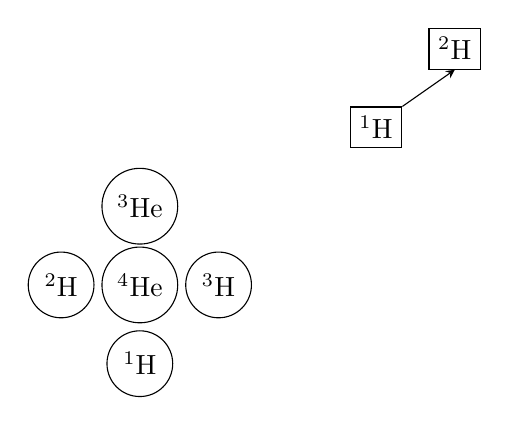
\begin{tikzpicture}
	\path ( 0,2) node [shape=circle,draw] {$\mathrm{{}^{3}He}$}
	( 0,1) node [shape=circle,draw] {$\mathrm{{}^{4}He}$}
	( 0,0) node [shape=circle,draw] {$\mathrm{{}^{1}H}$}
	( 1,1) node [shape=circle,draw, swap] {$\mathrm{{}^{3}H}$}
	
	(-1,1) node [shape=circle,draw] {$\mathrm{{}^{2}H}$};
	
%	\draw (3.7, 3) arc [
%		start angle =60,
%		end angle = 300, 
%		radius = 20pt,
%		color = blue
%	];
	
	%draw [color=blue] (3, 3) circle [radius = 20pt];
	%\draw (4, 3) circle [radius = 20pt];
	
	%(4, 4) node {$\mathrm{{}^{2}H}$};
	
	\node[draw, rectangle] (2H) at (4, 4) {$\mathrm{{}^{2}H}$};
	\node[draw, rectangle]  (1H) at (3, 3) {$\mathrm{{}^{1}H}$};
	
	\draw[-stealth] (1H.north east) -- (2H.south);
	
	%\draw (4, 4) node (A) {$A$} -- (5,5) node (B) {$B$};
	
\end{tikzpicture}
\end{center}

	\caption[Nuclear reactions chart]{Nuclear reactions chart (under elaboration)}
	\label{fig.nuclerReactionChains}
\end{figure}

\subsection{Classification of reactions} \label{sub:classificationReactions}

There are a vast variety of reactions in the astrophysical context. Most of them are classified depending on the interactions involved, the kind of reactant and product nuclei or their relevance in a particular astrophysical environment. This section pretends to give a broad classification of the reactions of interest in this document.\\ 

Most of the relevant reactions to be studied are of the form: 

\begin{equation} \label{eq:nuclearReaction_general}
	0 + 1 \rightarrow 2 + 3,
\end{equation}

where the pairs $0$ and $1$, $2$ and $3$ represent the reactant and product pairs respectively. However, there are processes which involve more than two reactants and products. \\

Also, there are some processes involving photons $\gamma$. Reactions with this characteristics are called radiative and their general form is the following:

\begin{equation} \label{eq:nuclearReaction_gammaCapture}
		0 + 1 \rightarrow 2 + \gamma.
\end{equation}

Additionally, electrons and neutrinos can be also incorporated to the reactions, specially in processes mediated by the weak force.  \\

Depending on the nature of the interaction involved in a particular process, a reaction can occur in a higher, medium and lower rates for nuclear, electromagnetic and weak force mediated processes. \\

In the upcoming subsections, a general description of reactions of considerable interest for the document is given. Reaction kinds such scattering, capture, exchange and fusion are given. 

\subsubsection{Scattering reactions} \label{ssub:scatteringReactions}

The first kind of reaction to be studied is scattering. In this case there is no change in the kind of nuclei. There is a subdivision depending if energy is conserved between the reactant nuclei. If it is such case, the scattering is elastic. Otherwise, it is inelastic. \\

The process of elastic scattering can be described, in classical terms, by nuclei get deflected after interacting as it is given in the following equation

\begin{equation}  \label{eq:nuclearReaction_scattering_elastic}
	A + a \rightarrow A + a.
\end{equation}

Notice that the process has the form of $A(a, a)A$ where $A$ and $a$ are the interacting nuclei. \\

On the other hand, the inelastic scattering proceeds similarly to the elastic case with the crucial difference that the final states of the nuclei might not have arrived with the same energy as the initial counterpart. For example, a nucleus can be excited after the interaction and, then, it is possible to claim that energy was not conserved. An example of this case can be represented by:

\begin{equation}  \label{eq:nuclearReaction_scattering_inelastic}
	A + a \rightarrow A^{*} + a,
\end{equation}

where the $*$ symbol is an indicator that the initial $A$ nucleus ended up in an excited state, which is annotated as $A^{*}$. In these cases, usually the $a$ nucleus is considerably lighter than $A$.\\ 

Alternatively, there are more inelastic outcomes, or channels, that can be present in the scattering picture. Particularly, they can be expressed as: 

\begin{equation}  \label{eq:nuclearReaction_scattering_inelastic2}
	\begin{split}
	A + a 	&\rightarrow A + a^{*} \\
				&\rightarrow A^{*} + a^{*}.
\end{split}
\end{equation}

where $a^{*}$ is the excited version of the $a$ nucleus. \\

Each of these two cases are relevant for astrophysical contexts. The elastic scattering is a common process critical to be accounted in the calculation of abundances. Additionally, excited states can be associated with resonances which are characteristic features of the behavior of a particular reaction and they increase the probability of interacting. \\

\subsubsection{Capture reactions} \label{ssub:captureReactions}

Also, radiative capture processes are considered at astrophysical energies. Various models could be used for determining potentials. There are clusters and potential models.

\begin{equation}  \label{eq:nuclearReaction_capture}
	X + c \rightarrow  \gamma + X'.
\end{equation}

When $c$ is a proton, the reaction is called radiative proton capture \cite{brune_davids_2015}. In addition, under certain circumstances, $c$ can also be an alpha particle. 

This kind of reactions are usually slower than exchange reactions. Therefore, radiative capture reactions constrain the entire rate of the chain they belong to. For example, in the CNO cycle, the reaction rate of the cycle is given by the rate of the $\CRadiativeCapture$ reaction. \\

Radiative capture appears in various element production contexts like pp chain, CNO cycle and also in explosive environments like X-ray burst and supernovae. There is a particular importance of the reaction $\BeRadiativeCapture$ since its product is a part of the triple alpha chain, which eventually results in the production of $\mathrm{{}^{12}C}$. In turn, the last nucleus is of crucial importance to the production of heavier elements. 

\subsubsection{Exchange reactions}  \label{ssub:exchangeReactions}

Another common reaction happens when there are two reactants and two products. This process is expressed by:

\begin{equation}  \label{eq:nuclearReaction_exchange}
	X +  x_1 \rightarrow x_2 + X'.
\end{equation}

A case of special interest occurs when $X$ and $X'$ are considerable heavier than $x_1$ and $x_2$ nuclei. Then, this process can be regarded as if the $x_1$ and $x_2$ nuclei where exchanged, while the heavier nucleus $X$ transforms to $X'$. \\

This reaction proceeds depending which is the heaviest nuclei. In particular, there are two main mechanisms: stripping and pickup \cite{xu_takahashi_goriely_arnould_ohta_utsunomiya_2013}.\\ 

Stripping follows when $X'$ is heavier than $X$, and therefore $x_1$ is heavier than $x_2$. The form of this process is given by:

\begin{equation}  \label{eq:nuclearReaction_exchange_stripping}
	\begin{split}
		x_1		&\rightarrow x  +  x_2 \\
		X + x 	&\rightarrow X'.
	\end{split}
\end{equation}

On the other hand, pickup  occurs when $X$ is heavier than $X'$, and thus $x_2$ is heavier than $x_1$. This channel proceeds like:
 
 \begin{equation}  \label{eq:nuclearReaction_exchange_pickup}
 	\begin{split}
 		X 			&\rightarrow x + X' \\
 		x_1 + x  &\rightarrow x_2.
 	\end{split}
 \end{equation}

It is essential to be noticed that both reactions follow a two step process. The first step consists of a decay reaction with the particularity that it produces the nucleus $x$, which serves as a reactant in the following merging reaction. Ultimately, since $x$ appears in both sides on the two possible processes,  it is not distinguished neither as a product nor as a reactant in the simplified form of the exchange reaction of equation \ref{eq:nuclearReaction_exchange}. \\

A thorough description of this reaction is given by the distorted wave Born approximation DWBA. This broadly consists of using two potentials, one for each pair of reactants and products, and the other for the picking or stripping interaction. More detains are given in section \ref{ssub:potential_calculations_exchange}. \\

A development on the $\mathrm{(p,n)}$ reaction kind is given by (Distorted wave Born approximation DWBA model) \cite{whitehead_poxon-pearson_nunes_potel_2022} and for the $\mathrm{(n,p)}$ in (Weisskpf-Ewing) deformation without spin description \cite{sharma_gandhi_kumar_2022}. \\

$\ddexchange$ is an example of an exchange reaction relevant for BBN and pp-chain nucleosynthesis. 


\subsubsection{Fusion reactions} \label{ssub:fusionReactions}

Although most of reactions in the nuclear astrophysical context can be regarded as fusions, the term is usually reserved when referring to reactions of the form:

\begin{equation}  \label{eq:nuclearReaction_fusion}
	X + Y \rightarrow a + X',
\end{equation}

where $X$, $Y$ and $X'$ are heavier nuclei than the product $a$. Reactions with $X = Y$ are pivotal in stellar nucleosynthesis as it will be seen in section \ref{sec:StellarFusion}.

\subsection{Kinematics} \label{sub:kinematics}

Definition of the $Q$ value. This determines if the reaction is exothermic or endothermic and thus it estimates the favorability of the process. This quantity is defined as: 

\begin{equation}\label{eq:nuclearReaction_Qvalue}
	Q = (\sum m_{\mathrm{react}} - \sum m_{\mathrm{prod}})c^2,
\end{equation}

where $\sum m_{\mathrm{react}}$ and  $\sum m_{\mathrm{prod}}$ correspond to the sum of the reactant and product nuclei respectively. If $Q > 0$, it means that energy was released and the reaction is exothermic. Reciprocally, in the case $Q < 0$ energy is absorbed and therefore the reaction is endothermic.  \\

Center of mass frame is preferred since there multiple nuclei are interacting as a common system. Then, kinematical variables shall be converted to the center of mass frame. Such transformations can imply coordinate changes. For instance, the center of mass of a two body system $\vec R$ is given by: 

\begin{equation}\label{eq:nuclearReaction_centerOfMass}
	\vec R = \frac{m_a \vec r_a + m_b \vec r_b}{m_a + m_b},
\end{equation}

where $m_a$ and $m_b$ are the masses and $\vec r_a $ and $\vec r_b$ are the positions of the reacting $a$ and $b$ nuclei respectively. \\

Another consequence of this introduction is a change on the shape of the Schrödinger equation. For a two body with $a$ and $b$ initial nuclei, without considering centrifugal effects, the Hamiltonian is given by: 

\begin{equation}\label{eq:nuclearReaction_hamiltonian_twoBody}
	H = - \frac{\hbar^2}{2m_a} \nabla^2_a  - \frac{\hbar^2}{2m_b} \nabla^2_b + V_{ab}(r),
\end{equation}

with $\nabla^2_a$ and   $\nabla^2_b$ being the Laplacian operators corresponding to the  $\vec r_a $ and $\vec r_b$  coordinates respectively. Additionally, the central potential $ V_{ab}(r)$ is given in terms of a relative distance $r$ which is defined as $r = |\vec r_a - \vec r_b|$. \\

When the center of mass coordinates are used, it is possible to transformed the two body picture of equation \ref{eq:nuclearReaction_hamiltonian_twoBody} as: 

\begin{equation}\label{eq:nuclearReaction_hamiltonian_centerMass}
	H = - \frac{\hbar^2}{2\mu} \nabla^2  + V_{ab}(r),
\end{equation}

where the Laplacian $ \nabla^2$ is defined with center of mass coordinates and the reduced mass $\mu$ is defined as: 

\begin{equation}\label{eq:nuclearReaction_reducedMass}
	\mu = \frac{m_a m_b}{m_a + m_b}.
\end{equation}

\subsection{Cross sections} \label{sub:crossSections}

Cross section of a process is defined within the center of mass frame. In particular, a single particle quantum mechanical picture, with variables appropiartely defined in the frame of the center of mass, can represent a two-body interaction, which is usually the case for nuclear reaction. \\

A connection between the cross sections and quantum mechanical variables is given by: 

\begin{equation}\label{eq:nuclearReaction_crossSection_quantumMechanics}
	\sigma = \frac{j_c r^2 }{j_b},
\end{equation}

where $j_b$ and $j_c$ are the magnitudes of the incident and outgoing current density probabilities respectively. Notice that the factor of $r^2$ gives $\sigma$ its characteristic area units. \\

There is not a unique way of determining the partial and total cross sections since its determination heavily depends  on the reaction type. Chapter \ref{ch:sfactorCalculations} is dedicated for considering multiple cross section calculations. Still, as anticipated from scattering theory, cross sections have relations with the $S$-matrix. \\

The center of mass is defined closely with the quantum mechanical definition. Particularly, the definition must consider the two body problem, which is usually the case for nuclear reactions. \\

If a channel of the form $a + A \rightarrow b + B$ is considered, and its cross section $\sigma_{aA \rightarrow bB}$ is known, it is possible to information for the reciprocal reaction, which is defined as  $ b + B \rightarrow a + A$. Particularly, the cross section of the reversed reaction $\sigma_{bB \rightarrow aA}$  is given by  \cite{iliadis_2015}:

\begin{equation}\label{eq:nuclearReaction_reciprocal}
	  \sigma_{bB \rightarrow aA} = \frac{k^2_{aA}}{k^2_{bB}} \frac{(2j_a + 1)(2j_A + 1) }{ (2j_b + 1)(2j_B + 1) } \frac{1 + \delta_{bb}}{1 + \delta_{aA}} \sigma_{aA \rightarrow bB} ,  
\end{equation}

where the pair $k_{aA}$, $k_{bB}$ corresponds to the wave vectors associated with the reactants ans products respectively. The pairs $j_a$ with $j_A$ and $j_b$ with $j_B$ are associated with the total angular momentum number for their corresponding reactant and product nuclei respectively. Additionally, the terms $\delta_{aA}$ and  $\delta_{bB}$ are equal to one only if the indexed nuclei are the same, otherwise their value is zero. The introduction of this term accounts for corrections to the cross section when nuclei are indistinguishable. 

\subsection{Reaction rates} \label{sub:reactionRates}

The ratio that determines the number of nuclei per unit per unit volume time to be consumed is given by: 

\begin{equation}  \label{eq:reactionRate_generic}
	r_{ab} = N_aN_b \langle \sigma (v)  v \rangle,
\end{equation}

where $\sigma(v)$ is the cross section of a reaction, which depends on the relative speed $v$ of the $a$ and $b$ reactant nuclei. $N_a$ and $N_b$ are the number of $a$ and $b$ nuclei per unit volume respectively. Additionally, the  product $\sigma (v) v$ can be interpreted physically as a sort of flux of the reaction. \\

It is critical to observe that, rather than being a definite variable, the relative speed of the colliding nuclei has a spectrum of possible values. Particularly, at thermal equilibrium and non relativistic speeds, which is strongly predominant in most nuclear astrophysical scenarios, the Maxwell-Boltzmann distribution is preferred. The probability of finding a pair of nuclei with relative velocity  between $v$ and $v + dv$ is given by:

\begin{equation} \label{eq:reactionRate_maxwellBoltzmann}
	P(v)dv = 4\pi \left( \frac{\mu}{2\pi kT}\right)^{3/2} v^2 \exp{\left({\frac{\mu v^2}{2kT}}\right)}dv.
\end{equation}


where $\mu$ is the reduced mass of the reactant nuclei,  $k$ is the Boltzmann constant and $T$ is the reservoir temperature. Then, the average reaction flux $\langle \sigma v \rangle $, expressed in terms of the center of mass energy $E$, is given by \cite{ueda_sargeant_pato_hussein_2004}:

\begin{equation}  \label{eq:reactionRate_definition}
	\langle \sigma(v) v \rangle = \left(\frac{8}{\pi \mu (kT)^3 }\right)^{1/2}  \int_0^{\infty} { E \sigma(E) \exp\left({-\frac{E}{kT}}\right)  dE},
\end{equation}


A notable exception of this rule happens when a photon is one of the reactants. In that case, $v = c$ as special relativity imposes. On the other hand, since the photon is a relativistic boson, it is required the use of the Bose-Einstein statistics, which is defined as:  

\begin{equation} \label{eq:reactionRate_boseEinstein}
	P(E)dE = \frac{8\pi}{(hc)^3} \frac{E^2}{\exp{\left(\frac{E}{kT}\right)} - 1}.
\end{equation}

In this case $E$ represents the photon energy and $\sigma(E)$ is interpreted as the photon absorption cross section.


On specifying the rates, it is needed to be considered.

Reaction rates are considered from calculation of transmitted, incident and interacting 
- Reaction rate depends on the density of particles, the velocity and the cross section
-	It is averaged by a convenient distribution. (Maxwell-Boltzman for fermions, Bose Einstein (Planck) for photons)
-	With the rates, abundance evolution is determined 

 For particles of matter, the statistics at the star fusing scale is Maxwell - Boltzmann and for photons the Bose - Einstein statistics. \\ 


There are extensions to the Maxwell-Boltzmann treatment. For example, more general distribution functions are used such as the Tsallis statistics \cite{haubold_kumar_2008}.  \\

There are special considerations and approximations for the case of resonances. If they are sufficiently broad, the Breit-Wigner like dependence can be dropped out of the reaction rate integral. \\

 Reaction rates are fundamental in calculating the element ratios, which are determined by differential equation solving. Computation of the abundance of elements can be a complex task considering the fact that a nuclei can be produced or annihilated by multiple processes. A master equation for the time calculation of the abundance $N(t)$ of a particular nucleus is given by:
 
 \begin{equation}\label{eq:reactionRate_abundances}
 	\frac{dN}{dt} = \lambda_1 N_1(t) + \lambda_2 N_2(t)  + ... -  \lambda_1' N_1'(t) + \lambda_2' N_2'(t),
 \end{equation}

where $N_1(t), N_2(t), ...$ and $N_1'(t), N_2'(t), ...$ are the abundances of the elements which produce and consume the nucleus respectively. Similarly,  $\lambda_1, \lambda_2, ...$ and  $\lambda_1', \lambda_2', ...$ are quantities associated with the decay rates favorable and unfavorable to the production of $N$ respectively. It is central to be noticed that the abundance of an element usually depends of the abundances of other nuclei. Consequently, in order to actually equations like \ref{eq:reactionRate_abundances}, it is necessary to solve all the abundances simultaneously by solving a system of differential equations with all the relevant nuclei to be considered. Since abundance equations are first order, it is necessary, in addition to estimate the reaction rates, to guess an initial distribution of the elements in the Universe. The details on this selection is still a topic of active research. \\

However, equation \ref{eq:reactionRate_abundances} does not take into account the reaction rates of cross section. In order to do so, it is necessary to include the abundances of the process involved in a reaction. For example, the contribution to equation \ref{eq:reactionRate_abundances} of the channel $a + A \rightarrow b + B$ is going to be proportional to: 

\begin{equation}
		\left(\frac{dN}{dt}\right)_{aA \rightarrow bB} \sim r_{aA \rightarrow bB},
\end{equation}

where $N_a(t)$ and $N_b(t)$ are the abundances of the reactant nuclei and $ \sim r_{aA \rightarrow bB}$ is the reaction rate of the channel. This contribution can be positive or negative depending if the $N$ nuclei are produced or consumed by the reaction respectively. Therefore, a generalization of equation \ref{eq:reactionRate_abundances}, with the contributions of the cross sections, is given by: 

\begin{equation}\label{eq:reactionRate_abundances_general}
	\frac{dN}{dt} =  \sum_{k} {\lambda_k N_k}  - \sum_{l} {\lambda_l N_l} +  \sum_{m, n} {r_{mn}} - \sum_{o} {r_{o}},
\end{equation}

where the indices $k$ and $l$ tag the decays producing and consuming respectively. Additionally, the $m, n$ pair of indices corresponds to the nuclei which react to produce $N$ at a rate $r_{mn}$. Thus, the sign associated to this contribution is positive. Finally, the index $o$ accounts for the nucleus that consumes $N$ in a reaction with rate $r_0$. Therefore, its contribution is negative. \\

There are broad classification of reactions. 

\section{The Astrophysical S-factor} \label{sec:sFactor}

Cross section does not count for the low-energy behavior. Then, additional factors can be obtained. For example, S-factor.
\subsection{Definition} \label{sub:sfactorMotivationDefinition}

There are S factors associated with the energy and they are the path to determine the nature of the potential, which is not necessarily a Yukawa potential.

\begin{equation} \label{eq:sfactor_definition}
	S(E) = E \exp({2\pi\eta}) \sigma({E}).
\end{equation} % ISBN 978-0-521-85635-5.

It is directly proportional to the microscopic cross section of the process $\sigma(E)$ and it represents the rate of a certain nuclear reaction.  \\

In particular, the astrophysical S-factor scales the cross section with an exponential factor $\exp({2\pi\eta}$ which compensates the Coulomb repulsion damping. In particular, the $\eta$ factor is defined as 

\begin{equation} \label{eq:sfactor_sommerfeld}
	\eta = \frac{Z_1Z_2e^2}{4\pi\epsilon_0\hbar v}
\end{equation}

where $v$ corresponds to the relative speed between the reactants. At the same time, this speed can be expressed in terms of $E$, which is interpreted as the center of mass energy, as given by: \\

\begin{equation}\label{eq:sfactor_speed}
	v = \sqrt{\frac{2E}{\mu}},
\end{equation} 

where $\mu$ corresponds to the reduced mass of the reactant nuclei. \\

On the other hand, the linear factor $E$ is included in the S-factor definition in order to compensate the effect that the quantum mechanical $1/k^2 \propto 1/E$ factor adds to the cross section. \\

There is a strong relation of the astrophysical $S$ factor with the center of mass energy. 

Usually this relation depends on the square of the energy of the center of mass $E_{\mathrm{cm}}$. \\

There are topics that are relevant in the frontiers of nuclear astrophysics  \cite{bertulani_kajino_2016} (classification with all the nuclear astrophysics environments). 

\subsection{General applications} \label{sub:sfactorApplications}

Empirical fitting of cross section and reaction rates. \\

Cross section extrapolation to low energies. \\

Reaction rates and element abundance estimations. 

\chapter{Reactions of astrophysical interest}  \label{ch:reactionsInterest}

Nuclear reactions are part of the core of nuclear astrophysics. They are accountable for the production mechanism of elements in several astrophysical environments where thermonuclear reactions can occur. In particular, there are specially relevant reactions for the explanation of the abundance of elements. For example, some of these reactions are part of critical fusion chains of stars, have challenging extrapolation techniques to low energies, or  exhibit exotic underling physical phenomena.   \\

In this section, a relevant selection of reactions types of will be reviewed.  Several reaction kinds and models are given and the classification of potential, R-matrix and microscopical models are illustrated in \cite{descouvemont_2020}.



\section{Big Bang nucleosynthesis} \label{sec:BBN}

Primordial reactions that where expected to happen just after the Big Bang occurred. For example, a reaction which is vital for the formation of hydrogen, the first element, is given by: 

\begin{equation} \label{eq:reaction_BBN_np}
	n \leftrightarrow p + e^{-} + \bar v_{e}. 
\end{equation}

Notice that the previous reaction, rather than being a one direction process, is a two sides reaction. In particular, the equilibrium constant was expected to shift towards the products, and therefore it involved the production of protons, as the Universe cooled down. \\

Later, in a period ranging from seconds to a couple of minutes after the beginning of the Universe, radiation damped to the point where atomic configurations were more likely than electromagnetic disintegrations. Then, the first hydrogen atoms where formed and, as the Universe temperature decreased, the first fusion reactions appeared.  \\

Seconds to minutes after the Big Bang. 

Neutron and proton stability difference. Neutrons are unstable.  Shift towards protons permits fusion. 

Two conditions: the feasibility to fuse and the disintegration stability.

Balance between photons and baryons. If photons density exceeds too much the number of baryons, disintegration dominates. 

Deuterium is the first nuclear fusion product, since it  consists of a proton and a neutron. began to fuse when photons had  energy lower than the binding energy of deuterium nuclei. 

Relaxation times and deuterium fusion possibility. Eventually, Universe cooling inhibited additional fusion. An example of a radiative capture reaction involving deuterium is given by:

\begin{equation} \label{eq:reaction_2Hpradiative}
	\mathrm{{}^{2}H + p \rightarrow \gamma + {}^{3}H}.
\end{equation}

This is a process which produces tritium $\mathrm{{}^{3}H}$. This product serves as the starting point of a fusion chain going up to $\mathrm{{}^{7}Be}$. However, new evidence has shown that this process could had extended up to middle heavy nuclei like carbon, nitrogen and oxygen isotopes.

BBN description \cite{coc_vangioni_2010}
Review \cite{patrignani_et_particle-data-group_2016}.

Elements very high temperatures \cite{wagoner_fowler_hoyle_1967}

Even CNO elements can be produced via BBN nucleosynthesis under specific conditions \cite{su-qing_kai-su_yong-shou_neng-chuan_zhi-hong_2010}.

Unlike other abundances of lighter elements, lithium abundance is not well explained by Standard Big Bang theory \cite{bertulani_2019}. 


\section{Stellar fusion}  \label{sec:StellarFusion}

Much after the Big Bang, stars are formed through a process of compaction of gases, which is made mostly of hydrogen. The high temperature and density environment of the core of stars allows the activation of various fusion reactions.  \\

Stellar stability is the result of the hydrostatic equilibrium established by the compensation compressing gravitational effect with the repulsive radiation pressure exerted fueled by the fusion reaction produced at the core of the star. The mechanisms of heat exchange in stars are radiation and convection. \\

The diversity of elements fusing at the core of a star heavily depends on the kind of star and the stage in the stellar evolution.  Initially, when temperature and density have reached critical values, the fusion process begins. In particular, hydrogen is the first element source of fusion reactions. \\

The classical treatment of fusion in stars is given by the classical \cite{burbidge_burbidge_fowler_hoyle_1957}. \\

Summary text with aspects of stellar evolution, degenerate stars and more \cite{kundt_2005}. \\

Hertzsprung-Russel diagram permits a classification of a star with respect to specific categories which are related to different evolution stages in the lifetime of a star \cite{arsentieva_shevchenko_2021}. It classifies stars in clusters depending on their collective luminosity and magnitude characteristics. \\

Brown dwarfs are the first of such classifications. This objects with stellar magnitude which where unable to produce a sustainable chain of fusion of hydrogen. As a result, their luminosity is generally low. Their masses are roughly bounded by $M < 0.07M_{\odot}$. \\

Red dwarfs are the smallest objects which are able to sustain a chain of nuclear fusion reaction. Their color is red and their mass $ 0.07M_{\odot} < M < 0.5 M_{\odot} $ and low luminescence. Most of the stars on the Universe are in this group. However, at these mass values they are unable to burn helium \cite{kundt_2005}. \\

Main sequence branch, which is the current classification of the Sun, includes stars with middle mass with $ 0.5M_{\odot} < M < 2M_{\odot}$ approximately. Their color leans usually to yellow. They grow during their live until they reach a red giant stage. \\

Asymptotic red giant is a superstar with the mass of $M > 2M_{\odot}$. They fuse $\mathrm{{}^{4}He}$ and even isotopes of carbon. Some stars of this kind releases their material without explosion, like the case of the sun, while others are massive enough to collapse as a supernova given certain conditions which are going to be generally sketched later. In fact, it is critical to be annotated that mass is not the only criteria when determining the outcome of a star since variables like nuclear composition, density, angular momentum are eventually relevant.  \\

The supergiant and hypergiant are stars with high mass $M > 3M_{\odot}$ and gigantic size with radii $R > 1000R_{\odot}$. These stars are usually involved in highly explosive environments. One common kind are supernovae of kind AII, which is a mechanism of core collapse for stars that have reached iron as their ultimate product. On the other hand, a less common, although more explosive, is a supernovae of kind IA, which usually involve a binary system consistent of a red giant and a white dwarf. \\

White dwarfs are the remnants of the life of active stellar fusion. Their radius is close to the radius of the earth. Their stability is explained by repulsion degeneracy of their exterior layer of electrons. It is quite remarkable that this star is able to maintain hydrostatic equilibrium with mostly quantum mechanical originated degeneracy pressure.  Actually, these kind of stars are critical for certain kinds of supernovae. \\ 

Neutron stars are compact objects which, like the white dwarfs, does not perform large scale fusion sustainable reactions. Instead, their stability is explained by the repulsion generated by the fermionic degeneracy of its constituent neutrons. This explains the extremely compact nature of this objects since a mass times larger than the sun is occupied within an object with radius of a couple of tenths of kilometers long. \\ 

Therefore, they are one of the most dense objects in the universe.  It has been speculated that  at the interior of these objects, a new state of matter, which is usually called the quark gluon plasma, is possible given the extreme conditions of degeneracy at these environments.\\ 

The next step in compactness are black holes. This objects have self collapsed gravitationally to the point that even light cannot escape the gravitational binding at regions inside the event horizon. A first approach towards determining the mass limit of a star to become a black hole is known as the Chandasekar mass, which corresponds to 2.4 solar masses. However, a complete calculation should take into account particularities on the initial configuration of the star like its metallicity and element composition.  \\

Introduce the needed conditions for the creation of stars in the primordial nebula.\\

Describe how the hydrogen is burnt in the star's core and the associated products.  \\


Explain the required conditions that permits nuclear fusion in the star's nucleus.

\subsection{Light heavy nuclei reactions} \label{sub:lightReactions}

Fusion reaction at stars start with hydrogen, which is originated from the Big Bang. Then, at the hot center of stars, a long process to produce $\mathrm{{}^{4}He}$. The nuclear chain which is central in this transition is the pp chain. \\

Next, if stars are high temperature enough, further heavy elements are produced from helium burning. This process is known as the triple alpha chain in where $\mathrm{{}^{12}C}$ and $\mathrm{{}^{16}O}$  nuclei are produced. They perform a series of cycles, which are referred as CNO. Also, for explosive and highly energetic environments, the alternative cycles HCNO are also present at stellar environments.  \\

At the end of the life of big stars, reactions of the form $\Cfusion$ and $\Ofusion$ take place. Heavier nuclei are produced. Then neon and silicon burning occurs. With silicon burning, neon is produced. 

\subsubsection{pp chain}

Much of the initial fusion at the core of a great extent of lifetimes of main branch stars like the sun consist on hydrogen fusion reactions. The interactions of pp-chain processes are mostly electromagnetic and strong force with additional weak force mediated reactions. In addition, reaction rates of nuclear fusion processes depend on the interaction cross section and the abundance of the reactant nuclei. \\

Particularly, the critical pp reaction is mediated by the weak force. As a consequence of this fact, reaction times are long and therefore stars can sustain their stability driven by hydrostatic equilibrium for billions of years. 

pp chain review \cite{fowler_1958}. \\

The main reaction in which this process occurs is: 

\begin{equation} \label{eq:reaction_ppMain}
	p + p \rightarrow d + e^{+} + \nu_e.
\end{equation}

Then, when deuterium is available, there is the possibility of production of tritium $t$, which is a name for the  $\mathrm{{}^{4}He}$ nucleus,  in a reaction of the form:

\begin{equation} \label{eq:reaction_2Hdn3He}
	d + d  \rightarrow n + {}^{3} \mathrm{He}.
\end{equation}

Alternatively, another tritium producing  fusion reaction involving deuterium fusion is given by:

\begin{equation}  \label{eq:reaction_2Hdpt}
	d + d \rightarrow p + t.
\end{equation}

Tritium production opens different branches for the pp-chain. For example, the main branch proceeds like: 

\begin{equation} \label{eq:reaction_3Hep3He}
	{}^{3}\mathrm{He} +  {}^{3}\mathrm{He}  \rightarrow {}^{4}\mathrm{He} + 2p.
\end{equation}

This process in known as the pp1 chain. On the other hand, a more unlike second branch named pp-II follows as :

\begin{equation} \label{eq:reaction_3HepChain}
	{}^{3}\mathrm{He} + p \rightarrow {}^{4}\mathrm{Li} + \gamma \rightarrow {}^{4}\mathrm{He} + e^{+} +  \nu_e + \gamma.
\end{equation}

This process is unlikely because of the instability of  ${}^{4}\mathrm{Li}$, which decays to ${}^{3}\mathrm{He}$.

Lastly, an additional third branch is yet possible called pp-III given by: 

\begin{equation} \label{eq:reaction_3HepChain_III}
	{}^{3}\mathrm{He} + n \rightarrow {}^{4}\mathrm{He} +  \gamma.
\end{equation}

As it is seen in the previous reactions, this chain ends with the production of $\mathrm{{}^{4}He}$. The chain stops here because this is the most stable nucleus of the light nuclei class. Additionally, this resulting nucleus is a relevant source of the production of heavier nuclei, in particular of the triple alpha process reactions.

Additionally, screening effect present in light weight nuclear reactions \cite{raiola_migliardi_gyurky_aliotta_formicola_bonetti_broggini_campajola_corvisiero_costantini_et_2002} and a review of screening effect \cite{assenbaum_langanke_rolfs_1987}.

\subsubsection{Triple alpha process}

When $\mathrm{{}^{4}He}$ abundance, as well as temperature and density conditions are sufficient enough to fuse helium, the triple alpha process takes place. This conditions are not necessarily reached in all stars. In fact, the sun reaches this process at the last period of its lifetime.  

Triple - alpha process review \cite{coc_2012}.

The process is called triple alpha because it consist of three reactions involving $\alpha$ particles, which are equivalent to  $\mathrm{{}^{4}He}$ nuclei. 

\begin{equation}\label{eq:reaction_tripleAlpha_1}
	\mathrm{{}^{4}He + {}^{4}He \rightarrow  \gamma  + {}^{8}B }
\end{equation}

The next instance:

\begin{equation}\label{eq:reaction_tripleAlpha_2}
	\mathrm{{}^{8}B+ {}^{4}He \rightarrow  \gamma + {}^{12}C}. 
\end{equation}

Finally, 

\begin{equation}\label{eq:reaction_tripleAlpha_3}
	\mathrm{{}^{12}C + {}^{4}He \rightarrow \gamma + {}^{16}O}.
\end{equation}

The resulting nuclei of this process is $\mathrm{{}^{16}O}$, which is a very stable nuclei since it is double magic. This reaction completes with the production of another stable nuclei like $\mathrm{{}^{12}C}$. These two nuclei will have a substantial role in the production of heavier elements at the last stages of giant stars.

\subsection{CNO cycle}  \label{sub:CNOCycle}

When the star has capacity of completing the triple alpha process, their subproducts are available for additional nuclear reactions. In particular, with the presence of $\mathrm{{}^{12}C}$ nuclei, a series of capture reactions take place. These reactions will form cycles.

CNO cycle reactions \cite{wiescher_gorres_schatz_1999}.

 The first cycle reactants include carbon, nitrogen and oxygen isotopes. The reaction proceeds as:  

\begin{equation} \label{eq:reaction_CNO_C}
	\mathrm{{}_{6}^{12}C  \rightarrow {}^{13}_{7}N  \rightarrow {}^{13}_{6}C  \rightarrow {}^{14}_{7}N  \rightarrow {}^{15}_{8}O  \rightarrow {}^{15}_{7}N \rightarrow {}^{12}_{6}C}.
\end{equation}



The last cycle fuels another nuclear capture cycle. In this case, the starting point are $\mathrm{{}^{15}N}$ nuclei and the cycle also involve oxygen and fluorine isotopes. In particular, the cycle is given explicitly by the reaction chain: 

\begin{equation} \label{eq:reaction_CNO_N}
	\mathrm{{}_{7}^{15}N  \rightarrow {}^{16}_{8}O  \rightarrow {}^{17}_{9}F  \rightarrow {}^{17}_{8}O  \rightarrow {}^{14}_{7}N  \rightarrow {}^{15}_{8}O \rightarrow {}^{15}_{7}N  }.
\end{equation}

There is even a third CNO cycle, which is far more uncommon and there fore is considerably less dominant than the second and first CNO cycle. In this case, the process is given by: 

\begin{equation} \label{eq:reaction_CNO_O}
	\mathrm{{}_{8}^{17}O  \rightarrow {}^{18}_{9}F  \rightarrow {}^{18}_{8}O  \rightarrow {}^{15}_{7}N  \rightarrow {}^{16}_{8}O  \rightarrow {}^{17}_{9}F \rightarrow {}^{17}_{8}O  }.
\end{equation}

All of the previous cycles are coupled in the sense that the production of one element in one cycle may affect another cycle. In particular, CNOI fuels CNOII which at the same time feeds the CNOIII cycle. Particularly, Also notice that the three cycles begin with nuclei with consecutive atomic number. More concretely, carbon, nitrogen and oxygen nuclei begin the CNOI, CNOII and CNOIII cycles respectively.\\

There is also a CNOIV cycle, which is a version of the CNOIII with heavier nuclei. However, it is much less dominant than the CNOI cycle and relevant only in stellar fusion on heavy stars. The cycle is given by:

\begin{equation} \label{eq:reaction_CNO_O_4}
	\mathrm{{}_{8}^{18}O  \rightarrow {}^{19}_{9}F  \rightarrow {}^{16}_{8}O  \rightarrow {}^{17}_{9}F  \rightarrow {}^{17}_{8}O  \rightarrow {}^{18}_{9}F \rightarrow {}^{15}_{8}O }.
\end{equation}


The last three processes are summarized in the illustration of Figure \ref{fig:CNOcyles}.

\begin{figure}[H]
	\tdplotsetmaincoords{80}{155}
\usetikzlibrary{3d}

\begin{center}
	\begin{tikzpicture}[scale = 5, tdplot_main_coords]		
	
		\draw[-{Stealth[scale=2]}, blue] (0, 1) -- (1, 0);
		
		\draw[-{Stealth[scale=2]}] (1, 0) -- (0.5, -1);
		
		
		\draw[-{Stealth[scale=2]}]  (0.5, -1) -- (-0.5, -1);
		
		\draw[-{Stealth[scale=2]}] (-0.5, -1) -- (-1, 0);
		
		\draw[-{Stealth[scale=2]}] (-1, 0) -- (0, 1);
	
		
	\end{tikzpicture}
\end{center}

	\caption[CNO I, II and III cycles representations]{CNO I, II and III cycles representations. Notice how the byproducts of the preceding cycles are sources of the next cycle. This figure is under elaboration.}
	\label{fig:CNOcyles}
\end{figure}

Notice that the cycle balance is established by the existence of proton capture and beta decay, which increases and decreases the atomic mass respectively. Then, any change in the rates of the previous reactions would alter the possiblity of production of certain elements. In particular, at high enough temperatures, the rate of the proton capture process surpass that of the beta capture. Then, alternative products are produced and new processes form what is called hot CNO cycles. \\ 

At explosive environments, the CNO cycle is altered and it forms a new cyclic reaction chain called the HCNO cycle, or hot CNO cycle.  New reactions are present given the more energetic conditions of this cycle. There are HCNOI, HCNOII and HCNOIII cycles, which are closely related with the CNOI, CNOII and CNOIII cycles respectively. For instance, the HCNOI proceeds as: 

\begin{equation} \label{eq:reaction_HCNO_C}
	\mathrm{{}_{6}^{12}C  \rightarrow {}^{13}_{7}N  \rightarrow \textcolor{blue}{{}^{14}_{8}O}  \rightarrow {}^{14}_{7}N  \rightarrow {}^{15}_{8}O  \rightarrow {}^{15}_{7}N \rightarrow {}^{12}_{6}C}.
\end{equation}

The painted term corresponds to the differing term in the cycle. Next, the HCNOII cycle is given by: 

\begin{equation} \label{eq:reaction_HCNO_N}
	\mathrm{{}_{7}^{15}N  \rightarrow {}^{16}_{8}O  \rightarrow {}^{17}_{9}F  \rightarrow \textcolor{blue}{{}^{18}_{10}Ne  \rightarrow {}^{18}_{9}F}  \rightarrow {}^{15}_{8}O \rightarrow {}^{15}_{7}N  }.
\end{equation}

The highlighted terms are not present permit the cycle to reach a Ne isotope and are not present in the CNOII cycle. Lastly, the HCNO-III cycle proceeds like: 

\begin{equation} \label{eq:reaction_HCNO_O}
	\mathrm{{}_{18}^{9}F  \rightarrow {}^{19}_{10}Ne  \rightarrow {}^{19}_{9}F  \rightarrow {}^{16}_{6}O  \rightarrow {}^{17}_{9}F  \rightarrow {}^{18}_{10}Ne \rightarrow {}^{18}_{9}F  }.
\end{equation}

In contrast to the previous hot cycles, HCNOIII does not begin with the same nucleus than its non hot analogous the CNOIII cycle. Instead, it begins at $\mathrm{{}_{18}^{9}F}$ and, like the CNOIV cycle, is also able to produce neon nuclei in the process. \\

Further cycles related to alpha reactions Ne cycle \cite{kaeppeler_wiescher_giesen_goerres_baraffe_eleid_raiteri_busso_gallino_limongi_et_1994}\\

There are more cycles of capture reaction. An example regarding the MgAl cycle is given in \cite{lotay_doherty_janssens_seweryniak_albers_almaraz-calderon_carpenter_champagne_chiara_hoffman_et_2022}.


\subsection{Medium heavy fusion reactions} \label{sub:mediumHeavyReactions}

At a certain moment, the core of big stars starts to contract. Then, various middle heavy elements start to be consumed by the star. These reactions concern nuclei with $A < 28$. Classical burning processes include carbon, neon, oxygen and silicon, as well as a whole new variety of processes are allowed given the appropriate conditions at the last period of the lifetime of the star. \\

Examples of this kind of reaction include the $\mathrm{{}^{12}C + {}^{12}C}$,   and the  $\mathrm{{}^{16}O + {}^{16}O}$ fusion reactions.   Most of these reactions result in different channels. \\


With respect to the carbon fusion reaction, which is the starting reaction,  the principal channel is given by: 

\begin{equation} \label{eq:reaction_C12fusion_alpha20Ne}
	\mathrm{{}^{12}C + {}^{12}C \rightarrow {}^{4}He + {}^{20}Ne}. 
\end{equation}

Additionally, carbon burning contributes to heavy nuclei production as being a source neutrons. In particular, the process that allows this production is given by:

\begin{equation} \label{eq:reaction_C12fusion_n23Mg}
	\mathrm{{}^{12}C + {}^{12}C \rightarrow n  + {}^{23}Mg}. 
\end{equation}

Later, oxygen burning starts are very high temperatures and pressures than the neon and carbon burning due to the high stability of oxygen nuclei. In fact, oxygen nucleus is double magic. The main channel of the oxygen fusion reaction occurs in the following manner:

\begin{equation} \label{eq:reaction_O12fusion_alpha28Si}
	\mathrm{{}^{16}O + {}^{16}O \rightarrow {}^{4}He + {}^{28}Si}. 
\end{equation}

The neutron producing channel related to oxygen burning, which is analogous to the reaction of Equation \ref{eq:reaction_C12fusion_n23Mg}, proceeds as: 

\begin{equation} \label{eq:reaction_O12fusion_n31S}
	\mathrm{{}^{16}O + {}^{16}O \rightarrow n + {}^{31}S}. 
\end{equation}

Actually, there are more carbon and oxygen fusion channels than the previously mentioned. Further channels are visualized in the reaction bifurcations which are presented in Figure \ref{fig:COchannels}. \\

Middle heavy fusion reactions have in common to have subbarrier energies in the range of the MeV. Additionally, at energies beyond the barrier, it is usual to encounter an almost non-resonant behavior on the cross sections. However, as the energy decreases, the effects of reactions are more noticeable. \\

Molecular effects are relevant in these nuclei. In particular, additional degrees of freedom like rotation or vibration allow the nuclei to deform and also to couple to different channels. Therefore, new transitions are possible and reaction probabilities are increased. \\

These nuclei are edgier to be described with clustering. For example, the $\Cfusion$ nuclei can be interpreted as a $3\alpha$ cluster. Similarly, the $\Ofusion$ has a structure of a $4\alpha$ embedding. Then, the interactions can be represented by nucleon-nulceon, or alternatively cluster-cluster. The first approach is privileged when calculations are performed with all the nuclei while the second approach assumes an effective interaction of the constituent alpha particles of the nuclei.  \\

\begin{figure}[H]
	\begin{center}
	\begin{tikzpicture}

		\node (center) at (0, 0) {$\mathrm{{}^{16}O + {}^{16}O}$};
		
		%\node (CH1) at (6, 3) {$\mathrm{{}^{4}He + {}^{28}Si}$};
		%\node (CH2) at (3, 3) {$\mathrm{p + {}^{31}P}$};
		%\node (CH3) at (0, 3) {$\mathrm{d + {}^{30}P}$};
		%\node (CH4) at (-3, 3) {$\mathrm{\alpha \alpha + {}^{30}P}$};
		%\node (CH5) at (-6, 3) {$\mathrm{n + {}^{31}{S}}$ };
		
		\node (CH1) at (3, 6) {$\mathrm{\alpha + {}^{28}Si}$};
		\node (CH2) at (3, 3) {$\mathrm{p + {}^{31}P}$};
		\node (CH3) at (3, 0) {$\mathrm{d + {}^{30}P}$};
		\node (CH4) at (3, -3) {$\mathrm{\alpha \alpha + {}^{30}P}$};
		\node (CH5) at (3, -6) {$\mathrm{n + {}^{31}{S}}$ };
		
		\draw[-stealth] (center) -- (CH1);
		\draw[-stealth] (center) -- (CH2);
		\draw[-stealth] (center) -- (CH3);
		\draw[-stealth] (center) -- (CH4);
		\draw[-stealth] (center) -- (CH5);
		
		\node (center2) at (10, 0) {$\mathrm{{}^{12}C + {}^{12}C}$};
		
		\node (CH6) at (13, 6) {$\mathrm{\alpha + {}^{20}Ne}$};
		\node (CH7) at (13, 3) {$\mathrm{p + {}^{23}Na}$};
		\node (CH8) at (13, 0) {$\mathrm{d + {}^{22}Na}$};
		\node (CH9) at (13, -3) {$\mathrm{\alpha \alpha + {}^{16}O}$};
		\node (CH10) at (13, -6) {$\mathrm{n + {}^{23}{Mg}}$ };
		
		\draw[-stealth] (center2) -- (CH6);
		\draw[-stealth] (center2) -- (CH7);
		\draw[-stealth] (center2) -- (CH8);
		\draw[-stealth] (center2) -- (CH9);
		\draw[-stealth] (center2) -- (CH10);
		
	\end{tikzpicture}
\end{center}

	\caption[Carbon and oxygen burning main channels.]{Reaction chart of carbon and oxygen burning main channels.}
	\label{fig:COchannels}
\end{figure}


Additionally, there are reactions with the both carbon and oxygen as reactants. The $\mathrm{{}^{12}C + {}^{16}O}$ is an example of this kind of processes. 

Reactions are not limited to ground state reactants. In fact, there are inelastic channels associated with $\mathrm{{}^{16}O}$ which could increase the probability of occurrence for the overall reactions.  \\

Additionally, neon burning stats by fusing with $\mathrm{{}^{4}He}$ nuclei to produce heavier elements.

 Neon burning \cite{arnett_1974}.

Fusion up to oxygen \cite{eleid_meyer_the_2004}.

There is a silicon burning process with the following description 

\begin{equation} \label{eq:reaction_28Sialpha}
	\mathrm{{}^{28}_{14}Si +{}^{4}_{2}He \rightarrow {}^{32}_{16}S}.
\end{equation}

Silicon burning is another process that closes the middle heavy burning. Silicon burning \cite{bodansky_clayton_fowler_1968}.  An example of a channel of the fusion reaction is given by:


\begin{equation} \label{eq:reaction_28Sifusion_alpha56Fe}
	\mathrm{{}^{28}Si + {}^{28}Si \rightarrow {}^{4}He + {}^{56}Fe }.
\end{equation}

The burning processes does not continue further since $\mathrm{^{56}Fe }$ is one of the most stable of the whole list of nuclei. Then, as it is explained in the next section, alternative fusion process would need to occur to increment the mass of the resulting nuclei.

$\Cfusion$ nucleosynthesis in massive stars \cite{pignatari_hirschi_wiescher_gallino_bennett_beard_fryer_herwig_rockefeller_timmes_et_2012}. $\Cfusion$ is a source of $\alpha$, $n$ and $p$ nuclei that are sources of further process, namely alpha capture, r-process and s-process respectively. 
This reaction plays important roles on other processes and depends heavily on temperature.

12C + 12C Wave packet dynamics (with two core shell model) \cite{diaz-torres_wiescher_2018} \\

nonresonant Bayersian (modified S-factor $S^{*}$ + Woods-Saxon potential + statistical Hauser-Feshbach formula for nuclei evaporation decay)\cite{li_fang_bucher_li_ru_tang_2020} \\

Modified Sfactor (Woods-Saxon + Bayesian analysis + Metopolis-Hastings algorithm ) \cite{luo_wen_lin_yang_jia_yang_huang_chang_zhang_yang_et_2022} \\

Trojan horse (with renormalization of S-factors) \cite{mukhamedzhanov_pang_kadyrov_2019}
 (with DWBA and R-matrix mentions) \cite{mukhamedzanov_2022} \\
  
full-microscopical (density functional +  antisymmetrized molecular dynamics + reduced width amplitude) \cite{taniguchi_kimura_2021} \\

multichannel folding ($3\alpha$ microscopical calculated densities + optical + Woods-Saxon potential + coupled channels R-matrix) \cite{assuncao_descouvemont_2016} \\

screening effects (WKB approximation + coupled channel formalism + Double folding cluster + exp2 + selected density distributions + cosine damped screening potential [stronger screening effect]) \cite{koyuncu_soylu_2018} \\

correlation between carbon fusion reactions ($\Cfusion[12][12]$, $\Cfusion[12][13]$ and  $\Cfusion[13][13]$, coupled channel calculations, ingoing wave boundary condition with various potentials [Akyüz-Winther and M3Y with repulsive core], energy peak values $\Cfusion$ resonances) \cite{notani_esbensen_fang_bucher_davies_jiang_lamm_lin_ma_martin_et_2012}
constraint 12C + 12C based on 12C + 13C reaction (potentials coupled channels M3Y with repulsive core + time dependent Hartree Fock + São Paulo folded KNS potential +wave packet dynamics ) \cite{zhang_wang_tudor_bucher_burducea_chen_chen_chesneanu_chilug_gasques_et_2020} \\

16O + 16O cross sections on models (SPP like barrier penetration model vs coupled channel model + [Zero point motion] inelastic couplings to vibrational bands + molecular effects with Woods-Saxon two core shell model + reduced and cranking masses) \cite{duarte_gasques_oliveira_zagatto_chamon_medina_added_seale_alcantara-nunez_rossi_et_2015} on channels and fusion cross section 
\cite{kuronen_keinonen_tikkanen_1987} $\alpha$, $n$, $p$ and $2p$, $2\alpha$, $\alpha p$, $\alpha n$. \\

oxygen isotopes fusion $\Ofusion$, $\Ofusion[16][17]$, $\Ofusion[16][18]$ with elastic and inelastic data \cite{thomas_chen_hinds_meredith_olson_1986}
coupled channels potential model calculation (barrier penetration model + incoming wave boundary condition) \cite{guimin_deji_xiaowu_1992}. \\

12C + 16O semi-microscopic algebraic cluster  + algebraic spectroscopic factor + coupled reaction channel (scattering reaction) + (Optical potential) SPP potential real part + Woods-Saxon imaginary potential + coupling schemes  \cite{ferreira_lubian_linares_ermamatov_yepez-martinez_hess_2019}
low-energy resonances (Potential model + two Woods-Saxon models + deformation) \cite{torilov_maltsev_zherebchevsky_2021} \\

Gross structures 12C + 16O based on yields of 12C + 16O and 12C + 18O \cite{chan_bohn_vandenbosch_sielemann_cramer_bernhardt_bhang_chiang_1979} \\

Selected oxygen-oxygen and oxygen-carbon reactions with experimental data and model discussion + Liquid drop model parametrization + (exp11)-1 potential  \cite{kovar_geesaman_braid_eisen_henning_ophel_paul_rehm_sanders_sperr_et_1979}
Fusion evaporation $\mathrm{{}^{16-18}O + {}^{16}O}$ and $\mathrm{{}^{16, 18}O+ {}^{12-13}C}$ reactions + Hauser Feshbach statistical model formalism to study $\alpha$ clustering + new level-density formula \cite{wang_ren_bai_2020} \\

12C + 12C and 16O + 16O density dependent M3Y nucleon interaction $3\alpha$ microscopical calculation + resonant group method (optical potential with real: coupled-channel [folded] with nuclear densities and imaginary: Woods-Saxon + R-matrix solving)  \cite{assuncao_descouvemont_2015} \\

12C and 24Mg resonances (microscopical cluster theory + 3 cluster system 1 core, 2 bodies - $\alpha$ clustering + resonant group method / generator coordinate method + no-microscopical hyperspherical formalism + resonant analysis models) \cite{descouvemont_2021} \\

Fusion hidrance (steep fall in fusion cross section + coupled-channels [CCFULL code] model interpretation + Woods-Saxon + vibrational coupling) 12C + 24Mg reaction \cite{montagnoli_stefanini_jiang_colucci_goasduff_brugnara_mazzocco_siciliano_scarlassara_corradi_et_2020} 


\section{Heavy nuclei reactions } \label{sec:heavyReactions}

Explain the different chains going on during the carbon-oxygen combustion to heavier elements like iron or silicon. \\

Additional fusion reactions with nuclei with $A > 28$ are present at the last stages of the life of a star. There are two main environments: The stellar fusion and explosive events fusion. \\

heavy-ion reactions + coupled channels + low-energy cross section enhancements  + parameter free São Paulo potential + zero point motion (ZPM) + vibrational couplings + WKB approximation for nondeformed potential  + nuclei deformation \cite{nobre_chamon_gasques_carlson_thompson_2007}

\subsection{Supernovae and other explosive environments} \label{sub:explosive}

This reaction is essential since the $\mathrm{{}^{56}Fe}$ nucleus has the maximum binding energy. Then, fusion reactions of heavier nuclei tend to be less spontaneous.Then,  this chain of reactions continues until the process in there 56-Ni is reached.

\subsection{Alpha reactions} \label{sub:alphaProcesses}

\begin{equation}  \label{eq:reaction_52Fealpha}
	\mathrm{{}^{52}_{26}Fe +{}^{4}_{2}He \rightarrow {}^{56}_{28}Ni}.
\end{equation}

Alpha processes are present within all range of nuclei. \\

Initially, as it was reviewed in previous sections, when $\alpha$ fusion become possible, and if sufficient conditions are settled, a triple alpha fusion reaction chain starts and it ends in the production of $\mathrm{{}^{16}O}$.  \\

Then, alpha reactions acquire a relevant role in increasing the mass number of nuclei up to the stability peak, which is reached with the $\mathrm{{}^{56}Ni}$ nucleus. This mass number increase process is known as the alpha ladder.  \\

Beyond that peak, alpha process is still given. However, as the weight of nuclei increases, it is more likely that a nucleus would disintegrate via alpha or cluster decay  due to the increasing reduction of stability of heavier nuclei.  \\

Still, there are various reactions in where alpha capture involved. In fact, double alpha processes involving heavy nuclei are also possible in some special cases. \\

Possible common channels of alpha absorption :
$(\alpha, n), (\alpha, p), (\alpha, \gamma)$ and alpha emission: $(p, \alpha), (n, \alpha),  (\gamma, \alpha)$. Beyond that, it is possible to find also double alpha absorption and emission processes. Namely, $(\alpha \alpha, n)$, $(\alpha \alpha, p)$, $(\alpha \alpha, \gamma)$ and $(\alpha \alpha, n), (\alpha \alpha, p), (\alpha \alpha, \gamma)$ respectively. \\

In fact, at explosive environments, accelerated alpha capture is given. However, as it will be treated later, rapid neutron, and to a minor extent proton capture, are the predominant processes under these scenarios. \\  



Alpha and cluster decay \cite{maroufi_dehghani_alavi_2019}.

Alpha induced reactions \cite{le_duy_hung_2021}.


\subsection{The s and r processes} \label{sub:srProcesses}

There exists the s and  the r processes. Each permits to form heavier nuclear elements products. Now, there are aspects of the particularities of the production of the nuclei that  are currently  unknown \\

On the other hand, protons are captured at the ending of the life of a gigantic star. This process, which occurs at high densities and temperatures, is referred as proton capture. In particular, under astrophysical scenarios like supernovas, the rapid proton capture, in addition to the neutron capture,  produces a considerable amount of the heavy nuclei. This process is referred as rapid proton capture, or rp process. \\ 

Further processes are not viable because they are not exothermic and potential heavier nuclei than 56-Ni are photodisintegrated. At this scale of energy, nuclear reactions start to behave similarly than chemical equilibrium reactions. \\ 

An example of an s process can be given with:

\begin{equation}\label{eq:reactions_sProcess}
	\mathrm{{}^{56}Fe \rightarrow {}^{57}Fe \rightarrow  {}^{58}Fe }.
\end{equation}

Eventually, the chain stops because the decay rate, principally beta decay, is bigger than the neutron capture production rate. This process explains nuclei diversity up to $A = 100$. \\

Beyond this point, the processes are associated with the rapid neutron capture or r-process. This reaction kind is present at explosive environments from supernovae and hypernovae to neutron star mergers. An example of such chain is given by: 

\begin{equation}\label{eq:reactions_rProcess}
	\mathrm{{}^{200}Au \rightarrow {}^{201}Au \rightarrow  {}^{202}Au \rightarrow  {}^{203}Au}.
\end{equation}

The limit for these chains are fixed by the neutron dripline. Nuclei with masses beyond the drip line members are extremely unstable. Hence, a decay process follows. \\

The conditions are associated with the mass. Particularly, depending on the mass regime, star evolution can differentiate. For instance, there are brown dwarfs, sun like stars. \\

There is an evolution process that is ruled by different instances. Each instance can be regarded as a region in the Hertzsprung-Russell diagram. This diagram consists of a two dimensional scatter plot of the intensity with respect to the spectral type of a star. Particularly, there are regions associated to the different instances of the life of a star: Main sequence (Hydrogen burning stars), red stars, neutron stars, supernova of kinds Ia Ib and other instances. \\

Electron degeneracy prevents the white dwarf to collapse and the neutron degeneracy pressure prevents the neutron star to collapse. These limits account for relativistic Fermi gas and neutron degeneracy with a model from general relativity. \\

Indicate that there exists different channels of production depending on the existence of neutron capture or fission products. Additionally, explain the needed conditions in order to those processes to occur. \\ 

If mass increases further, there is no place to any degeneracy compensation so the star would collapse to a black hole.

s-process known and unknown \cite{lattanzio_lugaro_2005}.

s-process nucleosynthesis \cite{kappeler_2005}.

r-process form O-Ne-Mg cores \cite{wanajo_tamamura_itoh_nomoto_ishimaru_beers_nozawa_2003}.

r-process and beta decay \cite{suzuki_shibagaki_yoshida_kajino_otsuka_2018}.

alpha-process and r-process \cite{woosley_hoffman_1992}.

r-process without excess neutrons \cite{meyer_2002}.

Neutrino capture and r-process \cite{meyer_mclaughlin_fuller_1998}.

r-process production beyond $\mathrm{{}^{209}Bi}$ \cite{qian_vogel_wasserburg_1999}.

Electron capture \cite{langanke_martinez-pinedo_zegers_2021}.



\subsection{The p and rp processes} \label{sub:pProcesses}

The p processes are proton capture process. It works in a similar way than the neutron analogous process. An example of such change of reactions is given by \\

\begin{equation}\label{eq:reactions_pProcess}
	\mathrm{{}^{56}Fe \rightarrow {}^{57}Ni \rightarrow  {}^{58}Cr }.
\end{equation}

The chain stops when nuclei are too unstable to keep adding protons. In particular, if the rate of p capture is slower than the decay rate, the chain can advance no longer. The decays are typical of beta, alpha or cluster decay. Additionally, there are neutrino decays, which has a great relevance in the frontier of nuclear astrophysics studies. \\

The rp processes are like the p processes going on in a faster rate. The environments in where this process takes place in at stellar explosions and supernovae. Additionally, rapid capture can be also present in extreme environments like neutron merges. This is the ideal scenario since the number of protons and the energetic are too high for such events to be produced. As a result, chains are longer and the elements are way heavier as for example:

\begin{equation}\label{eq:reactions_rpProcess}
	\mathrm{{}^{238}U \rightarrow {}^{239}Np \rightarrow  {}^{240}Pu \rightarrow  {}^{241}En }.
	\end{equation}

The stopping point of this chain is given by the proton drip line. At this point, nuclear repulsion is  considerable and the stability of the nuclei is small so decaying is inevitable.  
		
Abundance p-process \cite{delaeter_2008}.

Proton drip-line middle-heavy nuclei \cite{cai_chen_yuan_jian-jun_2022}.

Alpha - gamma heavy p-nuclei \cite{kiss_szucs_gyurky_fulop_farkas_kertesz_somorjai_laubenstein_frohlich_rauscher_et_2011} 

Proton and alpha capture p process \cite{harissopulos_lagoyannis_spyrou_zarkadas_galanopoulos_perdikakis_becker_rolfs_strieder_kunz_et_2005} \cite{harissopulos_spyrou_lagoyannis_zarkadas_becker_rolfs_strieder_hammer_dewald_zell_et_2005}.

p-process nuclei 
\cite{quinn_spyrou_simon_battaglia_couder_deyoung_dombos_fang_gosrres_kontos_et_2013}

End point rp processes  \cite{schatz_aprahamian_barnard_bildsten_cumming_ouellette_rauscher_thielemann_wiescher_2001}.

Proton drip-line rp processes \cite{brown_clement_schatz_volya_richter_2002}.

\section{Active research topics} \label{sec:activeResearch}

Enumerate the broad ranges of phenomena that are left to be explained.  \\

Introduce current approaches of some of the unsolved questions on nuclear astrophysics, particularly on the last instances of fusion in the star's lifetime. \\

Although the Big Bang nucleosynthesis theory explains, to a great extent, the average composition of most of the light elements in the Universe, particularly $\mathrm{{}^{1}H}$ to   $\mathrm{{}^{4}He}$, it does not completely account for the abundance of heavier elements. The case of  $\mathrm{{}^{7}Li}$ is one of such cases when the nuclear astrophysics prediction differs from experimental abundance. \\

Additionally, core collapse is a phenomena that, although widely present in many nuclear astrophysics applications, is not entirely explained by current astrophysical model. Thus, it is still uncertain the theoretical prediction of the abundances of middle heavy nuclei, and even less clear for heavy nuclei. \\ 

There are various types of supernovae. However, there are mechanisms that are not considered and yet not well explained. For example, a complete explanation of the Ia type supernova is missing. Additionally, the production of nuclei with $A > 100$ at super explosive environments like neutron star merger is still a topic of active research.  \\

New states of matter may arise at points of extreme highly density and degeneracy. This is the case of the core of neutron stars. A new state of matter, which is called the quark-gluon plasma, has been proposed to be present in such extreme scenarios. Particularly, the pressure $p$ generated  by a degenerate object is given by: 

\begin{equation}\label{eq:reaction_degenerate}
	p \sim \rho^{\gamma},
\end{equation} 

where $\rho$ is the density and $\gamma$ an coefficient associated with the equation of state. \\

Current experiments in detection of heavy nuclei are essential to determine the distribution of elements, specially in events like the fusion of neutron stars. \\ 

Heavy and superheavy nuclei production \cite{adamian_antonenko_2022}. The mechanisms for their synthesis are not completely known and efforts are made in order to explain mechanisms on fusion reactions at the heavy weight regime.  \\

In fact, there are super heavy nuclei whose stability conditions are regarded as extreme. These exotic nuclei might be critical in understanding highly explosive processes mediated by rapids r and rp processes for instance. However, certainties about explosive nucleosynthesis are still waiting for more concluding explanations on the mechanism of transitioning between white dwarfs to neutron stars to black holes. \\ 

Neutrino nucleosynthesis has been a topic of attractive interest in the last years. It turns out that these particles have an unexpected outstanding role in heavy nuclei production. The standard neutrino nucleosynthesis equation is given by: 

\begin{equation}\label{eq:reaction_neutrino}
	X + \nu \rightarrow p + e^{-} +  X'.
\end{equation}

Then, neutrinos can trigger neutrons and protons production and then affect the rates of s, r, p and rp processes. On the other hand, for neutron productions, neutrinos participate as: 

\begin{equation}\label{eq:reaction_neutrino_2}
	X + \nu + p \rightarrow n + e^{+} +  X'.
\end{equation}

Still, neutrinos are challenging to model theoretically to the extent that their study is an unsolved issue motivates extensions of the standard model of particle physics. \\

Review on active research topics and current challenges in nuclear astrophysics in general \cite{arcones_bardayan_beers_bernstein_blackmon_messer_brown_brown_brune_champagne_et_2017} and on low-energy nuclear physics \cite{carlson_carpenter_casten_elster_fallon_gade_gross_hagen_hayes_higinbotham_et_2017} are given.



\chapter{Astrophysical S-factor models} \label{ch:sfactorModels}

There are several methods for estimating the astrophysical S-factor. Each method is more convenient depending on the nature of the reaction. For example, method accuracy can vary depending on  the reaction type or the existence of resonant phenomena. Additionally, the methods are based on a specific approach when modeling the S-factors. In this section, the principal methods of estimating the astrophysical S-factors will be reviewed.

\section{Microscopic models} \label{sec:microscopicalModels}

Microscopic models are based on first principles and usually require assumptions about the nucleus and its structure. \\ 

\begin{equation} \label{eq:micro_hamiltonian}
	H = \sum_{k} T_k + \sum_{k} V_k (r) + \sum_{k \neq j} V_{kj}(r).
\end{equation}

Modern theories \textit{ab initio} electroweak reactions  (correlated spherical harmonics and variational Monte Carlo method) \cite{marcucci_nollett_schiavilla_wiringa_2006}

Slater determinants is give by: 

\begin{equation} \label{eq:micro_slatter}
	\phi = \frac{1}{\sqrt{A!}} \det{(\phi_1 ... \phi_k)},
\end{equation}

where $(\phi_1 ... \phi_k$ are the individual $k$ orbitals, $A$ corresponds to a state and this expression is of great relevance at calculation aspects of nuclear structure.

\subsection{\textit{Ab initio} models} \label{sub:microscopical_abinitio}

These models start from first principles without prior empirical or phenomenological assumptions. 
On the other hand, clusters consider the system of interactant nuclei as a whole. In particular, there are models based on \textit{ab initio} assumptions about a particular set of nuclei.  \\
 
Hatree-Fock-Bogoliubov (HFB) + quasi particle random phase approximation (QRPA) \cite{chimanski_in_escher_peru_younes_2022}.
Ab initio: Fermionic Molecular dynamics (wave-packet dynamics) \cite{neff_feldmeier_langanke_2011}
Unified approach chiral effective field theory  \cite{navratil_quaglioni_hupin_romero-redondo_calci_2016}
Ab initio wave function no core shell model \cite{navratil_bertulani_caurier_2006}
No core shell model. Beta decay \cite{atkinson_navratil_hupin_kravvaris_quaglioni_2022}
Tensor force in microscopical cluster model \cite{arai_aoyama_suzuki_descouvemont_baye_2013}

The \textit{ab initio} no core shell model \cite{barrett_navratil_vary_2013}. \\


\subsection{Many body models}  \label{sub:microscopical_manybody}

The nucleus can be modeled as a many body system. Naturally, the nucleons are the components of this bounded system. In addition, the interactions between the components of the nucleus are nuclear interactions of a certain shape and form.  \\

These models take into account the different bodies that make up the nuclei. \\

Therefore,  cross section determination is reduced to the analysis of a many body quantum mechanics problem with all the nuclear compounds. \\

Multi-body calculations.  Non-local calculations. \\

Also, nuclei deformation can be considered in models. For example, there are models with no-core shell. \\

Two body nuclear interactions can be modeled by various approaches. This interaction is usually called $NN$. \\

Three body \cite{grigorenko_danilin_efros_shulgina_zhukov_1998}
One particularity of the nuclear interaction is that there are three body forces presents. These contributions are considered only when three nucleons interact and are known as $NNN$ interactions. The existence of this novel type of nuclear forces is partially explain by the fact that quarks, the ultimate constituencies of nucleons, have the ability of coupling with not only other quarks, but also with themselves. \\

No core shell model \cite{dohet-eraly_navratil_quaglioni_horiuchi_hupin_raimondi_2016} \\

This approach considers that the nuclear phenomena are explained by taking into account the nucleons of the outer or valence shell and the pairing of the outer nucleons. Then, it is said that the model does not recognize an actual core, so that it is called no core shell mode. \\

Hauser-Feshbach (Nuclei deformation) \cite{jayatissa_avila_rehm_talwar_mohr_auranen_chen_gorelov_hoffman_jiang_et_2022} \\

This model accounts for deformations of the nuclei and sometimes uses Monte Carlo approaches to simulating the outcome of a specific nuclei when the reaction time is sufficient enough for the system to explore all the posible states. \\

Hartree-Fock (mean field) \cite{leanh_minhloc_2022}. \\ 

This approach accounts for the nuclear modeling as if there was a global interaction which is produced and felt by all nucleons. \\

However, in this approach, the wave functions are not known in advance. Then, a stochastic process of determining the basis of the quantum state is included in the computation algorithm of the Hartree-Fock method. \\

As a complement to the bare formalism, pairing could be included to refine deviations from experimental data predictions. \\

Additional, about pp-chain and CNO cycle  is given by (ab initio (many-body and effective field theory + ANC method + Trojan horse + quantum Monte Carlo ) exp formula motivation + poly fits + empirical formulas +   standard solar model + screening effect + new facilities) \cite{adelberger_garcia_robertson_snover_balantekin_heeger_ramsey-musolf_bemmerer_junghans_bertulani_et_2011}.



\subsection{Cluster models} \label{sub:microscopical_cluster}

Despite the fact that many body microscopical models are general enough to explain many kinds of nuclear phenomena, calculations may be complex to perform as the number of nucleons growth. Therefore, in order to tackle the complexity issue, physically consistent models with less constituents are needed. \\

One proposal for reducing the number of entities is to model the nucleus as a bounded system of clusters. A cluster is a selected subsystem usually composed by more than one nucleon. Then, the nucleus at large is represented by the resulting cover of all of its clusters.   \\

\begin{figure}[H]
	\begin{center}
	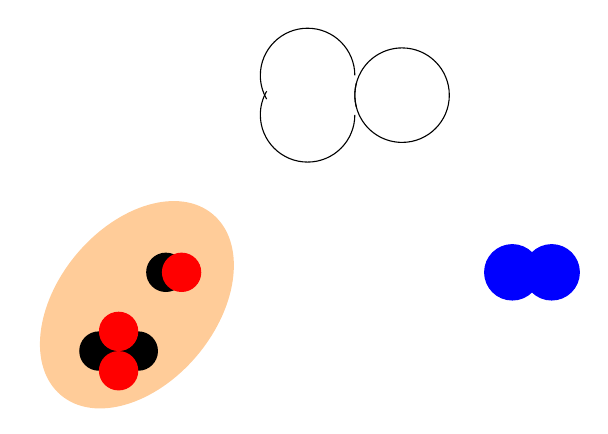
\begin{tikzpicture}		
		\fill[orange, fill opacity=0.4] (0.6,0.2)[rotate = 50] ellipse (1.5 and 1.0);
		
		\fill[black] (0.25, 0) circle (0.25);
		\fill[black] (-0.25, 0) circle (0.25);
		\fill[red] (0, 0.25) circle (0.25);
		\fill[red] (0, -0.25) circle (0.25);
		
			
		\fill[black] (0.6, 1.0) circle (0.25);
		\fill[red] (0.8, 1.0) circle (0.25);
		
		
		%\filldraw [blue] (2,2) -- (2,3) -- (3, 3) -- (3, 2) -- (2,2);
			
		\draw (3,3) arc (0:-210:0.6);
		\draw (3,3.5) arc (0:210:0.6);
		
		\draw (4.2,3.25) arc (0:-195:0.6);
		\draw (4.2,3.25) arc (0:195:0.6);
		
		
		\filldraw[blue] (5, 1) circle (10pt);
		\filldraw[blue] (5.5, 1) circle (10pt);
		
		
		%\draw (4, 4.5) arc(0:-300:0.6)  ;
		
		%\filldraw [green] (3, 3) circle (0.05) ;
		%\filldraw [blue] (4, 4.5) circle (0.05) ;
		
	\end{tikzpicture}
\end{center}

	\caption[Clustered $\mathrm{{}^{6}Li}$ nucleus]{Artistic representation of a clustered $\mathrm{{}^{6}Li}$ nucleus. The nucleus covers a two cluster system with an $\alpha$ particle and a deuterium as its constituencies.  }
	\label{fig:microscopical_cluster}
\end{figure}


An example of clustering is given with the $\mathrm{{}^{6}Li}$ nucleus depicted in Figure \ref{fig:microscopical_cluster}. With this picture, it is observed how the number of interacting bodies has decreased from 6 nucleons to 2 clusters: the  $\mathrm{{}^{4}He}$ and deuterium nucleus.  \\

Additionally, it is said that the $\alpha$ particle and the deuterium nucleus are the core and the valence clusters respectively. This classification is analogous to the core and valence electrons used in atomic physics. In particular, the core corresponds to the $\alpha$ particle cluster since it has more nucleons than the valence cluster which is the $d$ nucleus.  \\

On the other hand, in order to give this kind of models physical significance, selected interactions between clusters are introduced. The $NN$ and $NNN$ forces are standard examples of such needed interactions. In addition, since the constituents usually have many nucleons, extended object parameters like mass and charge density distributions may be encountered. \\

The mass and nuclear density of the nuclei can be modeled as a Woods-Saxon distribution as follows:

\begin{equation} \label{eq:micro_density}
	\rho(r) = \frac{\rho_0}{1 + \exp{\left(\frac{r - R}{a}\right)}}.
\end{equation} 

With folding.

\begin{equation}  \label{eq:micro_folding}
	\int \int \rho(r_1) \rho(r_2) dr_1 dr_2. 
\end{equation}


A more detailed survey on cluster models \cite{beck_2012}.

Microscopical cluster light nuclei \cite{freer_horiuchi_kanada-enyo_lee_meisner_2018}.

Alpha-cluster alpha-closed shell + Woods Saxon potential  \cite{bai_ren_2018}.

Shell model \cite{dong_wang_michel_ploszajczak_2022} two center shell model $\Ofusion$ \cite{tazawa_1974}

Multicluster $\Cfusion$ (3$\alpha$) \cite{dufour_descouvemont_1997}

Hartree-Fock $\Ofusion$ \cite{simenel_keser_umar_oberacker_2013}

Break up effects (four -five body model)\cite{shubhchintak_descouvemont_2022}

Linear chain (Molecular dynamics) \cite{baba_taniguchi_kimura_2022}

\section{Matrix models}  \label{sec:matrixModels}

The matrix models permit the modeling of resonances with an appropriate fitting of free parameters. In particular, the main formalism in this approach is the R-matrix model \cite{lane_thomas_1958} and a more recent review \cite{descouvemont_baye_2010}. \\

Additionally, this alternative models have the advantage that they are compatible with numerical solutions for the wave functions. For example, they use basis functions which serve for mesh generation, which is a critical process in approximating numerically the Schrödinger equation. \\

On the other hand, there are matrix models with no free parameters. For example, the K-matrix model predicts the cross sections without including the channel radius, which is an arbitrary parameter required in the R-matrix calculations \cite{humblet_1990}. \\

This method is also compatible with the Trojan hourse method subbarrier thresholds \cite{mukhamedzhanov_shubhchintak_bertulani_2017}. \\

Finally, there is more than a single parametrization for matrix models \cite{brune_2002}. Usually the alternative formulations surge from the need to express the parameters of the model in order to facilitate the imposition of boundary conditions.  

\subsection{Calculable R-matrix} \label{sub:rmatrix_calculable}

The broad idea of this approach is to parametrize the scattering states of system.  The model includes free parameter $a$ which is called the radius channel. This serves as an estimated value such that at radius $r > a$ the electromagnetical interaction becomes relevant, which is where the radiative region is located. In contrast, in the interior region, with $r < a$, the nuclear force is the dominant interaction. \\

Additionally, boundary conditions are added as an external input. Recall that at the boundary, where $r = a$, the solution to the logarithmic derivative of the Schrödinger equation is imposed to be continuous since this condition implies simultaneous continuity on both the wave function and its first order derivative. Then, an non-dimensional quantity $f$, which is closely related with the logarithmic derivative, is introduced and it is defined as \cite{iliadis_2015}:

\begin{equation}\label{eq:rmatrix_f}
	f = a\left.u(r) \frac{du(r)}{dr}\right|_{r = a}.
\end{equation}

With the channel radius defined, the value of $f(r = a)$ is fixed as a boundary condition, which is usually referred as $B$.  Then, these parameters are also considered as free since they are adjusted. This value allows to define an specific parametrization of the variables of the reaction. \\

Since the formulation of the R-matrix is strongly inspired by the modeling of resonant reactions, a natural starting point is the Breit-Wigner approximation. Particularly, when angular momentum $l$ is considered, the cross section associated to a single resonance is expressed as:

\begin{equation}  \label{eq:rmatrix_breitWigner}
	\sigma = \frac{\pi}{k^2} \sum_{l} \frac{1}{2l + 1} \frac{\Gamma^{(1)}_{l} \Gamma^{(2)}_{l} }{(E - E_l)^2  + \Gamma^2_l }, 
\end{equation}

where $k$ is the wave number, $E_l$ is the energy peak,  $\Gamma^{(1)}_{l}$ and $\Gamma^{(2)}_{l}$ are the partial widths for the reactant species and $\Gamma$. summed and then averaged corresponds to the total width, which is defined as: 

\begin{equation}  \label{eq:rmatrix_totalWidth}
	\Gamma_l = \Gamma^{(1)}_{l} + \Gamma^{(2)}_{l}. 
\end{equation}

Additionally, an average over the sum of each contribution related to a particular value of $l$ is performed by introducing the $(2l +1)$ divided factor. \\

Within the Breit-Wigner formalism, the energy peak and the width can be expressed terms of $f$. Before introducing the exact form of the relation, it is necessary to define additional variables that would help to expressed the aforementioned physical observable quantities.  \\

One of such variables is the penetration factor $P_l$, which is defined as: 

\begin{equation}  \label{eq:rmatrix_penetrationFactor}
	P_l = \frac{a}{(k_1 f(r = a ))^2 + \left(k_2 \left.\frac{df}{dr}\right|_{r = a} \right)^2 }.
\end{equation}

This parameter is useful when expression the reaction width as: 

\begin{equation}   \label{eq:rmatrix_width_penetration}
	\Gamma_l = 2CP_l\gamma^2_l,
\end{equation}

where $\gamma$ is another variable named as reduced width,  which is defined as: 

\begin{equation}   \label{eq:rmatrix_reducedWidth}
	\gamma^2_l =C P_l\gamma^2.
\end{equation}

On the other hand, the energy peak is expressed in terms of $f$ as: 

\begin{equation}  \label{eq:rmatrix_energyPeak}
	E_l =  C P_l.
\end{equation}

The previous expressions used the fact that $f$ can be expanded in power series as following: 

\begin{equation}   \label{eq:rmatrix_f_powerSeries}
	f(r) = f(a) + \left.\frac{df}{dr}\right|_{r = a} (r - a) +  \frac{1}{2!} \left.\frac{d^2f}{dr^2}\right|_{r = a} (r - a )^2  ... \ .
\end{equation}

Then, equations \ref{eq:rmatrix_width_penetration},     \ref{eq:rmatrix_reducedWidth} and \ref{eq:rmatrix_energyPeak} where obtained by approximating $f$ up to first order in the expansion.\\

Actually, a convenient rearrangement of terms can converge to the definition of a special variable, which is called the R-matrix, as: 

\begin{equation}  \label{eq:rmatrix_definition1}
	R= \sum_k {\frac{\gamma_{k} \gamma_{'k}}{E - E_k}}, 
\end{equation}

where $\gamma_{k} $ and $\gamma_{'k}$ are quantities which would play an analogous, but not necessary exact, role to reduced widths. Similarly, the R-matrix poles $E_k$ are associated but not always equal to the energy peaks. The connections of the last mentioned parameters with $f$ are equivalent to those presented in equations \ref{eq:rmatrix_width_penetration},     \ref{eq:rmatrix_reducedWidth} and \ref{eq:rmatrix_energyPeak}.   \\

The R-matrix can be interpreted as a convenient tool for synthesizing variables of the reaction picture, which now includes the asymptotic effects of the Coulomb potential in a unified formalism. \\

With this picture at the resonance level being settled, it is necessary to consider the asymptotic behavior far from the interaction center. Coulomb factors give the asymptotic behavior of the wave function at $r > a$, which is expressed as \ref{eq:scattering_Schrodinger_radial_solution_coulomb}. Then, the $f$ factor is given by: 

\begin{equation}   \label{eq:rmatrix_f_Coulomb}
	f(r) = k_1\frac{dH^{+}}{dr}  + k_2 \frac{dH^{-}}{dr}.
\end{equation}

With the last expression into account, is now possible to define the connections between the observed, in the experimental sense, and their correspondent R-matrix parameters. Before that, it is critical to remark that Coulomb interaction inclusion in the R-matrix formalism implies the need of defining a factor $S_l$ as:

\begin{equation}   \label{eq:rmatrix_shiftFactor}
	S_l= K P_l\gamma^2_l,
\end{equation}

Then, a pole of the R-matrix $E_\lambda$ is expressed as: 

\begin{equation}  \label{eq:rmatrix_energyPole}
	E_\lambda =  E_l - \Delta, 
\end{equation}

where the energy shift is given by: 

\begin{equation}  \label{eq:rmatrix_energyShift}
	\Delta = k_1 S_l.
\end{equation}

At this point, it is worth to be noticed that $S_l = 0$ for the case of uncharged reaction pictures. Then, for such situations, $E_\lambda = E_l$ holds and therefore there the energy pole and the actually observed energy peak are equivalent. However, within the R-matrix formalism, a shift appears when relating these two energy like terms in therms of $S_l$, which is frequently referred as the shift factor. \\

Additionally, the reaction reduced $\gamma^2_\lambda$ of the R-matrix model  with is defined as:

\begin{equation}   \label{eq:rmatrix_reducedWidth_formal}
	\gamma^2_\lambda =C P_l\gamma^2 + C_2 \Delta.
\end{equation}

Notice that the width has been also corrected by the shift factor. \\

However, the R-matrix has not a unique parametrization for the quantities associated with observables. In particular, it is possible to simplify the last expressions by imposing: 

\begin{equation}  \label{eq:rmatrix_spacialboundaryCondition}
	B = f(r = a). 
\end{equation}

Then, with this parametrization, $\Delta = 0$ and thus the formal and width parameters become equivalent. Naturally, equation \ref{eq:rmatrix_spacialboundaryCondition} is usually  the preferred for R-matrix calculations. \\

The last introduction of the R-matrix for was based on the requisite of narrow resonance. However,  is possible to describe reactions with multiple channels and to generalize the assumptions made in the Breit-Wigner formalism with the same R-matrix definition. Particularly, extended resonances and non-resonant behavior can be also analyzed withing this theoretical framework.\\

Further approaches in the context of the R-matrix have different forms depending on the inclusion of effects of channels and spins. The first approximation is given by considering a single channel. Additionally, spin effects and the related formulae are included in the R-matrix formalism. Angular momentum and parity conservation can be included within R-matrix calculations. \\

As multiple incoming and outgoing states are treated, it is necessary to define a connection of the R-matrix with the S-matrix, which ultimately permits the interpretation of the physics of the scattering process. The previous requisite motivates the introduction of a matrix which contains the details of scattering physics. This R-matrix is defined as:

\begin{equation}  \label{eq:rmatrix_elements}
	R_{cc'} = \sum_k {\frac{\gamma_{ck} \gamma_{c'k}}{E - E_k}}, 
\end{equation}

where $c$ and $c'$ are the labels for the entrance and exit channels, $k$ is an index through all the poles with energy $E_k$. $\gamma_{ck}$ and $\gamma_{c'k}$ are the widths of the processes involving both the entrance and exit channels with respect to the pole considered. \\

All the previous parameter are dependent on both the channel radius  $a$ is a free parameter.  \\

It is worth to be noticed that although the widths and energies of equation \ref{eq:rmatrix_elements} could be interpreted as being related with the actual widths or energy peaks of resonances, this is not always the case. In fact, there is a consistent shift between the measured widths and energy peaks of resonances and the $E_k$ and $\gamma$ like parameters encountered in the definition of the R-matrix.  \\

With these parameters being established, it is now possible to introduce the connection between the R-matrix and the S-matrix. Particularly, this is modeled by incorporating a new variable called the collision matrix $O$. \\

Guess: They can be deduced from calculable R-matrix
but fitted with phenomenological R-matrix

Picture A: Scattering picture ?
	-	Potential 
	-	Microscopical ...
	
Picture B: Phenomenological by fitting 
	-	 Raw fitting 
	-	R-matrix more sophisticated 

Matrix

R-matrix has a connection with the collision matrix, which is closely related with the S-matrix. 

S-matrix has already a connection with cross section. 

With the difference that $a$ plays some role here. 

Channels unified parts with different contribution for a same reaction or resonances. 

Does R-matrix serve to deduce the resonant levels? 

Or a potential is needed with bounded solution to the Schrödinger equation.  

The R-matrix approach serves as a framework for modeling several kind of reactions. 

Boundaries or not boundaries. Related with wavefunction 

Exchange reaction: (DWBA)
Proton capture reaction: (First order perturbation theory + radiative transitions + spin implementation + .. )

WKB: potential to the wave function: 

Effective field theory: Low energy $L_{QCD}$. 
QCD is SU(3). However, this is unnecessary sophisticated and effective interactions within nuclei can be introduced with fermionic fields. 

Chiral and additional topological effects to be used as the description of states.

Difference between state and element of the periodic table. A nuclear state consist of an object associated with a pair of A, Z and also  with a certain energy and additional quantum number values.

From the microscopical point of view, there are aspects of the microscopical world to reduced a N-body calculation to  clustering or molecular calculations (examples)

Guess: SU(2) of flavor might be here. Mesons can be mediators. 

The advantage is that all the quantum field theory machinery is available.

Also lattice quantum field theory could be introduced here if convenient and other stochastic methods that use, for instance, Monte Carlo methods. 

The sum is over levels and the elements are parameterized as channels.  \\

Resonances arrives from poles. Deviations from Breit-Wigner resonance prediction. A description on the physical consideration of poles in the scattering (S-matrix) is given in \cite{ramirezjimenez_kelkar_2018}. \\

Applications of the R-matrix formalism to specific reactions:

In primordial nucleosynthesis \cite{desouza_iliadis_coc_2019} big-bang 3He and several reactions \cite{sparta_pizzone_bertulani_hou_lamia_tumino_2020}. \\

Bayesian fitting methods \cite{odell_brune_phillips_2022}.

Lithium deuterium capture \cite{grineviciute_lamia_mukhamedzhanov_spitaleri_lacognata_2015}. \\

10B proton non-radiative \cite{kolk_macon_deboer_anderson_boeltzig_brandenburg_brune_chen_clark_danley_et_2022} and similarly \cite{sieverding_randhawa_zetterberg_deboer_ahn_mancino_martinez-pinedo_hix_2022}. 10B radiative and resonances in 11C inverse kinematics \cite{kaur_guimaraes_zamora_assuncao_alcantara-nunez_delara_zevallos_ribeiro_lichtenthaler_pires_et_2022}.

Alpha capture reactions of carbon \cite{schurmann_gialanella_kunz_strieder_2012}.  Hybrid potential/R-matrix \cite{sparenberg_2005}. \\ 13C alpha capture and 16O determination \cite{prusachenko_bobrovsky_bondarenko_bokhovko_gurbich_ketlerov_2022}.

Proton capture carbon \cite{burtebaev_igamov_peterson_yarmukhamedov_zazulin_2008} for C12 and \cite{chakraborty_deboer_mukherjee_roy_2015} for C13 and \cite{genard_descouvemont_terwagne_2010} for the same reaction. \\

15N capture in \cite{barker_2008} and 14N in \cite{angulo_champagne_trautvetter_2005}. also on 14N proton capture \cite{formicola_imbriani_costantini_angulo_bemmerer_bonetti_broggini_corvisiero_cruz_descouvemont_et_2004}.

\subsection{Phenomenological R-matrix} \label{sub:rmatrix_phenomenological}

Obtaining the R-matrix from the Schrödinger equation is usually a complex task. In particular, when the number of channels grow, the R-matrix functions are more challenging to compute. This complexity issue motivates the need of an approach which leans to simplifying the formalism.  \\

Instead of solving the Schrödinger equation, it is possible to obtain specific formulas that account for the R-matrix  behavior up to a certain degree of certainty.  \\

One example of an approximation used in the context of phenomenological R-matrix is the single channel approximation. This allows to simplify the definition of the matrix to: 

\begin{equation} \label{eq:rmatrix_simplified }
	R= \frac{\gamma^2}{E - E_r},
\end{equation}

where $\gamma$ and $E_r$ are the total width and the energy pole parameter respectively. \\

With the previous approximation taken into account, it is possible to express the penetration factor parameter $P(E)$ as:

\begin{equation} \label{eq:rmatrix_penetrationFactor_coulomb}
	P= \frac{\Gamma}{F_l^2 + G_l^2},
\end{equation}

where the functions $F_l = F_l(ka)$ and $G_l = G_l(ka)$ are the Coulomb functions evaluated at a particular $\rho = ka$. \\

In addition, a complementary parameter $Q$ is defined in terms of the derivatives of the regular and irregular Coulomb functions, which are defined as $F_l'(ka) = dF/dr(ka)$ and $G_l'(ka) = dG/dr(ka)$ respectively. The expression for the $Q$ factor is given by: 

\begin{equation} \label{eq:rmatrix_QFactor}
	Q = \frac{\Gamma}{F_lG_l' + G_lF_l'}.
\end{equation}

It is possible to estimate the phase shift with the R-matrix formalism. There are two main contributions: the background, which is usually non-resonant, and the resonant. \\

The particular expression of the phase shift depends on terms to be computed. Usually, this is approximated by:

\begin{equation}  \label{eq:rmatrix_phaseShift}
	\delta = \delta_{\mathrm{HS}} + \delta_R,
\end{equation}

where $\delta_{\mathrm{HS}}$ and $\delta_R$ are hard sphere and resonant contributions to the phase shift. \\

Then, with all the variables considered, an empirical formula obtained from the R-matrix formalism is given by:

\begin{equation} \label{eq:rmatrix_sfactor}
	S(E) = S_r \frac{\Gamma^2/4}{(E-E_r + \Delta)^2 + (\Gamma/2)^2}.
\end{equation}

\subsection{K-matrix} \label{sub:kmatrix}

There is also the K-matrix model as an alternative of the R-matrix model \cite{humblet_1990}. The advantage of this model with respect to the R-matrix is that the K-matrix does not include the channel radius as a free parameter.  Alternative formulation of R-matrix \cite{brune_2002}. \\

The parametrization is identical to the R-matrix case for most of the steps. However, there are critical differences in this formalism that make it dependent on no free parameter dependent. 

\section{Potential models} \label{sec:potentialModels}


Since nuclear force is an interaction which is far from being analytically parametrized, or even closely parametrize, models with effective interactions, which have associated potentials, are of substantial interest when modeling nuclear reactions.  \\

The main approach is to consider nuclei as objects sensible to a common interaction, which is estimated by an effective potential, generated by the reactant nuclei. Exact shapes of such potentials are given in section \ref{sub:potential_effective}. Then, as it is explained in section \ref{sub:potential_calculations}, calculations are performed to obtain cross sections, and then astrophysical S-factors. Additionally, potentials can be modified to include features like folding and non-locality. Further details about these two aspects are given in sections \ref{sub:potential_folding} and \ref{sub:potential_nonlocality} respectively.

\subsection{Effective potentials} \label{sub:potential_effective}

These interactions are also modeled by effective potentials which account qualitatively for the nature of the underlying physics behind the nuclear reactions. In particular, different kind of potentials offer a particular shape of the interaction which make them suitable for the modeling of concrete reactions.

\subsubsection{Electromagnetic standard potential} \label{sub:potential_effective_EM}

The effective interaction between nuclei is referred as a composite effect of the electromagnetic and nuclear interactions.  \\

The first interaction is considered due to the electromagnetic repulsion between the nuclei. In a first approach, the  substructure of the nuclei is ignored. Then, nuceli charged cloud is modeled as uniformly charged sphere. Therefore, the corresponding potential is given by:

\begin{equation} \label{eq:potential_EM}
	V_{\mathrm{EM}} = 	\left\{\begin{array}{l}
		\begin{split}
			\frac{Z_1Z_2e^2}{4\pi\epsilon_0R}\left(\frac{3}{2} - \frac{r^2}{2R^2}\right), \quad &r \le R \\ 
			\frac{Z_1Z_2e^2}{4\pi\epsilon_0r}, \quad &r > R	
		\end{split}
	\end{array}\right.
\end{equation}

Initially, the potential descends as a parabolic term in the interior region of the sphere and then it decays in the familiar $1/r$ form outside of the sphere. 

\subsubsection{Empirical potentials} \label{sub:potential_effective_empirical}

Secondly, in order to account for the nuclear force, an short-distance attractive potential is needed to be included. However, unlike the electromagnetic interaction, nuclear potentials might not be deduced  in a closed and fundamental form such as the expression given in \ref{eq:potential_EM}. Consequently, these  potentials are usually phenomenological and account for specific purposes. In fact, there is a an extent list of potentials available in literature which are used for modeling the interactions of different kind of reactions. \\

For instance, in a first approximation, there is the step potential.

\begin{equation} \label{eq:potential_squareWell}
	V_{\mathrm{SqW}} = -V_0\theta(r).
\end{equation}

Gaussian exponential: 

\begin{equation} \label{eq:potential_gaussianExponential}
	V_{\mathrm{GE}}(r) = - V_0 \exp{(-\alpha r^2 )}.
\end{equation}

This is useful when considering $\alpha-\alpha$ interactions.  \\

Some potentials can be constructed on top of simpler potentials. \\

Double exponential:

\begin{equation} \label{eq:potential_doubleExponential}
	V_{\mathrm{DE}}(r) = - V_0 \left(e^{\alpha_1 r} + e^{\alpha_2 r} \right)^{-1}.
\end{equation}

It modifies the exponential degree one by adding an additional term with $\alpha_2$ as the new parameter. \\

Cluster potential:

\begin{equation} \label{eq:potential_cluster}
	V_{\mathrm{CL}}(r) = - V_0 \exp{(-\alpha r^2 )} + V_1 \exp{(\beta r)}.
\end{equation}

It adds the Gaussian potential to a first order exponential decaying term, which is parametrized with the variable $\beta$. \\

Yukawa potential  which includes screening effect due to a heavy mass exchange boson.

\begin{equation} \label{eq:potential_Yukawa}
	V_{\mathrm{Y}} = -\frac{c}{4\pi\epsilon_0}e^{-\mu r}.
\end{equation}

It is seen as a mixture between the exponential and a Coulomb like potential. In fact, this potential was used as an estimation for the primitive nuclear interactions, which was possible due to exchange of some mesons mediators like the pion. \\

Additionally, there are potentials in where the nuclear and electromagnetic contributions are not necessarly added. \\

This is the case of the potential of Yakovlev et. al model \cite{yakovlev_beard_gasques_wiescher_2010} which consists of an estimation of the potential that is similar to the parabolic potentials with free parameters that attempt to account for the effects of the nuclear and electromagnetic interactions.  \\

\begin{equation} \label{eq:potential_Yakovlev}
	V_{\mathrm{YAK}} = 	\left\{\begin{array}{l}
		\begin{split}
			E_c\left(3 - \frac{r^2}{R_c^2}\right), \quad &r \le R_{c1} \\ 
			\frac{Z_1Z_2e^2}{r}, \quad &r > R_{c1}	
		\end{split}
	\end{array}\right.
\end{equation}


proton capture review $\mathrm{{}^{2}H}$, $\mathrm{{}^{6,7}Li}$, $\mathrm{^{12, 13}C}$ reactions (two-cluster potential model, exponential 21, exponential2 + Young's scheme) + poly parametrization \cite{dubovichenko_dzhazairov-kakhramanov_2012}

7Be radiative capture(exponential2 + Asymptotic normalization coefficients) \cite{tursunov_turakulov_kadyrov_blokhintsev_2021}

Cross section deduced potential  $\Cfusion$ and $\Ofusion$ reactions (exp(11)-1 potential approximated to exp(-1) empirical potential + Liquid drop radius )\cite{bass_1977} Review nuclear potentials heavy-ion reactions (Woods-Saxon and double folding potentials (SPP) + empirical potentials  + mean field model Skyrme Hartree - Fock) + poly6 + polyfrac for potential barriers \cite{nandi_swami_gupta_kumar_chakraborty_manjunatha_2022}

\subsubsection{Woods-Saxon potentials} \label{sub:potential_effective_woodsSaxon}

In order to the potential to be more realistic, a Woods-Saxon potential consider a smooth behavior.

\begin{equation} \label{eq:potential_WoodsSaxon}
	V_{\mathrm{WS}}(r) = \frac{-V_0}{1 + \exp  \left({\frac{r-R}{a}}\right)},
\end{equation}

where $V_0$ represents the potential depth, $a$ the parametrization and $R$ a computed radius which is defined as: 

\begin{equation} \label{eq:potential_WoodsSaxon_radius}
	R = r_0(A_1^{1/3} + A_2^{1/3}).
\end{equation}

Further details about capture reactions (potential model Woods-Saxon + spin-orbit coupling + ANC + SF) with single-particle states is given by \cite{huang_bertulani_guimaraes_2010}. \\

Coupled channels  E1, M1 and E2 transitions (Woods-Saxon + spin-orbit coupling + spectroscopic factor) \cite{bertulani_1996}

9Be radiative capture. Mostly E1 transition.  (modified Woods-Saxon + spin-orbit + SF + ANC) \cite{kabir_nabi_2021}

11C radiative capture (modified Woods-Saxon + spin orbit coupling)\cite{kabir_irgaziev_nabi_sagheer_2022}

On the other hand, it is relevant, specially at low energies, the inclusion of angular momentum effects in the potential. In order to account for that effect, there is the potential with angular moment. \\

\begin{equation} \label{eq:potential_WoodsSaxon2}
	V_{\mathrm{WS}} = -V_0 f(r),
\end{equation}

Fermi-Dirac distribution like term: 

\begin{equation}  \label{eq:potential_WoodsSaxon2_fermiDirac}
	f(r) = \frac{1}{1 + \exp {\left(\frac{r- R}{a}\right)}}.
\end{equation}

Surface Fermi-Dirac, which is related to the derivative, is a distribution like the following term: 

\begin{equation}  \label{eq:potential_WoodsSaxon2_surfaceFermiDirac}
	f_{\mathrm{S}}(r) = \frac{\exp{\left(\frac{r - R}{a}\right)}}{\left(1 + \exp {\left(\frac{r- R}{a}\right)}\right)^2}.
\end{equation}

And the generalized Woods-Saxon potential is now expressed as: 

\begin{equation} \label{eq:potential_GeneralWoodsSaxon}
	V_{\mathrm{GWS}} = -V_0 f(r) - V_1 	f_{\mathrm{S}}(r).
\end{equation}

In addition to the Woods-Saxon and generalized Woods-Saxon potential, it is possible to include cut-off inclusion for numerical implementations. \\

As an example, a Woods-Saxon potential can be solved analytically with $l = 0$ with cut off procedure \cite{salamon_baran_vertse_2016}. \\

coupled channels and modified energy dependent diffuseness parameter for modified Woods-Saxon \cite{singh_sukhvinder_kharab_2013A} \\


In order to make the model more general, some parameters like $V_0(E)$ and $a(E)$, are made energy dependent. Recurrent formulas are reported in literature for this parameters which help to effectively.

\subsubsection{Spin orbit contribution} \label{sub:potential_effective_spinOrbit}

As it was anticipated with the description of the nuclear shell model in section \ref{ssub:nuclearShellModel}, spin orbit coupling is commonly relevant when performing nuclear physics calculation. Specially, it is noticiable at low energies. \\

In order to account for that effect, there effective potential of the interaction shall be modified by accounting for the angular momentum coupling. \\

 In the context of nuclear reactions, this coupling consists of an extra interaction between the relative orbital angular momentum $\hat L$ of the interacting nuclei and the spin $\hat S$ of the nuclei. \\

The exact form contribution to the potential associated with this effect is expressed as:

\begin{equation}  \label{eq:potential_spinOrbit}
	V_{\mathrm{SO}}(r) = k\langle L \cdot S \rangle  \frac{1}{m_{\pi}r} \frac{d}{dr} V(r),
\end{equation}

One of the consequence of spin orbit coupling, is the introduction of a first derivative term. It is quite remarkable that the result of equation \ref{eq:potential_spinOrbit} is valid for any central potential.  \\

Now, in order to compute the   $  \langle L \cdot S \rangle$ coupling, a common approach is to proceed by expanding the operator  $\hat J^2 = (\hat L + \hat S)^2$ and finding the coupling. Then, the resulting term is expressed as: 

\begin{equation}  \label{eq:potential_spinOrbit_LSexpansion}
	\langle L \cdot S \rangle =  \frac{1}{2}[j(j+1) - l(l+1) - s(s+1)].
\end{equation}

Is not always the case, specially for large heavy nuclei, that the LS coupling is the ideal one to be used. Instead, some models include the $jj$ coupling. This alternative approach defines as the good quantum numbers the total angular momentum of the reactant nuclei.

\subsubsection{Optical potentials} \label{sub:potential_effective_optical}

Optical model (Modified Woods-Saxon energy dependent) $\mathrm{{}^{12}C}$ with $A = 6$ projectile reactions + double folding São Paulo (SPP)  and double folding cluster model dynamic polarization potential + poly2 empirical formulas \cite{amer_penionzhkevich_2021}. \\

Hill-Wheeler approximation for transmission probability and applications in fission reactions \cite{hill_wheeler_1953}.

Hill-Wheeler approximation  application to $\mathrm{{}^{11}Li + {}^{12}C}$ reaction + optical model + Wong's formula  \cite{esbensen_2012}.
 
Coupled channels + optical potential +  polarization +  Hill-Wheeler approximation  +  WKB approximation \cite{cardenas_canto_donangelo_hussein_lubian_romanelli_2002}.

\begin{equation}  \label{eq:potential_Optical}
	V(r) = V_R(r) + iW_R(r),
\end{equation}

where $V_R(r)$ and $W_R(r)$ correspond to the real and imaginary parts of the potential respectively. Usually, the real term contains the relevant electromagnetic and nuclear interactions while imaginary term accounts for absorption to inelastic channels. \\

In fact, this model is referred as optical since imaginary term is used in optics to model the damping effect of light when entering a dissipation medium. Analogously, in the optical model, the imaginary term counts for a dismissal of the probability of a particular process due to absorption to inelastic channels. \\

Optical energy dependent model (parabolic approximation with analytical cross section) \cite{singh_sukhvinder_kharab_2013B}

\subsection{Calculations}  \label{sub:potential_calculations}

The potentials just introduced are useful for the calculation of cross sections and, therefore, S-factors. The connection between potentials and cross sections depends on the kind of reaction to be modeled. In the general approach, cross sections are directly computed form wave functions,  which are numerically estimated from the numerical solution of the Schroödinger equation. \\

\subsubsection{WKB approximation} \label{ssub:potential_calculations_WKB}

Fusion cross section calculations using the WKB approximation method are closely related with the Barrier penetration model (BPM). In this model,  the factor $\Phi(E)$, which was introduced in section \ref{sub:tunnelingPhenomena} and in equation \ref{eq:WKB_definition}, is calculated for the effective potential, which consists of the sum of the nuclear, electromagnetic and centrifugal terms. The last term is associated with an specific $l$ value. Then, it is possible to compute the transmission coefficient $T_l$ for each value of $l$ as it is given by \cite{koyuncu_soylu_2018}:

\begin{equation} \label{eq:potential_WKB_transmission}
	T_l =  \frac{1}{1 + \exp ({\Phi(E)} )}.
\end{equation}

Some authors calculate $\Phi(E)$ by considering a change in the centrifugal term of the potential $V_{\mathrm{Cent}}$ in order to introduce a term consistent with the connection formulas of the WKB formalism. It particular, accordingly to this approach, the centrifugal contribution to the potential shall be modified as: 

\begin{equation} \label{eq:potential_WKB_modified_centrifugal}
	V_{\mathrm{Cent}} = \frac{(l + 1/2)^2 \hbar^2}{2\mu r^2}.
\end{equation}

Subsequently, a summation over all the values of $l$ is performed until convergence is achieved. It turns out that there is a direct relation with the fusion cross section and the referred sum as it is expressed by \cite{koyuncu_soylu_2018, nobre_chamon_gasques_carlson_thompson_2007}:

\begin{equation} \label{eq:potential_WKB_crossSection}
	\sigma = \frac{\pi}{k^2} \sum_{l}{(2l + 1)T_l},  
\end{equation}

where $k = \sqrt{2\mu E / \hbar^2}$ and $\mu$ corresponds to the reduced mass of the reactant nuclei.  \\

It is quite remarkable that the calculation of the cross section of a sophisticated process like the fusion reaction can be reduced to a discrete sum of transmission coefficients. In fact, the expression of equation \ref{eq:potential_WKB_crossSection} does not need to take into account the outcome of the initial or final state. It also, it permits the evaluation of the cross section without considering further details about the structure of the fusing nuclei.  \\

However, the BPM has the main disadvantage that does not account for couplings that might exist among the sub components of the nuclei. In particular, this approach, at it will be detailed later in this work, lens to underestimate the cross-section values for nuclei. In order to overcome this issue, further models, like the zero point motion model (ZPM), are introduced in literature \cite{duarte_gasques_oliveira_zagatto_chamon_medina_added_seale_alcantara-nunez_rossi_et_2015, nobre_chamon_gasques_carlson_thompson_2007}.   \\  

There are ways for simplifying equation   \ref{eq:potential_WKB_transmission}. This is done by introducing the Hill-Wheeler approximation, which states that the transmission coefficient can be effectively estimated as: 

\begin{equation} \label{eq:potential_WKB_transmission_HW}
	T_l =  \frac{1}{1 + \exp {\left ( \frac {2\mu E} {\hbar^2} \right)} }.
\end{equation}

This approximation allows to compute the cross section in a more direct manner, which is simplified to: 

\begin{equation} \label{eq:potential_WKB_crossSection_HW}
	\sigma = \exp{\left( - \frac{2\mu E}{\hbar^2}\right)}.
\end{equation}

Another approximation is given by estimating the potential as a barrier $V_B$ plus a parabolic term as:

\begin{equation} \label{eq:potential_WKB_potential_Wong}
	V(r) \approx V_B + \frac{l(l+1) \hbar^2  r^2 }{2\mu}.
\end{equation}

The previous estimation configures the core of the Wong's approximation. Then, as the potential has been simplified, it is possible to find an analytical solution to the cross section, which is expressed as: 

\begin{equation} \label{eq:potential_WKB_crossSection_Wong}
	\sigma = \left( 1 + \ln{\frac{2\mu E}{\hbar ^2}} \right).
\end{equation}

Additionally, there are empirical alternatives to the calculation of S-factor by introducing additional free parameters. For instance, in the Yakovlev et. al potential model, the S-factor is parametrized in two regions and it uses two free parameters.  The details of this model are going to be introduces, as they given in \cite{yakovlev_beard_gasques_wiescher_2010}. 

For the first region, which consists of energies below the Coulomb barrier $E_c$, the astrophysical S-factor is estimated as:

\begin{equation}  \label{eq:potential_Yakovlev_sfactor_belowBarrier}
	S(E) = S_0 \exp ({\Psi(E)} ),
\end{equation}

with $\Psi(E)$ defined as: 

\begin{equation}  \label{eq:potential_Yakovlev_psiWKB}
	\Psi(E) = 2\pi\eta(E) + \Phi(E),
\end{equation}

where $\eta(E)$ is the Sommerfeld parameter, and $\Phi(E)$ is the wavefunction calculated by the WKB, which is given in equation \ref{eq:WKB_definition} with $m = \mu$, where $\mu$ corresponds to the reduced mass of the colliding nuclei. Further details on the calculation of the last parameter are presented in section \ref{sub:tunnelingPhenomena}. \\

It is worth noticing that $S_0$ corresponds to a free parameter closely related with the S-factor value extrapolation at zero energy. In addition, as it happens usually to free parameters, $S_0$ is determined by fitting the model with experimental data. \\

On the other hand, for the second region, which corresponds to energies above the barrier, the S-factor is given by:

\begin{equation}  \label{eq:potential_Yakovlev_sfactor_aboveBarrier}
	S(E) = S(0) \exp ({2\pi\eta(E)}) \sqrt{\frac{Ec}{E}} \left( 1 + \xi\frac{E - E_c}{E} \right),
\end{equation}

where $\xi$ is the other free parameter which accounts for the deviation from Coulombic behavior of the S-factor.  \\

\subsubsection{Exchange reactions} \label{ssub:potential_calculations_exchange}

Since the form of the reaction is $A(a, b)B$, there are four interacting nuclei and two substeps that account for the global behavior of the reaction. In fact, depending on  $a$ and $b$ nuclei, there are two options the reaction to proceed \cite{xu_takahashi_goriely_arnould_ohta_utsunomiya_2013}. \\

The first option is related with $ a \rightarrow x + b$,  $A + x \rightarrow B$ and happens when $a$ is heavier than $b$. In contrast, the second option has the processes: $a + x \rightarrow b$ and $A \rightarrow B + x$, which are possible if $a$ is lighter than $b$. More details of such steps are presented in section \ref{ssub:exchangeReactions} \\

It is desirable that exchange reaction to be reduced to a transition involving only an incident and outgoing effective nuclei. This is achieved if the pair of reactants $a$ and $A$, as well as the pair of products $b$ and $B$, are considered as composite systems. Hence, the process will be reduced to a $(aA) \rightarrow (bB)$ transitions with $(aA)$ and $(bB)$ being coupled states of aforementioned pairs. The simplest way of coupling reactants and products is by considering their elastic scattering states. \\

In order to compute scattering states, it is required to proceed with solving the Schrödinger equation for the scattering scenario of $aA$ and $bB$ with an adequate potential. Then, the wavefunction for $aA$ and $bB$ scattering, named as  $\phi_c$ and $\phi_c'$ respectively will be computed. \\

Then, with the scattering wavefunctions already calculated, the differential cross section is obtained by:

\begin{equation} \label{eq:exchange_differential}
	\frac{d\sigma}{d\Omega} = \frac{1}{4\pi} K \frac{1}{E E_f} \frac{k_f}{k}\frac{m^2_B}{m^2_A} \sum_{slj} { \frac{S^2_F}{2s + 1}\sum_{m} |t|^2},
\end{equation}

where $E$ is the center of mass energy and $E_f$ is the final energy.  $CS^2$ accounts for the spectroscopic factor, and $K$ is a constant with value:

\begin{equation} \label{eq:exchange_constant}
	K = 	\left\{\begin{array}{l}
		\begin{split}
			\frac{(2J_B + 1)}{(2J_A + 1)}, \quad &\mathrm{\ stripping} \\ 
			\frac{(2J_b + 1)}{(2J_a + 1)}, \quad &\mathrm{\ pickup}
		\end{split}
	\end{array}\right.
\end{equation}

The last result is consistent with the differentiated reaction mechanisms associated to the stripping and pickup reactions. Particularly, the factor pretends to average over all spin configurations on the channel in where the intermediate nuclei is consumed.  Additionally, $t$ is a term related with the exchange term which is approximated by the distorted Born wave approximation (DWBA). \\

This approach is privileged for exchange reaction calculations. The transition matrix $T^{cc'}$ is expressed as: 

\begin{equation}\label{eq:exchange_matrix}
	T^{cc'} = \langle  \phi_c | \frac{\phi}{r}|  \phi_c' \rangle,
\end{equation}

where $\phi_c $ and $\phi_c'$ are the unbounded wavefunctions for the entrance and exit channels while $\phi/r$ is given in terms of the bounded intermediate state wave function $\phi$ and it is referred as the form factor. \\

The total cross section $\sigma$ associated with a particular state $J^{\pi}$ is given by: 

\begin{equation} \label{eq:exchange_crossSection}
	\sigma = K \frac{1}{E E_f} \frac{m^2_B}{m^2_A} \sum_{slj} { \frac{S^2_F}{2s + 1}\sum_{m} \sum_{l_{c'}} \left|\sum_{l_{c}} T^{cc'}\right|^2},
\end{equation}

where the last summations run with initial $l_{c}$ and final $l_{c'}$ angular momentum indexes respectively. \\

Notice that the previous result shows the picture of a two potential interacting. The expression can be obtained by taken into account the Born series approximation and to apply it for the case that interaction between $A$ with $a$ and $B$ with $b$ is considerable larger than the merging-breaking middle state. \\

The wave is said to be distorted given that it does not correspond to a plain wave, which is a case that is treated in standard Born approximation. Instead,  $\phi_c $ and $\phi_c'$ are solutions to the scattering $A + a \rightarrow A + a$ and $B + b \rightarrow B + b$ quantum mechanical situations. \\
 
\subsubsection{Radiative capture reactions}   \label{ssub:potential_calculations_radiativeCapture}

Given that photons are emitted in these processes, it is essential to model the reaction as the composed effect of  all electromagnetic transitions going from a bounded to a continuum state.  \\

General approach towards radiative capture calculations are given in \cite{goldhaber_weneser_1955}.\\

In fact, each transition is classified depending of its origin and multipolarity. The first criteria distinguish whether the transition has electric or magnetic nature. The second item is related to the order of the contribution in terms of the multipole expansion. For example, E1 corresponds to an electric transition of first, which corresponds to an electric dipole. \\

Since contributions from higher multipolarity decay more rapidly, the most important contributions to the cross section of the process are dipole radiation. Additionally, electric transitions are stronger than magnetic transition in a factor of $c^2/v^2$, which is noticeable given that energies are non-relativistic.

In addition, parity must be considered for each reactant. For example, photon has $\pi = -1$. Therefore, when electric processes are given, the product of initial $\pi_1$ and final $\pi_2$ parties must take into account whether the transition is electric or magnetic. More particularly, the referred product has the form: 

\begin{equation} \label{eq:radiativeCapture_parity}
	\pi_1 \pi_2 = 	\left\{\begin{array}{l}
		\begin{split}
			(-1)^{\lambda}, \quad & \mathrm{E\lambda} \\ 
			(-1)^{\lambda + 1}, \quad & \mathrm{M\lambda}
		\end{split}
	\end{array}\right.
\end{equation}

In the last equation, $\mathrm{E\lambda}$ and $\mathrm{M\lambda}$ denote electric and magnetic transitions with multipolarity $\lambda$. \\

As it happens in all reactions, the total angular momentum is conserved. Then, all the spin, orbital and total  contributions should be considered. With this picture given, it is imperative the use of Clebsh-Gordan coefficients. \\

Effective charge is used in order to compute the terms of the multipole expansion. For electric transitions, this term $Q$ is calculated by:

\begin{equation} \label{eq:radiativeCapture_Electric_charge}
	Q =  \left(\frac{m_a}{m}\right)^{\lambda}q + \left(\frac{m_b}{m}\right)^{\lambda}q',
\end{equation}

where $m_a$ and $m_b$ are the reactant masses, $m$ is the total mass and $\lambda$ represents the multipolarity. \\

On the other hand, in the case of magnetic transitions, the effective charge is replaced by effective magnetic moment.
The term is more intricate than the electric analogous, as it is expressed as: 

\begin{equation} \label{eq:radiativeCapture_Magnetic_moment}
	\mu =  \left(\frac{g_a}{m}\right)^{\lambda}q + \left(\frac{g_b}{m}\right)^{\lambda}q',
\end{equation}

where $g_a$ and $g_b$ are the intrinsic magnetic moments for the reactant nuclei. \\

In the radiative capture reactions, cross sections are computed based on electromagnetic field operators as it is observed by \cite{huang_bertulani_guimaraes_2010}: 

\begin{equation}  \label{eq:radiativeCapture_crossSection}
	\sigma_m = \sum_{k}{\langle k | \mathcal{O} | m \rangle} C_{klm}.		
\end{equation}

More specifically, the cross section expression is given by considering all the monopole terms, as parametrized with the $l$ value, as it is given by: 

\begin{equation}  \label{eq:radiativeCapture_crossSection_l}
	\sigma_m = \sum_{l} C \frac{E^{2l +1}}{(2l+1)!!} B(l), 		
\end{equation}

where $B(l)$ is the reduced factor with effectively contains all nuclear physics potential picture. Its expression is given by:

\begin{equation}  \label{eq:radiativeCapture_reducedFactor}
	B(l) \propto   |{\langle k | \mathcal{O} | m \rangle}|^{2}_{l}.
\end{equation}

It is usual that certain transitions cannot be completely described by equation \ref{eq:radiativeCapture_crossSection}. In order to account for defect, some authors introduce a new constant called spectroscopic factor for each transition such that the total cross section of the process is expressed as: 

\begin{equation}  \label{eq:radiativeCapture_crossSection_SF}
	\sigma = \sum_{m}{{(SF)}_m\sigma_m},		
\end{equation}

where each ${SF}_m$ correspond to the weight of the $m$th transition. \\ 

Usually, this new term is obtained by experimental fitting \cite{kabir_nabi_2021, xu_takahashi_goriely_arnould_ohta_utsunomiya_2013}. However, it is also common to find the spectroscopic factor to be set at $SF_m = 1$ for all transitions \cite{bertulani_1996}.

\subsubsection{Fusion reactions} \label{ssub:potential_calculations_fusion}

Fusions reactions calculations can be done by assuming a barrier penetration model. In this approach, fusing system surpasses the barrier generated by a composite interaction of the reactant nuclei. A summary of the common potentials used for this task is given in section \ref{sec:potentialModels}. \\

Next, the transmission coefficient is calculated. In order to simplify subsequent computations, the WKB approximation offers a comprehensive approach towards handy estimation of the cross sections. The core of the details of this approach is given in section \ref{ssub:potential_calculations_WKB}.

On the other hand, in certain specific cases, specially for heavy nuclei, the barrier penetration model fails to effectively match experimental data. This discrepancy usually occurs due the lack of consideration of nuclei substructure. \\

An example of an alternative approach to BPM is the zero point motion model (ZPM). This model allows the introduction of deformations in the nuclei, as well as couplings to rotational and vibrational states. 


\subsection{Folding} \label{sub:potential_folding}

During the previous sections, mass and charge distributions were not considered in detail. However, with nuclei with higher mass, the intrinsic distribution of the mass and charge gains relevance in the reaction cross section estimation. \\

In particular, mass and charge is usually concentrated at the center of the nuclei and there is a sharp drop of the mentioned variables in the surrounding of the radius. Therefore, it is common to model these distribution with a Woods-Saxon formula, as it is visualized: 

\begin{equation}
	\rho = \frac{\rho_0}{1 + \exp{\frac{r - R}{a}}},
\end{equation}

where the adjustable parameter $\rho_0$ has units of density and $R$, $a$ are model parameters. \\

In order to account for this effect, an initial formula which accounts 

São Paulo \cite{chamon_2007}

\begin{equation} \label{eq:potential_SaoPaulo}
	V_{\mathrm{SPP}} (r) = V_{\mathrm{F}} (r)e^{-4V^2/c^2}.
\end{equation}

\begin{equation} \label{eq:potential_SaoPaulo_speed}
	V^2 = \frac{2}{\mu} \left( E - V_{\mathrm{F}}(r) - V_{\mathrm{C}}(r) \right),
\end{equation}

where the reduced mass is $\mu$, the Coulomb potential is $V_{\mathrm{C}}(r)$ and the folding potential  $V_{\mathrm{F}}(r)$ is expressed as:


\begin{equation} \label{eq:potential_SaoPaulo_folding}
	V_{\mathrm{F}}(r) = \int \int \rho_1(\vec r_1)  \rho_2(\vec r_2) \delta(\vec r - \vec r_1 +  \vec r_2) {d\vec{r}_1}  {d\vec{r}_2}.
\end{equation}

An illustration is planned to appear in Figure \ref{fig:DoubleFolding}.

\begin{figure}[H]
	\begin{center}
	\begin{tikzpicture}		
	\shade[ball color = black,
	opacity = 0.5
	] (-3,0,0) circle (20pt);
	
	
	\shade[ball color = black,
	opacity = 0.5
	] (3,0,0) circle (20pt);


	\fill[black] (-0.25, 4, 0) circle (2pt) ;
	
	\draw[-{Stealth[scale=2]}] (-3, 0, 0) -- (3, 0, 0);
	
	\draw[-{Stealth[scale=2]}] (-3, 0, 0) -- (-0.25, 4, 0);
	
	\draw[{Stealth[scale=2]}-] (3, 0, 0) -- (-0.25, 4, 0);
		
	\draw (0, -0.25, 0) node {$\vec R$};
	\end{tikzpicture}
\end{center}

	\caption[Double folding model calculation illustration]{Double folding model calculation illustration. This figure is under elaboration.}
	\label{fig:DoubleFolding}
\end{figure}

$\Ofusion$ + inelastic and elastic scattering + coupled channels + optical model + folding + M3Y NN effective interaction \cite{hassanain_al_sebiey_2014}.  

Capture reaction review light nuclei (Double folding model + Yukawa-like + spin orbit coupling)\cite{ghasemi_sadeghi_2018}

\subsection{Non-locality}  \label{sub:potential_nonlocality}

Nuclear interactions are affected by an intrinsic quantum mechanical characteristic in which it is not possible to distinguish the incoming to the out coming particle. \\

For example, if a neutron collides with a nucleus and, as a result of a complex process, it emits another neutron, it is not possible to claim that the exiting neutron is the incoming neutron.  This effect is closely related with the so called Pauli non-locality. \\

A first approach to model this effect is by considering the action of the potential $V(r)$ when operating the wave function. A general picture of a non-local potential is given by:

\begin{equation} \label{eq:nonLocality_picture}
	V(r) \psi(r) = U(r) u(\psi) + \int W(r, r') u(\psi'),
\end{equation}

where $u(\psi)$ is related with the wave function, $U(r)$ is the local part of the potential and $W(r, r')$ assumes the role of a kernel term. \\

Notice that the right term involves integration under the primed radius $r'$. This accounts for the fact that non-local potentials are not uniquely defined by the information provided in the point of calculation interest, which is parametrized by $r$ in this case. \\

When the result of equation \ref{eq:nonLocality_picture} is considered, it is possible to conclude that the shape of the Schrödinger will be modified as:

\begin{equation} \label{eq:nonLocality_schrodinger}
	\left(\frac{-\hbar^2 \nabla^2}{2\mu} + V(r)  - E  \right) \psi(\vec r) =   \int W(r, r') \psi(r').
\end{equation}

This modified form is usually named as the integral Schrödinger equation. \\

When it comes to computing equation \ref{eq:nonLocality_schrodinger}, it would be desired to have an equivalent local potential which gives the same results as the non-local potential. \\

In fact, it is possible to find a matching condition to encounter such effective local potential. The precedent was established by the work on non-local approximations for neutron potentials by Perry and Buck \cite{perey_buck_1962}. They state the connection between non-local $V_{\mathrm{N}}$ and local potentials $V_{\mathrm{L}}$ as:

\begin{equation}\label{eq:nonLocality_connection}
	V_{\mathrm{N}} = V_{\mathrm{L}} \exp{\frac{a V_{\mathrm{N}}}{b}}.
\end{equation}

The previous formula gives a way of calculating the desired potential by solving an implicitely defined non-linear equation. In particular, such formula can be encountered in the São Paulo potential definition of equation \ref{eq:potential_SaoPaulo}. \\

The main difference on the São Paulo formulation is the inclusion of the Coulomb potential as part of the local term $U(r)$ . \\

An application to pycnonuclear reactions in neutron stars + strange matter + optical model + Pauli nonlocality + São Paulo  + WKB approximation \cite{golf_hellmers_weber_2009}.\\ 


And, potentials with non-locality are also found in literature. For example, there is the São Paulo potential that accounts for the effect of non-local interactions between the interactant nuclei. \\


p2H radiative capture E1, M1, E2 (exponential 21 + variational method + Young's scheme) \cite{dubovichenko_dzhazairov-kakhramanov_2009}

2Hdp reaction in metallic environments (theoretical and experimental screening effect)  \cite{czerski_huke_heide_ruprecht_2006}

13C radiative capture (modified Woods-Saxon + spin-orbit + SF + ANC) ,  R-matrix treatment for resonant cross section and poly2 empirical formula \cite{kabir_irgaziev_nabi_2020} potential cluster model (exp2 potential + variational method + Young's schemes)
\cite{dubovichenko_2012}


16O fusion two-center shell model with Wood-Saxon potentials (cranking and reduced mass + molecular dynamics) \cite{diaz-torres_gasques_wiescher_2007} \\


\section{Special models} \label{sec:specialModels}

Models which do not fit in the previous categories are presented in this section. Some models use a different approach in a multiple step process, which is the case of the Trojan Horse methods. Others, are based on fundamental aspects of low energy calculations of the strong nuclear interaction, like it is the case for effective field theories. Additionally, there are models which combine advantages of the previously introduced approaches. Such cases are usually referred as hybrid models.

\subsection{Trojan Horse models} \label{sub:special_trojanHorse}

It occurs in a two step reaction process as expressed in:

\begin{equation}\label{eq: special_trojanHorse_reaction}
	A + B \rightarrow a + (b + x)\rightarrow a + (c + d),
\end{equation}

where the first and second steps correspond to the $A + B \rightarrow a + (b + x)$ and $b + x \rightarrow c + d$ reactions respectively. Notice that the $b$ nucleus does not appear as a final product of the reaction as it is consumed in the second step. \\

These two reactions can be related as a double exchange reaction with nucleus $x$ as the intermediate of this process. The identity of this intermediator depends on the nuclei which are reacting. To some extent, $x$ can be modeled as a cluster embedded in the composite $A + B$ nucleus. \\ 

Cross sections for the Trojan Horse method can be given by single and double differential cross section. For the former case, the relevant expression is given by: 

\begin{equation}\label{eq: special_differential_single}
	\frac{d\sigma}{d\Omega} = \sum \sum |\langle a | \hat O | b  \rangle|^2,
\end{equation}

where $\hat O$ is the relevant operator of the process. On the other hand, the double differential operator is given by 

\begin{equation}\label{eq: special_differential_double}
	\frac{d^2\sigma}{d\Omega^2} = \sum \sum \sum \sum  |\langle a | \hat O | b \rangle|^2 |\langle a' | \hat O | b' \rangle|^2,
\end{equation}

where $a$, $'a$ are the initial and $b$, $b'$ the final states pairs respectively. \\

This model is useful for applications with middle heavy nuclei in reactions like $\Cfusion$. The intermediate nucleus is $\mathrm{{}^{4}He}$. \\

The Trojan horse method. Selection of reactions and consideration of the characteristics of the nuclei to be considered in the method \cite{spitaleri_mukhamedzhanov_blokhintsev_cognata_pizzone_tumino_2011}.

\subsection{Effective field theories} \label{sub:special_effectiveField}

Based on effective field theories. The general principle of these theories is that nuclear interactions correspond to low-energy approximate solutions of the physics described in quantum chromodynamics. In particular, direct standard model application at low energies have the restriction of non-convergence of the perturbative theories, and even lack of renormalization. Then, alternative field theories with new appropiate interactions shall be introduced. \\

An example of a Lagrangian $\mathcal{L}$ used within the context of effective field theory is given by: 

\begin{equation} \label{eq:micro_lagrangian_nucleons}
	\mathcal{L} = N^{\dagger}i\hbar\gamma^\mu\partial_\mu N + ... ,
\end{equation}

where the term $ N^{\dagger}i\hbar\gamma^\mu\partial_\mu N$ is closely related with the Dirac kinetic term for a fermion. Particularly, $N$ represents a spinor like corresponding to the nuclei. \\

Now, it is necessary to include the interaction via an introduction of a coupling in equation \ref{eq:micro_lagrangian_nucleons}. This can be done with the coupling Lagrangian  $	\mathcal{L}_{\mathrm{coupling}} $ defined as: 

 \begin{equation} \label{eq:micro_lagrangian_coupling}
 	\mathcal{L} =  C_1 A^\mu j_\mu ,
 \end{equation}

where $C_1$ is the coupling constant, which can be estimated from scattering experiments, $A^\mu $ is a term related with a nucleon field and $j_\mu$ corresponds to the conserved current.  \\

Since these theories are closely related with quantum field theory, it is possible to use diagrams associated with the processes of low-energy nuclear force. In this picture, mediators are mesons like pions. The underlying symmetry can be assumed to be isospin symmetry.  \\

Effective field theory $\dRadiativeCapture$ and three body interaction, M1 is the dominant contribution \cite{sadeghi_khalili_godarzi_2013}

 Halo effective field theory $\BeRadiativeCapture$ reaction + coupled channel implementation + two theories with and without $\mathrm{{}^{7}Be}$ excited core  + E1 and M1 transitions + ANC + Bayesian analysis Metropoli-Hasting algorithm + polynomial empirical formula  \cite{higa_premarathna_rupak_2022}.

\subsection{Hybrid models} \label{sub:special_hybrid}

These models include aspects of potential, microscopical and even R-matrix models. For example, there are models with clustering and effective potentials. \\

Clustering can be included in potentials via the folding introduced in section \ref{sub:potential_folding}. A phenomenological potential, in order to be well characterized, needs to be consistent with microscopical aspects of the nucleus.  Particularly, interactions between clusters can be parametrized with more fundamental microscopical models, which are specialized in treating such interactions. \\

Some models with the R-matrix approach use microscopical calculation to calibrate parameters of the potentials to be used in the calculations. Both models complement each other in a particularly useful manner when resonances are present in middle heavy nuclei fusion reactions. This is a remarkable example since the R-matrix formalism alone is mostly specialized in describing resonances and non resonant behavior of light heavy nuclei. On the other hand, potential or microscopical model calculation usually account for the non resonant part of fusion reactions. \\

\section{Empirical formulas} \label{sec:empiricalFormulas}

And some empirical formulas can be given to approximate the behavior of the S-factor directly. These formulas focus on reproducing the form of the S-factor energy curve rather than performing computations to deduce cross sections.

\subsection{Interpolations} \label{sub:empirical_interpolation}

Non-resonant reactions S-factors can be calculated with polynomial interpolations and fits given their overall smooth and monotonic behavior. Each fit can be characterized by an order, which corresponds to maximum degree of a polynomial in the expansion. Then, based on square error minimization, it is possible to estimate the best polynomial coefficients. The astrophysical S-factor can thus be estimated as:

\begin{equation}  \label{eq:empirical_polynomial}
	S(E) = a_0 + a_1E + a_2 E^2 + ... \, 
\end{equation}

where coefficients of the form $a_k$ correspond to the weights of the polynomials of order $k$. \\

Additionally,  there is a exponential expansion that is reported in literature to be useful. 

\begin{equation} \label{eq:empirical_exponential}
	S(E) = \exp{(g_0 + g_1E + g_2E^2 + g_3E^3 + ...)}.
\end{equation}

Notice that the exponential term of equation \ref{eq:empirical_exponential} corresponds to an embedding of the polynomial expansion given in equation \ref{eq:empirical_polynomial}. This procedure is useful when fitting rapid varying S-factor energy curves. \\

When there is a sharp increase on the S-factor at low energies, like it where a pole at $E = 0$,  more generic expansions are used. These approaches modify the classical polynomial interpolation by introducing a Laurent series expansion. An example of such fitting is given by the formula: 

\begin{equation}  \label{eq:empirical_laurent}
	S(E) =\frac{ a_{-1}}{E} + a_0 + a_1 E + a_2 E^2 + ... \ .
\end{equation}

For most of the reactions, $a_{-1} = 0$, since $S(E)$ should be smooth at very low energies. Therefore, the S-factor is  described as a Taylor series expansion as it is shown in equation \ref{eq:empirical_polynomial}. \\

More sophisticated formulas can imply exponential enhancement coefficients due to screening effects. The particularities of these adjustments are presented in section \ref{sub:resultsAnalysisNonResonant}. 

\subsection{Fusion reactions formulas} \label{sub:empirical_fusion}

A formula consistent with the behavior of the S-factor for a  fusion reaction should include the regimes at energies lower and greater the Coulomb barrier. One possible choice is given by introducing a Woods-Saxon like term in order to distinguish the two aforementioned regions. For example, an empirical formula given in  \cite{beard_afanasjev_chamon_gasques_wiescher_yakovlev_2010} relates the S-factor energy dependence as:

\begin{equation} \label{eq:empirical_yakovlev}
	S(E) = \sum_{k=0}^{N} {a_kE^k} + \left(1 + \exp{\left( \frac{E_c - E}{D}\right)}\right)^{-1} \sum_{l=0}^{M} {b_lE^l},
\end{equation}

where $E_c$ and $D$ are quantities related to the Coulomb barrier and the diffuseness parameter of the Woods-Saxon distribution respectively. \\

In order to check that the formula presented in equation \ref{eq:empirical_yakovlev} is consistent with the expected behavior for fusion reactions, it is essential that it gives two different asymptotic behaviors. On the one hand, at the limit of subbarrier energies with $E \rightarrow 0 $, and if $\exp {(E_c/D)} \gg 1$, as it usually happens since $E_c > D$ holds, the right term of the  vanishes and thus the S-factor approaches to: 

\begin{equation} \label{eq:empirical_yakovlev_0}
	S(E) \rightarrow \sum_{k=0}^{N} {a_kE^k}. 
\end{equation}

Where the last expression corresponds to a polynomial interpolation of order $N$. On the other hand, for superbarrier energies, at the limit of $E \rightarrow \infty $, the exponential factor leans to $\exp {(-E/D)} \approx 0$ and then the S-factor is expressed as: 


\begin{equation} \label{eq:empirical_yakovlev_infty}
	S(E) \rightarrow \sum_{k=0}^{N} {a_kE^k} + \sum_{l=0}^{M} {b_lE^l}.
\end{equation}

This expression shows that the high energy behavior corresponds to the low-energy contribution of equation \ref{eq:empirical_yakovlev_0} with an additional polynomial term of degree $M$. Ultimately, the sum of these two polynomials corresponds also to a polynomial of order $\max{N, M}$. \\

At energies such that $|E_c - E|/D \sim 1$, the S-factor presents a sharp change on its energy dependence due to the transition regime of the Woods-Saxon curve. In particular, a rapid varying transition form the behavior of equation \ref{eq:empirical_yakovlev_0} to equation  \ref{eq:empirical_yakovlev_infty} happens. This break away effect will be visualized in the analysis of fusion reactions in section \ref{sec:nonResonant}. 
 
\subsection{Resonances and composite formulas} \label{sub:empirical_resonances}

%Explain the forces and interactions going on in a star. Highlight what makes a star stable.

For resonant reactions, the Breit-Wigner formula is the most appropriate approximation for modeling the S-factor shape. An example of a Breit-Wigner fit is given by: 

\begin{equation} \label{eq:empirical_breitWigner}
	S(E) = S_r \frac{\Gamma^2_r/4}{(E-E_r)^2 + (\Gamma_r/2)^2}.
\end{equation}

where the index $r$ runs through all the resonances with total widths and energy peaks being $\Gamma_r$ and $E_r$ respectively. Additionally, a phenomenological parameter for the height of the resonance was included and is named as $S_0$. \\

 Note that this is a modification of equation \ref{eq:rmatrix_breitWigner} when $\gamma = \Gamma/2$, which is consistent of interpeting $\Gamma$ as the double of the two partial widths $\gamma$. Additionally, the resonant amplitude has a relation with the cross section value, based on the Breit-Wigner formula, which can be expressed, for the case of $l = 0$, as: 
 
 \begin{equation} \label{eq:empirical_breitWigner_S0}
 	S_0 \sim  \frac{\pi}{k^2}. 
 \end{equation}

This formulation permits empirical formulas to add resonant terms to the non-resonant estimation. Usually the resonant terms are added to background which is fitted to a non-resonant formula. For example, consider the expression: 

\begin{equation}  \label{eq:empirical_hybridPolynomial}
	S(E) =  \sum _{k = 0}^{N} {a_kE^k} + \sum_{l = 1}^{M} {\frac{c_l}{(E - E_l)^2 + \Gamma_l^2/4}},
\end{equation}

where $c$ is a parameter with units of those of the width squared. When comparing the last formula with equation \ref{eq:empirical_breitWigner}, it happens that $c_l = \Gamma^2_l/4$ is the best estimation. \\

Analogously, if the non-resonant term has a polynomial form, the S-factor hybrid resonant and non-resonant expansion is expressed as:

\begin{equation}  \label{eq:empirical_hybridExponential}
	S(E) =  \exp { \left( \sum _{k = 0}^{N} {a_kE^k} \right) } + \sum_{l = 1}^{M} {\frac{\Gamma_l^2/4}{(E - E_l)^2 + \Gamma_l^2/4}},
\end{equation}

where $N$ is the maximum order of the polynomial to be fitted, which accounts for the non-resonant behavior of the reaction, and $M$ represents the number resonances present in the reaction. 

Analytical formula deduction is given by \cite{kimura_bonasera_2013}. This approach is based on Gamow peak approximation with strong resonances. \\

Applications in direct capture \cite{jennings_karataglidis_shoppa_1998}.  Exchange reactions $\mathrm{(p, n)}$ kind \cite{hussein_abdullah_2020}. \\

Charged particle collisions non-resonant \cite{ueda_sargeant_pato_hussein_2002} and resonant \cite{ueda_sargeant_pato_hussein_2004}. \\


\chapter{S-factor calculations for selected reactions} \label{ch:sfactorCalculations}

Astrophysical S-factor calculations for a selected list of reactions will be presented. The list of reactions distinguish between resonant and non-resonant reactions. Additionally, reactions from various astrophysical environments like Big Bang Nucleosynthesis, pp-chain, CNO cycle and middle heavy nuclei fusion are included.  \\

Selected reactions calculations are based on specific models, which are conveniently chosen to reproduce the S-factor behavior. Particularly, since most of microscopical and R-matrix treatments require sophisticated parametrizations and imply considerable computational resources, potential models and empirical formulas are preferred as a first approximation for S-factor calculations in this work.  \\

Potential models and empirical formulas usually include free parameters. The values of these parameters are fitted to experimental data in order to obtain the error minimizing prediction. Consequently, S-factor experimental data gathering is of special concern in this work. In order to account for this need, several experimental data sources were consulted. Most of these references were extracted form databases like NACRE II \cite{xu_takahashi_goriely_arnould_ohta_utsunomiya_2013}. Further related details are given in Appendix \ref{ap:literatureData}. \\ 

With experimental data given, fitting of the S-factor values of the selected reaction follows. Details corresponding to fitting procedures are covered in Appendix \ref{ap:fitting}.  In particular, the values of the fitting parameters determined in this work are detailed in Section \ref{sec:empiricalFitting}.  \\

In order to perform the numerical computations for fits, a set of programs were written as specified in Appendix \ref{ap:codes}. The programming language used was Python \cite{rossum_drake_2009}. In addition, data management depended on Pandas \cite{mckinney_2010}, numerical computations were performed on top of subroutines from NumPy  \cite{harris_millman_vanderwalt_gommers_virtanen_cournapeau_wieser_taylor_berg_smith_et_2020}, fitting parameters were obtained with SciPy \cite{virtanen_gommers_oliphant_haberland_reddy_cournapeau_burovski_peterson_weckesser_bright_et_2020} and data was visualized with the support of Matplotlib \cite{hunter_2007}. \\

The evaluation of the models to be studied in this chapter is divided in two main parts: non-resonant and resonant reactions.  In addition, for each subsection of the chapter, calculations considerations are included. Subsequently, the results and analysis on the S-factor calculation for each  selected reaction are presented.

\section{Non-resonant reactions} \label{sec:nonResonant}

The  results produced by this work starts with the study of the background of the S-factor energy curves for the selected reactions. In particular, most of the backgrounds of reactions are modeled as having non-resonant behavior. Then, the study of non resonant reactions has priority as a first approximation to the calculation of the astrophysical S-factor. \\

The selected non-resonant reactions include light heavy nuclei exchange reaction $\mathrm{{}^{2}{H}(d,p){}^{3}{H}} $ and radiative capture reaction  $\mathrm{{}^{2}{H} (p, \gamma) {}^{3}{He}} $. The first reaction is critical for Big Bang Nucleosynthesis since it provides a way of fusing deuterium, which is essential for the production of heavier nuclei in the early universe \cite{coc_vangioni_2010}. The second reaction is a pivotal process in the pp-chain as it produces $\mathrm{{}^{3}He}$, which is a prerequisite  for producing the ending product of the chain $\mathrm{{}^{4}He}$ \cite{fowler_1958}. \\

 On the other hand, the middle heavy nuclei fusion reactions to be considered contain carbon and oxygen isotopes as reactants. These type of reactions are considered since the low-energy study of these two reactions are of recent research interest \cite{mukhamedzhanov_pang_kadyrov_2019, taniguchi_kimura_2021, torilov_maltsev_zherebchevsky_2021}. In fact, new successful models usually include aspects inherent on middle heavy nuclei like clustering \cite{assuncao_descouvemont_2016} or couplings to vibrational modes \cite{duarte_gasques_oliveira_zagatto_chamon_medina_added_seale_alcantara-nunez_rossi_et_2015}. \\
 
 Particularly, the $\Cfusion$  and $\Ofusion$ reactions are selected since they are essential for the burning process in massive stars at the end period of their lives. Additionally, the $\mathrm{{}^{12}C + {}^{16}O}$ reaction is also chosen due to the relevance of the study of the fusion of the two more stable carbon and oxygen nuclei. Lastly, other oxygen fusion channels like $\mathrm{{}^{16}O + {}^{17}O}$ and $\mathrm{{}^{16}O + {}^{18}O}$ are selected given their close relation to the $\Ofusion$ reaction, as well due to the existence of inelastic contributions corresponding to excited $\mathrm{O^{17*}}$ and $\mathrm{O^{18*}}$ nuclei \cite{thomas_chen_hinds_meredith_olson_1986}.   \\


%Microscopical and matrix model approaches are  used to be describe all the selected reactions.


%For me, writing represents discipline and creativity. And, this is a great chance to convert our ideas into products. 
%Even though some times writing was seen as an undesirable activity, specially at moments when there were deadlines or when it was asked to write about unrelated things in your life, I genuinely hope that we have found a path towards more enjoyable writing. 

% Being tested was, at some moment, my hardest pressure. I think that most of the times there was a need of making sure that everything was according to the required standards imposed by others. Then, writing was seen as a passive exercise that would happen to be useful for activities. Now, I propose that we might think writing as an active and creative exercise. To think in writing as the ultimate act of projecting your ideas as well as the deserved result of this significant project. So, this shift in the purpose of writing truly represents a step ahead for increasing our independence and for fostering our career goals.
 
 %Then, those standards that were once imposed, by what it seemed to be the external and restrictive interest of others, are converted in friendly procedures that you truly need. It is now the time to you to create the standards, which would be rather called, the guidelines and opportunities for your creations. 
 
 
\subsection{Calculation considerations} \label{sub:considerationsNonResonant}

Empirical formulas are initially considered for the light heavy S-factor description. In particular, the non-resonant part of the equations \ref{eq:empirical_hybridExponential}  and \ref{eq:empirical_hybridPolynomial} are fitted to experimental data.  \\

Fitting parameters to best describe experimental data were determined for empirical formulas. In particular, the parameters chosen minimized the chi-squared $\chi^2$ function as it is described in appendix \ref{ap:fitting}. In some cases, it was necessary to constraint the interval of validity of the parameters in order to avoid unphysical behaviour of the fittings. Further details about this constraints can be found in section \ref{sec:empiricalFitting}. \\

On the other hand, fusion reactions are described by the Yakovlev et. al empirical formula \cite{beard_afanasjev_chamon_gasques_wiescher_yakovlev_2010} and analytical potential model  \cite{yakovlev_beard_gasques_wiescher_2010}.  \\

Particularly, in the Yakovlev model, parameters are fitted as follows: The initial free parameters are $\delta$, $E_c$,  $\xi$ and $S_0$ which parametrize the nuclear-electromagnetic transition of the potential, the Coulomb barrier, the asymptotic value of the S-factor at higher energies and the low energy extrapolation of the S-factor respectively.  \\

Then, additional parameters are introduced in order to take into account the atomic and massive numbers of the colliding nuclei. For example, the Coulomb barrier like term is given in terms of a new parameter $R$ as follows:

\begin{equation} \label{eq:potential_Yakovlev_Ec}
	E_c = \frac{\alpha}{R},
\end{equation}

where $\alpha = \sqrt{Z_1Z_2e^2}$ and $R$ is determined in terms of the mass numbers $A_1$ and $A_2$ as well as the atomic numbers $Z_1$ and $Z_2$ of the reacting nuclei as:

\begin{equation} \label{eq:potential_Yakovlev_R}
	R = R_0 + \Delta R_{1} |2Z_1 - A_1| + \Delta R_{2}|2Z_2 - A_2|.
\end{equation}

In particular, the parameter $R_0$ is unique for a given combination of $Z_1$ and $Z_2$ values,  the parameters $\Delta R_{1}$ and $\Delta R_{2}$ are specific for each reactant nuclei. In addition, this parameter takes different values given in the following way: 

\begin{equation} \label{eq:potential_Yakovlev_R1}
	\Delta R_1= 	\left\{\begin{array}{l}
		\begin{split}
			\Delta R_{10}, \quad & 2Z_1 \ge A_1.\\ 
			\Delta R_{11}, \quad & 2Z_1 < A_1.
		\end{split}
	\end{array}\right.
\end{equation}

Analogously, $\Delta R_2$ is determined as: 

\begin{equation} \label{eq:potential_Yakovlev_R2}
	\Delta R_2= 	\left\{\begin{array}{l}
		\begin{split}
			\Delta R_{20}, \quad & 2Z_2 \ge A_2.\\ 
			\Delta R_{21}, \quad & 2Z_2 < A_2.
		\end{split}
	\end{array}\right.
\end{equation}

In quite a similar manner, the $\xi$ parameter is expressed in terms of two new parameters $\xi_0$ and $\xi_1$ with the form:

\begin{equation} \label{eq:potential_Yakovlev_xi}
	\xi = 	\xi_0 + \xi_1(A_1 + A_2).
\end{equation}

Then, $\xi_0$ can be interpreted as a zero order approximation for $\xi$ while $\xi_1$ is the correction term coupled to the total mass number of the reacting nuclei. \\

The numerical values of the 9 lastly mentioned parameters are provided in the Table II contained in \cite{yakovlev_beard_gasques_wiescher_2010}. \\

Finally, although Yakovlev et. al model is used for middle-heavy fusion reactions, is not expected to work for radiative capture reactions since it predicts a decrement of the S-factor for all energies. In contrast, the S-factor increases in radiative capture reactions.  \\

Actually, for calculations, data from the modified astrophysical S-factor $S^{*}$ is usually given instead of unmodified S-factor data. The expression of this new factor is given by:

\begin{equation}\label{eq:potential_modifed_Sfactor}
	S^{*}(E) = S(E) \exp {(g_1E)},
\end{equation}

where the constant is widely chosen to be $g_1 = 0.46 \mathrm{MeV^{-1}}$. Then, experimental points were chosen by computing $S(E)$ values with the expression of equation \ref{eq:potential_modifed_Sfactor} and with experimental data for $S^{*}(E)$.


\subsection{Results and analysis} \label{sub:resultsAnalysisNonResonant}

Results are given in this section regarding to the $\ddexchange$ reaction as presented in Figure \ref{fig:2H(d,p)3H}. \\ 

Initially, polynomial interpolations were calculated with orders $N = 1$ to $N = 5$ as it is visualized in Figure \ref{sfig:2H(d,p)3H-poly12345}. The generality of these fits is that the greater the polynomial order, the better the fit. In particular, the best is obtained with a polynomial of order $N = 5$.  \\

Similarly, exponential interpolations were obtained with $N$ ranging from 1 to 5. These fits are visualized in Figure \ref{sfig:2H(d,p)3H-exp12345}. Additionally, as it happens with polynomial fits, the best fit is given with $N = 5$. However, the polynomial fitting approach gives a better result than this exponential treatment. \\

In particular, this difference could be attributed to the fact that exponential fitting is more ideal when the order of magnitude varies considerably. Therefore, since the S-factor values have all roughly the same order of magnitude, the fitting capacity of the exponential function is limited. In addition, given that exponential fit leans to reproduce data with higher S-factor values, which happens because choosing to fitting better these data points will minimize the square error, the low energy entries are more sensible to errors.  \\

Additionally, it is observed that fits slightly overestimate the reaction S-factor at the lower energies of the plot. This deviation is due to the fact that values from RA02 data principally, as well as GR95 data in a minor extent, are pushing the S-factor estimations up. This S-factor increase is attributed to enhancements caused by the screening effect. A treatment of this S-factor increase is going to be treated in a moment. \\

 In fact, it is noticeable that very low energy values for the S-factor are not entirely consistent since various experiments give noticeable different values for points with similar energy. Then, an additional fifth order fit called poly5-exclude was calculated by not including disruptive data in which are included RA02 and GR95. This fit is visualized, with polynomial and exponential order five fits, in the best fit graph given in Figure \ref{sfig:2H(d,p)3H-exp5-poly5-best}.

\graphWrapper{
	\subGraph{2H(d,p)3H-poly12345}{Polynomial fits.}
	\subGraph{2H(d,p)3H-exp12345}{Exponential fits.}
	\subGraph{2H(d,p)3H-exp5-poly5-best}{Best fits.}[1]
}
{2H(d,p)3H}{Polynomial and exponential fits $\ddexchange$ reaction}{Empirical formulas fitted to $\ddexchange$ reaction S-factor data. In panel a), poly1, poly2, poly3, poly4, and poly5 represent fits to polynomials from 1st to 5th order.  Similarly, in panel b), exp1, exp2, exp3, exp4 and exp5 represent exponential fits up to 5th order. Additionally, in panel c), poly5-exclude corresponds to a poly5 fit without data from RA02 and GR95. References to the sources of the black colored experimental points are given in Table \ref{table:light_nonResonant}. Fitting parameters values are given in Tables \ref{table:fitting_empirical_dd_poly} and \ref{table:fitting_empirical_dd_exp}.}

%\graph{2H(d,p)3H}{D deuterium capture}{Detailed caption reaction}


Now, resuming the screening effect considerations, at low-energies as far as $ \mathrm{10^{-3} \ MeV}  <  E<\mathrm{10^{-2} \ MeV}$, an exponential-like damping of the S-factor is observed. In fact, this  behavior could explained due to the electron screening effect \cite{raiola_migliardi_gyurky_aliotta_formicola_bonetti_broggini_campajola_corvisiero_costantini_et_2002}. In particular, the enhancement factor $f$ for the S-factor is defined as \cite{assenbaum_langanke_rolfs_1987}: 

\begin{equation}\label{eq:screening_factor}
	f = \frac{E}{E + U_e}\exp{\left(\frac{\pi \eta U_e}{E}\right)},
\end{equation}

where $E$ is the center of mass energy, $\eta$ is the Sommerfeld parameter and $U_e$ is a parameter that quantifies the degree of enhancement of the S-factor. The sharp increase of the S-factor at low energies is explained by the shielding of the Coulomb potential produced by the electron cloud that surrounds the interacting nuclei \cite{assenbaum_langanke_rolfs_1987}. In particular, this dismissal of the strength of the potential reduces the Coluomb barrier. Therefore, as the tunneling probability increases, the cross-section, and thus the S-factor, of the reaction also increases. \\

Additionally, the value of the $U_e$ parameter is usually obtained by fitting. An example of such fitting is found in the graphs of Figure \ref{fig:2H(d,p)3H-screening-exp5-poly5-exclude}.

\graph{2H(d,p)3H-screening-exp5-poly5-exclude}{Screening effect $\ddexchange$ reaction}{Polynomial fits to experimental data with screening effect. The curve labeled as screening-all-fit is obtained by fitting $U_e$ with all data points, screening-only-RA02-fit is obtained only with RA02 data,  \textit{screening-Ue-theory} is calculated with $U_e$ fixed to the value given in RA02. The poly5-exclude fit of Figure \ref{fig:2H(d,p)3H} was used as the S-factor estimation without screening of the last three curves. Additionally, the screening-RAO2 curve presents the S-factor prediction made in the RA02 paper. Further details about the fitting parameters and their values are given in Table \ref{table:fitting_empirical_dd_screening}.}

Initially, the RA02 calculation \cite{raiola_migliardi_gyurky_aliotta_formicola_bonetti_broggini_campajola_corvisiero_costantini_et_2002} was tested against data. This estimation is referred as RAO2-paper in the last plot. Despite the fact that this prediction is able to accurately reproduce the S-factor values of their measurements, namely those marked with the RA02 tag, it is unable to fit appropriately points with higher energies than 0.1MeV. Then, a more comprehensive fitting was needed to be introduced. 

In response to this improvement need, the poly5-exclude curve for background estimation calculated in this work was used. Then, in order to account for the screening data, the enhancement factor given in equation \ref{eq:screening_factor} was multiplied to the background estimation. In a first approach, a fitting with all data was made, which is visualized with the label screening-all-fit. However, since the S-factor prediction for the RA02 entries were improvable, a second curve was determined by only taking into account RA02 data, which is given the name of screening-only-RA02-fit. In this case, the fit appropiartely fits both the screening affected RA02 data and the remaining  background. Therefore, this result can be regarded as an improvement for the RA02 calculation. \\

Finally, as is visualized in the curve labeled as screening-Ue-theory, the S-factor background estimation calculated in this work also approximates acceptably the S-factor values with the value of the $U_e$ parameter given in the RA02 paper \cite{raiola_migliardi_gyurky_aliotta_formicola_bonetti_broggini_campajola_corvisiero_costantini_et_2002}. In particular, details regarding the determination of this parameter are encountered in Table \ref{table:fitting_empirical_dd_screening}. \\

The analysis now proceeds with the study of the S-factor curves related to the $\dRadiativeCapture$ presented in Figure \ref{fig:2H(p,gamma)3He}. This reaction was treated in a similar manner than previous reaction since there are polynomial and exponential fits. However, there is not a considerable screening effect caused S-factor enhancement. \\

Firstly, polynomial interpolations fits were determined. The result of this fitting is visualized in Figure \ref{sfig:2H(p,gamma)3He-poly12345-bounds}. As it happened with the polynomial fits related to the $\ddexchange$ reaction, there is a general tendency of S-factor estimation improvement with the increase of polynomial order. However, in this case the best fit occurred with $N = 4$, not with $N = 5$. \\

A possible cause of this finding can be associated with parameter overestimation. In addition, it is essential to comment that it was not possible to obtain fitting parameters without constraints, which eventually affected the least-squares optimization process. Then, it was likely that the polynomial with $N = 4$ had the necessary parameters to reproduce the S-factor results but also the sufficient number of them to not overestimate the selection of data with higher energies, as it happens with the $N = 5$ interpolation. \\

Secondly, exponential fits were calculated with results visible in Figure \ref{sfig:2H(p,gamma)3He-exp12345}. Fits approximate better to S-factor values with greater $N$. However,  in the $\dRadiativeCapture$ case, the fits do not entirely converge for low energy values. In particular, it seems that the fitting process is choosing the higher S-factor values rather than lower values for error minimizing. Then, it is more complex to this empirical formula to account for low energy data. This reasoning is similar to those made when commenting the exponential fits of the $\ddexchange$ reaction. \\

Lastly, selected fits are zoomed in as it is shown in Figure \ref{sfig:2H(p,gamma)3He-selected-exp5-poly45}. Given the comparison of the fits, it follows that the most robust is given by the fourth order polynomial interpolation.


\graphWrapper{
	\subGraph{2H(p,gamma)3He-poly12345-bounds}{Polynomial fits with constraints.}
	\subGraph{2H(p,gamma)3He-exp12345}{Exponential fits.}
	\subGraph{2H(p,gamma)3He-selected-exp5-poly45}{Selected fits.}[1]
}
{2H(p,gamma)3He}{Polynomial and exponential fits $\dRadiativeCapture$ reaction}{Empirical formulas fitted to the S-factor for the $\dRadiativeCapture$ reaction. In panels a) and b) polynomial and exponential fits up to fifth order are presented respectively.  In particular, the fit parameters used for the graphs in panel a) were constrained. Additionally, in panel c), the best selected fits are visualized. The references to the experimental points are given in Table \ref{table:light_nonResonant}. The values of the fitting parameters are encountered in Tables \ref{table:fitting_empirical_dp_poly} and \ref{table:fitting_empirical_dp_exp}.}


With respect to middle heavy nuclei fusion reactions, the Yakovlev et al. model of \cite{yakovlev_beard_gasques_wiescher_2010} is considered as the analytical model. In addition, Beard and collaborators, in which Yakovlev is included, present an empirical formula useful to reproduce middle heavy fusion behavior \cite{beard_afanasjev_chamon_gasques_wiescher_yakovlev_2010} is also used. \\

In this work, fits are done based on the previous empirical formula  with the advantage that parameters are determined by fitting data points directly. In contrast, both of the referenced approaches attempt to estimate São Paulo potential model calculations which are not necessarily close to actual experimental data, specially at energies below the Coulomb barrier. \\

As a starting point, S-factor estimations for the $\Cfusion$ reaction are presented in Figure \ref{fig:12C12C} using the potential and empirical Yakovlev estimations, as well as empirical fits to equation \ref{eq:empirical_yakovlev} with $N = 3$ and $M = 2$. In addition, data survey for this reaction was concentrated at energies below the Coulomb barrier given that both of the cited models were already tested successfully at energies above the barrier against experimental data.

\graph{12C12C}{Potential model prediction $\mathrm{{}^{12}C + {}^{12}C}$ reaction }{Astrophysical S-factor prediction for the $\Cfusion$ reaction as parametrized in the Yakovlev et. al analytical potential model \cite{yakovlev_beard_gasques_wiescher_2010}. In addition, two empirical fittings are included. Experimental points references are presented in Table \ref{table:fusion}. Parameters related to empirical fits are given in Table \ref{table:fitting_empirical_12C12C}.}

It is observed that both the potential and empirical external calculations underestimate the value of S-factor. Meanwhile, the plot calculated from this work passes through most of data points. This distinction is not exclusive for the $\Cfusion$ reaction. In fact, this is a pattern present in more middle heavy fusion reactions. \\

Additionally, one of the key features of the $\Cfusion$ channel is the presence of various low-energy resonances \cite{notani_esbensen_fang_bucher_davies_jiang_lamm_lin_ma_martin_et_2012}. In fact, this resonant behavior seems to be out of the scope of the Yakovlev potential predicting capacity, as well certainly far from being taken into account with the empirical formula used.  Therefore, further predictions should be able to parametrize this resonances and to give a more accurate S-factor estimation with composite non-resonant and resonant contributions. \\

In fact, the $\mathrm{{}^{12}C + {}^{16}O}$ reaction also presents resonant peaks at energies below the Coulomb barrier as it is seen in Figure \ref{fig:12C16O} and as it is reported in literature \cite{torilov_maltsev_zherebchevsky_2021}. \\

As it happens with the $\Cfusion$ reaction, this work fit passes through most of the experimental points up to a certain energy, when there is a deviation from the main behavior of the S-factor data. In contrast, both of the Yakovlev et al. estimations underestimate the S-factor values at low energies but predict closely values at higher energies. \\

\graph{12C16O}{Potential model prediction $\mathrm{{}^{12}C + {}^{16}O}$ reaction }{Astrophysical S-factor prediction for the $\mathrm{{}^{12}C + {}^{16}O}$ reaction as parametrized in the Yakovlev et. al analytical potential model \cite{yakovlev_beard_gasques_wiescher_2010}. Additionally,  two empirical fittings are included. The reference for the experimental points is given in Table \ref{table:fusion}. The values of the empirical fits parameters are given in Table \ref{table:fitting_empirical_12C16O}.}

This difference might be explained by considering that the fittings presented in work are minimizing error by usually choosing to fit more appropriately values with higher S-factor. This bias could sufficiently explain why the accuracy of S-factor calculations decreases at energies above the Coulomb barrier. On the other hand, discrepancies between the predictions of the cited models and data are produced since they do not account for aspects inherent to the microscopical behavior of middle heavy nuclei like carbon and oxygen  \cite{duarte_gasques_oliveira_zagatto_chamon_medina_added_seale_alcantara-nunez_rossi_et_2015}. \\

In particular,  since Yakovlev et al. are based in barrier penetration models like the São Paulo model reported in \cite{yakovlev_beard_gasques_wiescher_2010} which does not account for nuclei substructures, it underestimates the fusion cross section since this approach does not include details on the nuclei like coupling with inelastic states or the existence of screening effect S-factor enhancement \cite{koyuncu_soylu_2018}.

In a similar way, the S-factor of oxygen fusion reactions of Figure \ref{fig:Oreactions} present low-energy differences in the prediction at low energies for the referred Yakovlev et al. calculations. Then, the empirical fitting proposed in this work serves as an improvement for low energy data extrapolation. \\

With respect to the results related to the $\Ofusion[16][18]$ reaction as presented in Figure \ref{sfig:16O16O}, it is observed how the fit calculated in this work estimates appropriately the S-factor for the complete range of energies of the graph. On the other hand, as anticipated, the cited models underestimates the S-factor at energies below the Coulomb barrier. \\

Similarly, the S-factor values related to the $\Ofusion[16][17]$ reaction illustrated in Figure  \ref{sfig:16O17O} shares a similar behavior as compared to the previous reaction. However, there were not available calculations for the Beard et al. empirical formula. Additionally, both of the fits were less accurate than those presented for the $\Ofusion[16][18]$  reaction analysis. \\

This difference might be caused because of inherent aspects of the $\mathrm{{}^{17}O}$ nuclei. In particular, it is known the existence of inelastic channels related to both $\mathrm{{}^{17}O}$ and $\mathrm{{}^{18}O}$ nuclei \cite{kovar_geesaman_braid_eisen_henning_ophel_paul_rehm_sanders_sperr_et_1979}. Moreover, the fact that $\mathrm{{}^{17}O}$ has an even $A$ number could introduce more instability and potentially higher fusion capacity. \\

Finally,  $\Ofusion$ data is visualized in Figure \ref{sfig:16O18O}. As it happened to the last two reactions, the values corresponding to the S-factor are fitted better at energies below the Coulomb barrier with the empirical fit determined in this work and at energies above the barrier with the Yakovlev and collaborators potential model and empirical formula. Particularly, an entry with theoretical perdition with São Paulo data was included in order to illustrate the closeness of the cited papers results to this theoretical calculation. 


\graphWrapper{
	\subGraph{16O18O}{$\Ofusion[16][18]$ reaction.}
	\subGraph{16O17O}{$\Ofusion[16][17]$ reaction.}
	\subGraph{16O16O}{$\Ofusion[16][16]$ reaction.}[1]
}
{Oreactions}{Potential model prediction for a selection of oxygen fusion reactions.}{Potential model prediction for a selection of oxygen fusion reactions. In panels a), b) and c) are presented the  Yakovlev et. al prediction for the S-factor, as well as empirical two empirical fittings,  of the $\Ofusion[16][18]$, $\Ofusion[16][17]$ and $\Ofusion$ reactions respectively. Additionally, in panel c), the \textit{SaoPablo} entry corresponds with the predictions made in \cite{yakovlev_beard_gasques_wiescher_2010} which were obtained by using the São Paulo potential model. Experimental data sources are cited in Table \ref{table:fusion}.Values of empirical fits parameters are given in Tables \ref{table:fitting_empirical_16O18O}, \ref{table:fitting_empirical_16O17O} and \ref{table:fitting_empirical_16O16O}.}


\section{Resonant reactions} \label{sec:resonant}

It is frequent to find sharp peaks in the S-factor values of some nuclear reactions. The existence of these fluctuations usually suggests the presence of resonant phenomena, which cannot be explained effectively with only background estimation. \\

In this work, the radiative capture $\mathrm{{}^{7}{Be}(p, \gamma){}^{8}{B} } $ and $\mathrm{{}^{13}{C}(p, \gamma){}^{14}{N}} $ reactions were selected. The first reaction has astrophysical relevance since it produces a tripe-alpha nuclei like $\mathrm{{}^{8}B}$ \cite{coc_2012}. The second reaction is essential in the CNO and hot CNO cycles \cite{wiescher_gorres_schatz_1999}. \\

A first approach towards the description of resonances consists of introducing a Breit-Wigner (BW) term in the S-factor calculation. In particular, the most simple estimation is given by assuming that the reaction proceeds with a single channel. Then, the astrophysical S-factor can be approximated as the expression given in equation \ref{eq:rmatrix_sfactor}. \\

In particular, each peak is characterized by additional variables like its height, width and energy center, which are referred as $S_0$, $\Gamma_r$ and $E_r$ respectively. With this new variables taken into account, the non-resonant astrophysical S-factor predictions of section \ref{sec:nonResonant} shall be modified.\\

Usually, more sophisticated treatments of resonances require more advanced approaches than bare curve fitting. For instance, the S-factor values of several radiative capture reactions can be analyzed by using the R-matrix model \cite{descouvemont_adahchour_angulo_coc_vangioni-flam_2004}. The main advantage of this approach is that resonances are intuitively included by adding parameters to the model.

\subsection{Calculation considerations} \label{sub:considerationsResonant}

The Breit-Wigner empirical formula is used for empirical fitting of the resonant part. However, not all the regions of S-factor energy curve for a reaction with resonances are going to coincide with resonant behavior. In contrast, these regions are critical in order to estimate the non-resonant background of the reaction.\\

For the purpose of this work, there are two methods for estimating this background. The first method consist of fitting a polynomial or exponential function to data including the whole dataset. This is specially convenient when resonances are narrow as compared to the total energy range like it happens in the $\BeRadiativeCapture$ reaction.  \\

On the other hand, when a resonance occupies almost all the energy range, it is better to fit the Breit-Wigner function first. Then, residuals, which are the differences between predictions and experimental values, are calculated. Ultimately, the background estimation is given by fitting the remaining residuals of the fit. An example of this approach is given in the study of the $\CRadiativeCapture$ reaction. \\

On both cases, the total S-factor is computed by summing the resonant and non-resonant contributions. This sum is consistent since the S-factor is proportional to the cross section, which are allowed to be summed. \\

Finally, for the special case of estimating the background of the reactions with polynomial functions, it is usually convenient to modify slightly the Breit-Wigner fitting function. In particular, an extra parameter $c$ related to the width is included. Then, the resonant contribution of equation \ref{eq:rmatrix_sfactor} is substituted with the expression \cite{sparta_pizzone_bertulani_hou_lamia_tumino_2020}:

\begin{equation}\label{eq:rmatrix_sfactor_modified}
	S(E) = S_0 \frac{c_r}{(E - E_r)^2 + \Gamma_r^2/4}. 
\end{equation}

\subsection{Results and analysis} \label{sub:resultsAnalysisResonant}

Estimation for background and resonant contributions for the $\BeRadiativeCapture$ reaction are visualized in Figure \ref{fig:7Be(p,gamma)8B-parts}. \\

In particular, in Figures \ref{sfig:7Be(p,gamma)8B-poly} and \ref{sfig:7Be(p,gamma)8B-exp} the polynomial and exponential background estimations, which were calculated in this work, are illustrated. Notice that, in contrast to the general tendency about fitting improvement with order increase reported in section \ref{sub:resultsAnalysisNonResonant}, fits with higher order present a rather nonphysical behavior at higher energies. In fact, the best fits are those with $N = 1, 2$.  \\

This difference can be also contrasted in the high values of most the errors of the parameters as $N$ increases, as it is shown in Tables \ref{table:fitting_empirical_BeRadiative_exp} and \ref{table:fitting_empirical_BeRadiative_poly}. In particular, the curves with $N = 4$ for both exponential and polynomial formulas were too deviated from S-factor data that the fitting algorithm was unable to determine errors for the parameters.   \\

This finding could be explained by considering the effect of parameter overdetermination. In particular, since low order fits are ideal enough, a further increment in the degrees of freedom of the fitting function will cause conflicts between already well determined parameters and new parameters which have a higher contribution at larger energies.  \\

Therefore, for the sake of simplicity, the selected background estimations for the $\BeRadiativeCapture$ reaction are those related with $N = 1$ order fitting formulas as it is visualized in Figure \ref{sfig:7Be(p,gamma)8B-BW-exp1-poly1}. \\

Actually, a fine splitting is observed between the exponential and polynomial fits. In particular, the exponential contribution presents slightly higher values than those calculated from the polynomial contribution. Although at this range of energies this discrepancy might not be considered as substantial, this could be of interest when extrapolating S-factor data to larger energies. In particular, it seems more plausible that the exponential fit would extrapolate better than the polynomial fit when considering the SC06 entry point at $E \approx$ 3.0MeV. \\

\graphWrapper{
	\subGraph{7Be(p,gamma)8B-poly}{Polynomial fits.}
	\subGraph{7Be(p,gamma)8B-exp}{Exponential fits.}
	\subGraph{7Be(p,gamma)8B-BW-exp1-poly1}{Selected fits.}[1]
}
{7Be(p,gamma)8B-parts}{Background and resonance fits for the $\BeRadiativeCapture$ reaction}{Empirical formulas fitted to background of the S-factor for the $\BeRadiativeCapture$ reaction. In panels a) and b) polynomial and exponential fits up to sixth order are presented respectively. Additionally, in panel c), the most simple and accurate fits, in this case exp1 and poly1, were selected. In addition, the BW labeled curve corresponds to a Breit-Wigner fit for the resonance.  The references to the experimental points are given in Table \ref{table:light_resonant}. The values of the fitting parameters are found in Tables \ref{table:fitting_empirical_BeRadiative_poly}, \ref{table:fitting_empirical_BeRadiative_exp} and  \ref{table:fitting_empirical_BeRadiative_BW}.}



\graph{7Be(p,gamma)8B-background-exp1-poly1}{Joint resonant and non-resonant fit for the $\BeRadiativeCapture$ reaction}{Empirical fit for the $\BeRadiativeCapture$ reaction. In this graph, the resonant contribution, as modeled with a Breit-Wigner, was added to the non-resonant background estimation, which was modeled with first order polynomial and exponential formulas. In addition, fitting parameters are found in Table \ref{table:fitting_empirical_BeRadiative_composite}.}


A single resonance with a peak close to $E \approx$ 0.7 MeV is observed in Figure \ref{fig:7Be(p,gamma)8B-background-exp1-poly1}. Then, in order to describe the single resonance, a Breit-Wigner fit was performed. In particular, the fitting parameters are given in Table \ref{table:fitting_empirical_BeRadiative_BW}.

However, as it is visualized in S-factor dependence, this fit does not account for the entire behavior of the experimental points far from the resonance. Consequently, there is the need of including the non-resonant part which was previously calculated. \\

Lastly, with both the resonant and non-resonant parts considered, it is possible to plot a single function estimation of the $\BeRadiativeCapture$ S-factor as it is presented in Figure \ref{fig:13C(p,gamma)14N-BW}. In order to achieve the result presented, it was needed to slightly adjust some of the parameters for the non-resonant and resonant formulas before the sum. The final values determined in this work for the resonant and non-resonant parameters are tabulated in Table \ref{table:fitting_empirical_BeRadiative_composite}. \\

 

\graph{13C(p,gamma)14N-BW}{Resonance fit of the $\CRadiativeCapture$ reaction}{Breit-Wigner fit for the S-factor of the resonant $\CRadiativeCapture$ reaction. The experimental data points were taken from sources cited in Table \ref{table:light_resonant}.  Further details about the fitting parameters and their values are given in Table \ref{table:fitting_empirical_CRadiative_BW}.} 


On the other hand, with respect to the S-factor of the $\CRadiativeCapture$ reaction, a resonance with a peak close to $E\approx$  0.6 MeV is observed in Figure \ref{fig:13C(p,gamma)14N-BW}. Then, a Breit-Wigner fit was initially calculated.  \\


Despite the global correspondence between the experimental data and the predictions of the fit, the resonant behavior does not entirely explain the shape of the S-factor data. This discrepancy specially  occurs far from the resonance peak at low energies. In order to improve the prediction, the non-resonant contribution to the S-factor needs to be included. \\

In a first approach, the non-resonant background was estimated empirically with the residuals of the BW fitting In particular, the polynomial and exponential expansion was used as it is illustrated in Figures \ref{sfig:13C(p,gamma)14N-BW-residuals-poly1234} and \ref{sfig:13C(p,gamma)14N-BW-residuals-exp1234} with polynomial and exponential fits respectively.

\graphWrapper{
	\subGraph{13C(p,gamma)14N-BW-residuals-poly1234}{Polynomial fits.}
	\subGraph{13C(p,gamma)14N-BW-residuals-exp1234}{Exponential fits.}
	\subGraph{13C(p,gamma)14N-BW-residuals-exp1-poly1}{Selected fits.}[1]
}
{13C(p,gamma)14N-BW-residuals}{Background estimation for the $\CRadiativeCapture$ reaction}{Empirical formulas fitted to background of the S-factor for the $\CRadiativeCapture$ reaction. The background was quantified with the residuals of the Breit-Wigner fit of Figure \ref{fig:13C(p,gamma)14N-BW}. he values of the fitting parameters are found in Tables \ref{table:fitting_empirical_CRadiative_poly} and \ref{table:fitting_empirical_CRadiative_exp}.}

In order to avoid unrealistic physical behavior, only fits with orders up to $N = 2$ were selected as it is shown in Figure \ref{sfig:13C(p,gamma)14N-BW-residuals-exp1-poly1}. In particular, it is visualized that the fits do not entirely account for the discrepancies between data and the BW fit. This suggests that the initial assumption of a single channel contribution for the resonance has limitations in predicting the S-factor of the $\CRadiativeCapture$ reaction. \\

The last observation is supported correspondence by comparing the joint resonant and non-resonant prediction with experimental data, both found in Figure \ref{fig:13C(p,gamma)14N-background-exp12-poly12}. Even though the S-factor estimation improved at low energies, new fits actually overestimate the  S-factor for entries with energies above the resonance peak. 

\graph{13C(p,gamma)14N-background-exp12-poly12}{Empirical fit of the $\CRadiativeCapture$ reaction}{Empirical fit for the S-factor of the resonant $\CRadiativeCapture$ reaction. The resonant part was estimated with a Breit-Wigner fit added to a  non-resonant background, which was fitted with exponential and polynomial with first and second order formulas. All the values of the parameters used are found in Table \ref{table:fitting_empirical_CRadiative_composite}.} 

Additionally, the poly2 + BW fit has an unphysical stepping descent at low energies, as well as it does not entirely account for values beyond the resonance. At a first glance, discrepancies can be explained by the fact poly2 + BW includes the greatest number of parameters of all the fits. This is partially supported by the fact that the shape of the fit also suggests over fitting. Additionally, some predictions for experimental points worsen for values with energies lower and higher with respect to the energy of the reaction peak.  In fact, by increasing the degree of the polynomial, it seems that Breit-Wigner formula fitting may not be the most ideal way of modeling this capture reaction. \\ 

This overall difference between S-factor experimental data and the prediction of the empirical formulas could be explained due to particularities of the physical phenomena underlying the $\mathrm{{}^{13}C(p, \gamma)^{14}N}$ reaction. In fact, the S-factor values presented in Figure \ref{fig:13C(p,gamma)14N-BW} corresponds to the sum of different channels associated with non-excited and excited states of  $\mathrm{{}^{14}N}$ \cite{xu_takahashi_goriely_arnould_ohta_utsunomiya_2013}. This means that the theoretical prediction should consider the transitions to all possible states of the reactants and product nuclei. 



\chapter{Conclusions} \label{ch:conclusions}

Astrophysical S-factors were calculated for the selected reactions and compared with available experimental data.  \\

Nuclear physics of stars. Christian Iliadis.

\vspace{1in}
Cauldrons in the cosmos.  Claus Rolfs.

\vspace{1in}
Hyde and Basdevant Nuclear physics.

\appendix

\chapter{Literature selected data} \label{ap:literatureData}

\section{General data of nuclei} \label{sec:nucleiData}

In this section general data about the structure of the nuclei will be presented. 

EXFOR \cite{zerkin_pritychenko_totans_vrapcenjak_rodionov_shulyak_2022}. \\
JENDL (Japanese Evaluated Nuclear Data Library) \cite{iwamoto_iwamoto_shibata_ichihara_kunieda_minato_nakayama_2020}.

\subsection{Selected constants} \label{sub:selectedConstants}

NIST selected constants and conversion factors to convenient units. \\

The units used for calculations are those suitable for calculations of astrophysical S-factors. In particular, the unit of energy is given in mega-electronvolts (MeV), and the distances between nuclei are given in fentometers (fm), and the cross sections in barns ($\mathrm{1b = 10^{-28}cm}$). Therefore, various fundamental constant are converted to consistent units with respect to the mentioned convention as shown in the next table. \\

Some constants to be considered: $c$, $h$, $\hbar$, $m_e$, $m_p$, $m_n$. \\

In the units to be used for nuclear physics calculations: $4\pi\epsilon_0 = 1$. So, the fine structure constant is expressed as:

\begin{equation} \label{eq:constants_alpha}
	\alpha = \frac{e^2}{\hbar c}.
\end{equation}

Therefore, the elementary charge is given by: 

\begin{equation} \label{eq:constants_e}
	e = \sqrt{\alpha\hbar c} \approx \sqrt{1.41...} \sqrt{\mathrm{MeV \ fm}}.
\end{equation}

Masses can be expressed in terms of $\mathrm{MeV/c^2}$ or $\mathrm{MeV \ {fm}^{-2} \ s^{2}}$ depending on the context.  

\subsection{Nuclei structure data} \label{sub:nucleiStructureData}

atomic, massic, mass excess, spin, charge, data. $L^{\pi}$.

\section{Astrophysical S-factor data} \label{sec:sfactorData}

In this section, the reference to the experimental data on astrophysical S-factors for the selected reactions will be presented. In particular, the  II database was widely used for reactions with $A < 10$. On the other hand, for reactions with $A > 10$, more specific references were used to obtain the experimental data.

Additional, light heavy experimental data pd reaction \cite{bystritsky_gerasimov_krylov_parzhitskii_dudkin_kaminskii_nechaev_padalko_petrov_mesyats_et_2008} and 2H proton capture c\cite{schmid_chasteler_laymon_weller_prior_tilley_1995} and He3 photodisintegration \cite{berman_koester_smith_1964} with \cite{warren_erdman_robertson_axen_macdonald_1963}

\subsection{Nacre II database} \label{sub:nacreII}

The experimental data for a wide selection of radiative capture and exchange reactions at low energies is found in the Nacre II database \cite{xu_takahashi_goriely_arnould_ohta_utsunomiya_2013}. This database serves as a compilation of data obtained form various experiments for the relevant reactions. In addition, in this paper a potential model calculation for each reaction is also included.\\

In the following tables, the references to the papers form which experimental data was obtained form this work will be presented. \\

Light nuclei reactions

\begin{table}[H]
	\centering
	\begin{tabular}{|c|c|c|}
		\hline
		Name & Reference & Reaction \\ \hline
		GR85 &  \cite{greife_gorris_junker_rolfs_zahnow_1995}  &   \multirow{6}{*}{$\ddexchange$}       \\ \cline{1-2}
		KR87a &  \cite{krauss_becker_trautvetter_rolfs_brand_1987}  &         \\ \cline{1-2}
		LE06a &     \cite{leonard_karwowski_brune_fisher_ludwig_2006}  &     \\ \cline{1-2}
		RA02 &    \cite{raiola_migliardi_gyurky_aliotta_formicola_bonetti_broggini_campajola_corvisiero_costantini_et_2002}      & \\ \cline{1-2}
		SC72 &    \cite{schulte_cosack_obst_weil_1972} & \\ \cline{1-2}
		TU11 &  \cite{tumino_spitaleri_mukhamedzhanov_typel_aliotta_burjan_delsanto_kiss_kroha_hons_et_2011} & \\ \hline
		CA02 &   \cite{casella_costantini_lemut_limata_bonetti_broggini_campajola_corvisiero_cruz_donofrio_et_2002}  &   \multirow{8}{*}{$\dRadiativeCapture$}         \\ \cline{1-2}
		FE65 &  \cite{fetisov_gorbunov_varfolomeev_1965} &         \\ \cline{1-2}
		GE67 &  \cite{geller_muirhead_cohen_1967} &     \\ \cline{1-2}
		GR62 &  \cite{griffiths_larson_robertson_1962} &     \\ \cline{1-2}
		MA97 &    \cite{ma_karwowski_brune_ayer_black_blackmon_ludwig_viviani_kievsky_schiavilla_et_1997} &  \\ \cline{1-2}
		SC96  &   \cite{schmid_viviani_rice_chasteler_godwin_kiang_kiang_kievsky_laymon_prior_et_1996} & \\ \cline{1-2}
		WA63 &   \cite{warren_erdman_robertson_axen_macdonald_1963} & \\ \cline{1-2}
		WO67  &   \cite{wolfli_bosch_lang_muller_marmier_1967} & \\ \hline
	\end{tabular}
	\caption[References $\ddexchange$ and $\dRadiativeCapture$ experimental data]{Experimental data references for a selection of non-resonant light heavy nuclei reactions. This table includes data corresponding to the $\ddexchange$ and $\dRadiativeCapture$ reactions.}
	\label{table:light_nonResonant}
\end{table}


Resonant reactions



\begin{table}[H]
	\centering
	\begin{tabular}{|c|c|c|}
		\hline
		Name & Reference & Reaction \\ \hline
		BA03 &\cite{baby_bordeanu_goldring_hass_weissman_fedoseyev_koster_nir-el_haquin_gaggeler_weinreich_et_2003}  &   \multirow{4}{*}{$\BeRadiativeCapture$}       \\ \cline{1-2}
		JU03 &  \cite{junghans_mohrmann_snover_steiger_adelberger_casandjian_swanson_buchmann_park_zyuzin_et_2003}  &         \\ \cline{1-2}
		JU10 &    \cite{junghans_snover_mohrmann_adelberger_buchmann_2010}  &     \\ \cline{1-2}
		SC06 &     \cite{schumann_typel_hammache_summerer_uhlig_bottcher_cortina_forster_gai_geissel_et_2006} & \\  \hline
		KI94 &    \cite{king_azuma_vise_gorres_rolfs_trautvetter_vlieks_1994} &   \multirow{2}{*}{$\CRadiativeCapture$}         \\ \cline{1-2}
		WO52 &   \cite{woodbury_fowler_1952}
		 &      \\ \hline
	\end{tabular}
	\caption[References $\BeRadiativeCapture$ and $\CRadiativeCapture$ experimental data]{Experimental data references for a selection of resonant reactions. This table includes data corresponding to the $\BeRadiativeCapture$ and $\CRadiativeCapture$ reactions.}
	\label{table:light_resonant}
\end{table}



\subsection{Middle heavy nuclei data} \label{sub:middleHeavyData}

Selected reaction reference table for the $\mathrm{{}^{12}C + {}^{12}C}$, $\mathrm{{}^{12}C + {}^{16}O}$,  $\mathrm{{}^{16}O + {}^{16}O}$ ,  $\mathrm{{}^{13}C + {}^{13}C}$ reactions. 

$\Cfusion$ reaction.

 
\begin{table}[H]
	\centering
	\begin{tabular}{|c|c|c|}
		\hline
		Name & Reference & Reaction \\ \hline
		Becker1981 &   \cite{becker_kettner_rolfs_trautvetter_1981}  &    \multirow{4}{*}{$\Cfusion$} \\ \cline{1-2}
		Fruet2020 &  \cite{fruet_courtin_heine_jenkins_adsley_brown_canavan_catford_charon_curien_et_2020}          & \\ \cline{1-2}
		Spillane2007 &   \cite{spillane_raiola_rolfs_schurmann_strieder_zeng_becker_bordeanu_gialanella_romano_et_2007}  &   \\ \cline{1-2}
		Tan2002 &    \cite{tan_boeltzig_dulal_deboer_frentz_henderson_howard_kelmar_kolata_long_et_2020}  & \\ \hline
		Torilov21  &  \cite{torilov_maltsev_zherebchevsky_2021}     & $\mathrm{{}^{12}C + {}^{16}O}$       \\ \hline
		\multirow{2}{*}{Thomas86} & \multirow{2}{*}{  \cite{thomas_chen_hinds_meredith_olson_1986} }  &     $\Ofusion[16][18]$  \\ \cline{3-3} 
	 	 &  &     $\Ofusion[16][17]$ \\ \hline
		Duarte2015  &   \cite{duarte_gasques_oliveira_zagatto_chamon_medina_added_seale_alcantara-nunez_rossi_et_2015} & \multirow{2}{*}{ $\Ofusion$}  \\ \cline{1-2} 
		Spinka1974   &  \cite{spinka_winkler_1974}  &  \\ \hline
	\end{tabular}
	\caption[References oxygen and carbon fusion experimental data]{Experimental data citations for a selection of oxygen and carbon fusion reactions.}
\label{table:fusion}
\end{table}
 
\section{Resonances and transitions} \label{sec:resonancesTransitions}

Resonant specific data will be presented. In particular, for those reactions with the aviable information, the experimental peak as well as the reaction peak will be detailed. Additionally, with special observance on the radiative capture reactions, the transitions will be specified.

Data on the resonant 7Be + p and experimental methods \cite{buompane_dileva_gialanella_d'onofrio_decesare_duarte_fulop_gasques_gyurky_morales-gallegos_et_2022}.

\subsection{Resonance data}  \label{sub:ResonanceData}

Selection reaction reference list.

\subsection{Transitions data} \label{sub:Transitions2Data}

Transition type data, energy levels, energy peak and widths.

\section{Fitting parameters} \label{sec:fittingParams}

The fitting parameters in a selected list of articles will be presented. In particular, this section distinguish between specific model parameters, like empirical, potential or microscopical models, and R-matrix fitting, whose special calculation considerations will be detailed.

\subsection{Specific model parameters} \label{sub:modelParameters}

Tables of models and parameters, with uncertainties. 

\subsection{R-matrix parameters} \label{sub:rmatrixParameters}

Tables of parameters that were chosen for the selected reactions

\chapter{Special functions} \label{ap:specialFunctions}

In this section will be encountered special functions to be used in scattering theory and solution of analytical equations.

\section{Bessel functions} \label{sec:bessel}

Differential equation, solutions, 1st and 2nd kind and some useful properties. There are standard and spherical Bessel functions. \\

The spherical functions are solutions for the differential equation:

\begin{equation} \label{eq:special_bessel_diffEquation}
	\frac{d^2x}{d\rho^2} + 2\rho \frac{dx}{d\rho} + (\rho^2 - l(l+1))x= 0.
\end{equation}

In particular, the solutions $J_l(\rho)$ and $Y_l(\rho)$ are called the Bessel and Von-Neumann solutions. One difference between these solutions is that $J_l(\rho)$ is well defined while $Y_l(\rho)$  has a pole at that $\rho = 0$.   \\

In addition, the asymptotic behavior when $\rho \rightarrow \infty$ is different for each function as shown:

\begin{equation} \label{eq:special_bessel_J}
	J_l(\rho) \rightarrow \sqrt{ \frac{2}{\pi\rho}}\cos{\left(\rho - \frac{\pi}{4} - \frac{l\pi}{2}\right)}.
\end{equation}

and


\begin{equation} \label{eq:special_bessel_Y}
	Y_l(\rho) \rightarrow \sqrt{\frac{2}{\pi\rho}}\sin{\left(\rho - \frac{\pi}{4} - \frac{l\pi}{2}\right)}.
\end{equation}

In order to account for the incoming and outgoing waves, as appropiate linear combinations, a special combination of the Bessel and Neumann functions can be defined as:

\begin{equation}\label{eq:special_hankel}
	H^{\pm}_{l\eta} = J_{l} \pm Y_{l\eta},
\end{equation}

where $H^{-}_{l}$ and $H^{+}_{l}$ correspond to the incoming and outcoming Hankel functions. \\


\section{Coulomb functions} \label{sec:coulomb}

Differential equations, solutions and more properties.

\begin{equation}  \label{eq:special_coulomb_diffEquation}
	\frac{d^2x}{d\rho^2}+ (\rho^2 - 2\eta \rho  - l(l+1) )x= 0.
\end{equation}

There are two solutions for this equations. In the context of scattering theory, the solutions $F_{l\eta}(\rho)$ and $G_{l\eta}(\rho)$ are analogous to the  $J_l(\rho)$ and $Y_l(\rho)$ solutions of the Bessel differential equation respectively.  \\

The formulas are connected as \cite{gaspard_2018}.

\begin{equation}  \label{eq:special_coulomb_connection}
	G_{l\eta} = \frac{F_{l\eta} - iF_{-l\eta} }{2i}.
\end{equation}

In a similar way than the Bessel functions, the Coulomb functions have harmonic like asymptotic behavior. In particular,  $F_{l\eta} \rightarrow \sin{\theta_{l\eta}}$ and $G_{l\eta} \rightarrow \cos{\theta_{l\eta}}$ with $\theta_{l\eta}$ defined as:

\begin{equation} \label{eq:special_coulomb_theta}
	\theta_{l\eta}(\rho) = \rho -  l\frac{\pi}{2}  - \eta\ln{(2\rho)} +  \arg\Gamma(l+ 1+i\eta).
\end{equation}

Another functions are defined in order to be introduced in a handy way. 

\begin{equation}\label{eq:special_coulomb_hankel}
	H^{\pm}_{l\eta} = F_{l\eta} \pm G_{l\eta},
\end{equation}

where $H^{-}_{l\eta}$ and $H^{+}_{l\eta}$ can be interpreted as the ingoing and outgoing Coulomb wave functions. 

\section{Additional selected functions} \label{sec:additionalFunctions}

Hypergeometric equations and connection with Coulomb functions with implementation. \\

\begin{equation}\label{eq:selected_hyper}
{}_{1}F^{1}(x, \alpha, \beta) = \sum {\frac{x^k}{\alpha(k)}}.
\end{equation}

And another function, which has a connection with the hypergeometrical.

\begin{equation}\label{eq:selected_hyper_additional}
	{}_{1}M^{1}(x, \alpha, \beta) = \sum {\frac{x^k}{\beta(k)}}.
\end{equation}

The power series can be used for computation of these functions, which are ultimately critical in determining connections of the Coulomb functions. \\

Additionally, spherical harmonics can be extended.
Spherical harmonics and Legendre polynomials for the expansions used in scattering theory.  Hyperspherical harmonics:

\begin{equation}\label{eq:selected_hyperSphericalHarmonic}
	\mathcal{Y}(x_1, x_2) = G(x_1, x_2). 
\end{equation}

This helps to represent rotations is higher dimensions. This is useful when treating microscopical models and clustering in the framework of nuclear reactions. 

\section{Clebsch-Gordan coefficients} \label{sec:clebschGordan}

Motivation, definition and some computations. Generalization to further spins and couplings that are useful for determining effects like the spin-orbit coupling. \\

The total angular momentum and change of basis.

Tensor products are reported as to be useful in describing generalized sums and products. For instance, the direct product is expressed.

\begin{equation} \label{eq:angularMomentum_tensorSum}
	a \otimes b.
\end{equation}

On the other hand, the direct sum is given by:

\begin{equation} \label{eq:angularMomentum_tensorProduct}
	a \oplus b.
\end{equation}

A convenient application of the last operations is encountered  within the framework of addition of angular momenta is given by the expression: 

\begin{equation}\label{eq:angularMomentum_tensorProduct_addition}
	j_1 \oplus j_2 = (j_1 \otimes 1) \oplus  (1 \otimes j_2). 
\end{equation}

Then, the added angular momentum assumes a representation in a higher dimension. 

The total angular momentum operator:

\begin{equation}\label{eq:angularMomentum_J2}
	J^2|l, m \rangle  = l(l+1)\hbar^2| l, m \rangle. 
\end{equation}

Additionally, the $z$ axis projection operator is given by: 

\begin{equation}\label{eq:angularMomentum_Jz}
	J_z|l, m \rangle  =m \hbar |l, m \rangle. 
\end{equation}

The ladder operators can change the state of the angular momentum:

\begin{equation}\label{eq:angularMomentum_Jladder}
	J_\pm|l, m \rangle  = \sqrt{(j \pm m)(j \mp m + 1)} \hbar |l, m \pm \rangle. 
\end{equation}



In addition, Clebsh-Gordan coefficients appear connected with expressions where spherical harmonics are included. For instance, the integral of a triple product of these special functions can be expressed as: 

\begin{equation}  \label{eq:angularMomentum_ClebshGordan_sphericalHarmonics}
	\int Y_l^{m} Y_{l'}^{m'}Y_{l''}^{m''} d\Omega d\Omega ' d\Omega '' = 	\left(\begin{array}{ccc}
		s &	l &	I_x \\
		j_s & j & J
	\end{array}\right) \left(\begin{array}{ccc}
	s &	l &	I_x \\
	j_s & j & J
\end{array}\right). 
\end{equation}

Wigner symbols are introduced for expressing recurrent expressions involving Clebsh-Gordan coefficients. There are two types of such numbers: the $3j$ and the $6j$ Wigner numbers. \\

The $3j$ number is related to a single Clebsh-Gordan coefficient as it is useful for the addition of two angular momentum operators. The definition has the form: 

\begin{equation} \label{eq:angularMomentum_Wigner_3j}
	\left(\begin{array}{ccc}
		s &	l &	I_x \\
		j_s & j & J
	\end{array}\right) = \frac{(-1)^{J - j_s - I_x}}{\sqrt{2l +1}}  \langle sl j_s j | I_x J \rangle.
\end{equation}

On the other hand, the $6j$ number is related to multiple  Clebsh-Gordan coefficients. In fact, this coefficient is convenient when there are three angular momentum operators adding and when a change of sub coupling is needed.

\begin{equation}  \label{eq:angularMomentum_Wigner_6j}
	\left\{\begin{array}{ccc}
		s &	l &	I_x \\
		j_s & j & J
	\end{array}\right\} = (-1)^{J - j_s - I_x}  \langle s (l j_s) J | (s l) j_s J\rangle.
\end{equation}

\section{Microscopic model functions} \label{sec:microscopicalFunctions}

Those relevant microscopic model methods. Specially, those that account for cluster model and effective field theory models. \\

Hamiltonians and Lagrangians of related field theories. \\

Feynman diagrams are also extensive to effective quantum field theory with vertices. There are rules of these diagrams which are consistent with the nature of the interaction that this theory pretends to model, particularly the cases of $NN$ and $NNN$ interactions. \\

The Lagrangian density can be computed and then the field equations can be determined. In particular, the amplitude of processes are calculated and later related to the cross sections. 

\chapter{Fitting} \label{ap:fitting}

This section is about fitting considerations on the different approaches used to calculate the astrophysical S-factor.

\section{Calculation procedures} \label{sec:calculationFitting}

Least square minimization of the quantity shown in equation \ref{eq:fitting_chiSquared}.

\begin{equation} \label{eq:fitting_chiSquared}
	\chi^2  = \sum_{l=1}^{N} {\left(\frac{f(\vec x) - x_l}{\sigma_l}\right)^2},
\end{equation}

where $l$ is an index running through all $N$ of the sample points, $x_l$ is the value, $\sigma_l$ is the error of each point and $f(\vec x)$ corresponds to the estimation of the function to be fitted and $\vec x$ the estimated vector of parameters. Alternatively, the chi-squared function can be expressed as: 

\begin{equation} \label{eq:fitting_chiSquared_residuals}
	\chi^2  = \sum_{l=1}^{N} {\left(\frac{r_l}{\sigma_l}\right)^2},
\end{equation}

where the terms of the form $r_l$ are known as the residuals, which are defined as:

\begin{equation} \label{eq:fitting_residuals}
	r_l = f(\vec x) - x_l.
\end{equation}

There are two process depending if the optimization is bounded or unbounded.

\subsection{Unconstrained fitting} \label{sub:unconstrainedFitting}

In order to introduce the algorithm used in this project, it is necessary to expand generalities on standard approaches for searching. The general idea on this is to find the vector of parameters $\vec x$ such that a particular function, which in this case corresponds to $\chi^2$, is minimized. Namely, when the derivative of the function is set to zero. \\

One alternative is based on finding the roots of the derivative. An example of implementation of this approach is applying the Gaussian-Newton method for the derivative of the $\chi^2$ function. The process consists of an iterative relation where the roots are given by:

\begin{equation}\label{eq:fitting_GaussianNewton}
	\vec x_{n+1} = \vec x_{n}  - (J(\vec x_n)^{T} J(\vec x_n))^{-1} J(\vec x_n))^{T},
\end{equation}

where the $n+1$th guess $x_n$ is updated form the last $n$th guess $x_n$ with a correction parameter which is dependent on the inverse Jacobian matrix $J(\vec x_n)^{-1}$, which is defined in terms of the residuals as:

\begin{equation}\label{eq:fitting_Jacobian}
	J  = \left[ \begin{array}{ccc}
		\frac{\partial \vec r(\vec x_n) }{\partial x_1  } & ... &  	\frac{\partial  \vec r(\vec x_n) }{\partial x_k}
	\end{array} \right], 
\end{equation}

where $\vec r(\vec x_n) $ is the vector of all the residuals described in equation \ref{eq:fitting_residuals} calculated with $\vec x_n$ as the parameter vector. Additionally,  $k$ is the number of parameters to be fitted and the $x_1,..., x_k$ are the components of $\vec x_n$.  The iteration stops when $\vec x_{n+1}   - \vec x_n < \epsilon$, where $\epsilon$ is adjusted to obtain the precision desired. \\

However,  the Gaussian-Newton algorithm does not entirely converge for diverse cases. In it common the algorithm to fail when the number of parameters  considerably excess the number of data points to be fitted. Alternatively, the algorithm is sensible to initial conditions $\vec x_0$. If they are settled too far from the optimized solution, the Gaussian-Newton will probably diverge and, after long iterations, it will be unable to achieve the tolerance required.  \\

An alternative is given by the gradient descent algorithm. Like the previous case, it pretends to minimize the $\chi^2$ function. However, in this approach, gradients are the essential instruments to obtain the optimized solution.  The iterative equation is stated as: 

\begin{equation}\label{eq:fitting_gradientDescent}
	\vec x_{n+1} = \vec x_{n} - \alpha_n \vec r(\vec x_n),
\end{equation}

The parameter $\alpha_n$ is adjusted in each iteration in order to the gradient to be minimized. There are various methods used in determining this parameters. \\

Despite the success of the gradient descent method, it is common fits to not be accomplished due to high fluctuations of the guessing $\vec x$ values. In order to overcome this issue, the gradient descent algorithm and the Gaussian-Newton formalisms are partially unified with the Leavenberg-Marquardt algorithms \cite{watson_more_1978}. The key distinct feature of this approach is the inclusion a damping parameter $\beta$, which is useful when accelerating the convergence of the iterative equations.  \\

The computations of the implementations are based on solving the following matrix equation: 

\begin{equation}\label{eq:fitting_LeavenbergMarquardt}
	(J^{T}(\vec x_n) J(\vec x_n) + \beta I ) \delta \vec x_n = J^{T}(\vec x_n) \vec r(\vec x_n)
\end{equation}

where the variable to be solved is the difference of the iteration $\delta \vec x_n = \vec x_{n+1} - \vec x$. In addition, $I$ is the identity matrix and, as it was anticipated, the model includes a damping factor $\beta$ which is adjusted to the convergence needs of the algorithm. \\

It is worth to be noticed that the previous arguments are valid for $\sigma_l = 1$, which is the case when all the data points have comparable errors. Otherwise, the components of the residual vector should be redefined as $r'_l = r_l/\sigma_l$ such that equations \ref{eq:fitting_GaussianNewton}, \ref{eq:fitting_gradientDescent} and \ref{eq:fitting_LeavenbergMarquardt} still hold. \\

A computational implementation example is given in  \cite{ramadasan_chevaldonne_chateau_2017}. For the effects of this work, the Levenberg-Marquardt algorithm was utilized with the tools provided by the SciPy library of Python. 

\subsection{Constrained fitting} \label{sub:constrainedFitting}

In some cases, fitting is achieved when constraints are defined for the parameters. Then, optimization with restrictions shall be implemented. This implies that the algorithms reviewed in the past section are going to be modified to include the boundaries of the parameters. \\

As it happens in the context of multivariable functions, the restrictions can be parametrized as a function:

\begin{equation}\label{eq:fittingRestrictions}
	\vec f(\vec x) = 0,
\end{equation}

where $\vec f$ corresponds to the vector of possible restrictions in parameters. One approach is to introduce Lagrangian multipliers, which are computed from the gradient of the function to be multiplied.
 
\begin{equation}\label{eq:fittingLagrangeMultiplier}
	L = \lambda \vec \chi^2,
\end{equation}

where $\lambda$ is a parameter to be adjusted in favor of obtaining the chi-squared minimizing function. \\

However, this approach should be specialized to the case of curve fitting. In particular, the trust region reflective algorithm gives a possibility to find the parameters with reasonable computational implementation \cite{branch_coleman_li_1999}. \\

Trust region definition is critical in order to speed up the convergence of the algorithm. The closer the initial guess is to the minimum, the better is the quality of convergence of the procedure.   A convenient way of visualizing this algorithm implies interpreting boundaries as reflected walls which delimit the trusted region. \\ 

Particularly, in each iteration, the $\lambda$ parameter is modified in order to keep the guess
Then, if the solutions surpasses the allowed region, the algorithm will force the solution to be in the region by reflecting against the change that pretended to move the solution out of the region. The parameter vector can be arguably modeled by the position of a billiard ball with the gradient as its velocity.  Then, as the guess approaches the solution, the change of the parameter deviation drops and, at some point, the solution would not bounce off the walls and it will be kept inside the trusted region. Eventually, the parameter will not longer change substantially and it would rather converge to the desired optimal value. \\

Further details of the  theory with illustrations on reflective line search are given in \cite{coleman_li_1994}. 

\section{Empirical formulas fitting} \label{sec:empiricalFitting}

Parameter list with uncertainty for its respective formula.  \\

Units for the fitting parameters related with exponential and polynomial fits.

\begin{table}[H]
	\centering
	\begin{tabular}{|c|c|c|c|c|c|c|c|}
		\hline
		Label & $g_0$ & $g_1$  & $g_2$   & $g_3$ &  $g_4$ &  $g_5$ & $g_6$   \\  \hline
		poly &  MeV b & b & $\mathrm{{MeV}^{-1}}$ b &  $\mathrm{{MeV}^{-2}}$ b &  $\mathrm{{MeV}^{-3}}$ b & $\mathrm{{MeV}^{-4}}$ b & $\mathrm{{MeV}^{-5}}$ b  \\  \hline
		exp &  &  $\mathrm{{MeV}^{-1}}$  & $\mathrm{{MeV}^{-2}}$  &  $\mathrm{{MeV}^{-3}}$  &  $\mathrm{{MeV}^{-4}}$  &  $\mathrm{{MeV}^{-5}}$ & $\mathrm{{MeV}^{-6}}$    \\ \hline
	\end{tabular}
	\caption[Units of the exponential and polynomial parameters.]{Units of the exponential and polynomial parameters.}
	\label{table:fitting_empirical_polyexp_units}
\end{table}

Polynomial.  $\ddexchange$ reaction.
\begin{table}[H]
	\centering
	\begin{tabular}{|c|c|c|c|c|c|c|}
		\hline
		Label & $g_0$ & $g_1$  & $g_2$   & $g_3$ &  $g_4$ &  $g_5$    \\  \hline
		poly1 &  \begin{tabular}[c]{@{}c@{}} 0.0680  \\  $\pm$  0.0017 \end{tabular} & \begin{tabular}[c]{@{}c@{}} 0.152 \\  $\pm$  0.0025 \end{tabular}  &   &  &  &  \\  \hline
		poly2 &   \begin{tabular}[c]{@{}c@{}} 0.0627 \\  $\pm$  0.0016  \end{tabular} &  \begin{tabular}[c]{@{}c@{}}  0.193 \\  $\pm$  0.0052  \end{tabular}  &   \begin{tabular}[c]{@{}c@{}} -0.0205 \\  $\pm$  0.0023 \end{tabular}   &   &  &     \\ \hline
		poly3 &    \begin{tabular}[c]{@{}c@{}} 0.0613\\  $\pm$  0.0016 \end{tabular}  &   \begin{tabular}[c]{@{}c@{}} 0.218  \\  $\pm$  0.011  \end{tabular}  &   \begin{tabular}[c]{@{}c@{}} -0.0523\\  $\pm$  0.013 \end{tabular}  &   \begin{tabular}[c]{@{}c@{}}   0.00847 \\  $\pm$  0.0034 \end{tabular}   & & \\ \hline
		poly4 &  0.0615  &  0.212 & -0.0401 & 0.00128  &  1.000 & \\ \hline
		poly5 &    \begin{tabular}[c]{@{}c@{}} 0.0622  \\  $\pm$  0.0018 \end{tabular}  &   \begin{tabular}[c]{@{}c@{}} 0.173  \\  $\pm$  0.032 \end{tabular}  &   \begin{tabular}[c]{@{}c@{}} 0.116 \\  $\pm$ 0.094 \end{tabular}  &   \begin{tabular}[c]{@{}c@{}}   -0.189 \\  $\pm$   0.097 \end{tabular}   &   \begin{tabular}[c]{@{}c@{}} 0.0886 \\  $\pm$ 0.040 \end{tabular}  &   \begin{tabular}[c]{@{}c@{}}  -0.0133  \\  $\pm$  0.0058  \end{tabular}  \\ \hline
		   \begin{tabular}[c]{@{}c@{}} poly5-  \\  exclude \end{tabular}&    \begin{tabular}[c]{@{}c@{}} 0.0554  \\  $\pm$  0.0013  \end{tabular}  &   \begin{tabular}[c]{@{}c@{}} 0.254 \\  $\pm$  0.015 \end{tabular}  &   \begin{tabular}[c]{@{}c@{}} -0.0827 \\  $\pm$ 0.041 \end{tabular}  &   \begin{tabular}[c]{@{}c@{}}  -0.00712 \\  $\pm$   0.042 \end{tabular}   &   \begin{tabular}[c]{@{}c@{}} 0.0197 \\  $\pm$ 0.017 \end{tabular}  &   \begin{tabular}[c]{@{}c@{}} -0.00417 \\  $\pm$  0.0024 \end{tabular}  \\ \hline
	\end{tabular}
	\caption[Fitting parameters polynomial $\ddexchange$ reaction.]{Fitting parameters of the polynomial fits, presented in Figures \ref{sfig:2H(d,p)3H-poly12345} and  \ref{sfig:2H(d,p)3H-exp5-poly5-best}, of the $\ddexchange$ reaction.}
	\label{table:fitting_empirical_dd_poly}
\end{table}

Exponential 

\begin{table}[H]
	\centering
	\begin{tabular}{|c|c|c|c|c|c|c|}
		\hline
		Label & $g_0$ & $g_1$  & $g_2$   & $g_3$ &  $g_4$ &  $g_5$    \\  \hline
		exp1 &  \begin{tabular}[c]{@{}c@{}} 0.0929 \\  $\pm$  0.003 \end{tabular} & \begin{tabular}[c]{@{}c@{}} 0.622 \\  $\pm$  0.019  \end{tabular}  &   &  &  &  \\  \hline
		exp2 &   \begin{tabular}[c]{@{}c@{}} 0.0724 \\  $\pm$  0.0018 \end{tabular} &  \begin{tabular}[c]{@{}c@{}}  1.397 \\  $\pm$  0.039 \end{tabular}  &   \begin{tabular}[c]{@{}c@{}} -0.271 \\  $\pm$  0.013 \end{tabular}   &   &  &     \\ \hline
		exp3 &    \begin{tabular}[c]{@{}c@{}} 0.066 \\  $\pm$  0.0016  \end{tabular}  &   \begin{tabular}[c]{@{}c@{}} 2.028 \\  $\pm$  0.075 \end{tabular}  &   \begin{tabular}[c]{@{}c@{}}  -0.888 \\  $\pm$  0.066 \end{tabular}  &   \begin{tabular}[c]{@{}c@{}}   0.145  \\  $\pm$  0.015 \end{tabular}   & & \\ \hline
		exp4 &  0.0674 & 1.847 & -0.623 &  0.0191  &  1.000 & \\ \hline
		exp5 &    \begin{tabular}[c]{@{}c@{}} -2.789  \\  $\pm$  0.026 \end{tabular}  &   \begin{tabular}[c]{@{}c@{}} 3.011 \\  $\pm$  0.22 \end{tabular}  &   \begin{tabular}[c]{@{}c@{}}  -2.818 \\  $\pm$  0.51 \end{tabular}  &   \begin{tabular}[c]{@{}c@{}}   1.495  \\  $\pm$  0.46 \end{tabular}   &   \begin{tabular}[c]{@{}c@{}}  -0.384 \\  $\pm$  0.17 \end{tabular}  &   \begin{tabular}[c]{@{}c@{}}  0.459 \\  $\pm$  0.023  \end{tabular}  \\ \hline
	\end{tabular}
	\caption[Fitting parameters exponential $\ddexchange$ reaction.]{Fitting parameters of the exponential fits, presented in Figure \ref{sfig:2H(d,p)3H-exp12345}, of the $\ddexchange$ reaction.}
	\label{table:fitting_empirical_dd_exp}
\end{table}

Screening with poly5-exclude

\begin{table}[H]
	\centering
	\begin{tabular}{|c|c|c|}
		\hline
		Label & Comment & $U_e(\mathrm{eV})$  \\  \hline
		screening-all-fit &  Fitting & \begin{tabular}[c]{@{}c@{}} 100.0 \\  $\pm$  8.6 \end{tabular}   \\  \hline
		screening-only-RA02-fit & \begin{tabular}[c]{@{}c@{}} Fitting with only \\  RA02 data included \end{tabular}  &  \begin{tabular}[c]{@{}c@{}}  230.7 \\  $\pm$ 9.2 \end{tabular}      \\ \hline
		screening-Ue-theory&   \begin{tabular}[c]{@{}c@{}}  Calculation with \\ RA02 $U_e$ value  \end{tabular}  &   \multirow{2}{*}{ \begin{tabular}[c]{@{}c@{}} 309  \\ $\pm$ 12 \\ \cite{raiola_migliardi_gyurky_aliotta_formicola_bonetti_broggini_campajola_corvisiero_costantini_et_2002}  \end{tabular} } \\ \cline{1-2}
		RA02-paper &  \begin{tabular}[c]{@{}c@{}}  Prediction \\ RA02 paper  \end{tabular}  & \\ \hline
	\end{tabular}
	\caption[Screening parameter $\ddexchange$ reaction.]{Screening effect parameter $U_e$ values related to $\ddexchange$ reaction fits presented in Figure \ref{fig:2H(d,p)3H-screening-exp5-poly5-exclude}. In the RA02-paper curve a poly1 for background estimation was used with parameters $g_0 = 0.0043 \pm 0.0001$ MeV b and $g_1 = 0.54 \pm 0.05$ b \cite{raiola_migliardi_gyurky_aliotta_formicola_bonetti_broggini_campajola_corvisiero_costantini_et_2002}.}
	\label{table:fitting_empirical_dd_screening}
\end{table}


Polynomial. 
\begin{table}[H]
	\centering
	\begin{tabular}{|c|c|c|c|c|c|c|}
		\hline
		Label & $g_0$ & $g_1$  & $g_2$   & $g_3$ &  $g_4$ &  $g_5$    \\  \hline
		poly1-c &  \begin{tabular}[c]{@{}c@{}} 1.0 \\  $\pm$  1.5 \end{tabular} & \begin{tabular}[c]{@{}c@{}} 10.00 \\  $\pm$  0.43  \end{tabular}  &   &  &  &  \\  \hline
		poly2-c &   \begin{tabular}[c]{@{}c@{}} 1.0 \\  $\pm$  1.2 \end{tabular} &  \begin{tabular}[c]{@{}c@{}}   10.00 \\  $\pm$ 0.93  \end{tabular}  &   \begin{tabular}[c]{@{}c@{}} 0.309 \\  $\pm$ 0.11 \end{tabular}   &   &  &     \\ \hline
		poly3-c &    \begin{tabular}[c]{@{}c@{}}   0.0342 \\  $\pm$  1.1  \end{tabular}  &   \begin{tabular}[c]{@{}c@{}} 10.0   \\  $\pm$ 1.8 \end{tabular}  &   \begin{tabular}[c]{@{}c@{}} 1.011 \\  $\pm$  0.55 \end{tabular}  &   \begin{tabular}[c]{@{}c@{}}   -0.0839 \\  $\pm$  0.043 \end{tabular}   & & \\ \hline
		poly4-c &    \begin{tabular}[c]{@{}c@{}}   0.253 \\  $\pm$  1.1 \end{tabular}  &   \begin{tabular}[c]{@{}c@{}} 4.712   \\  $\pm$ 3.30 \end{tabular}  &   \begin{tabular}[c]{@{}c@{}} 4.803 \\  $\pm$   1.9 \end{tabular}  &   \begin{tabular}[c]{@{}c@{}}  -0.830 \\  $\pm$ 0.34 \end{tabular}   & 
		\begin{tabular}[c]{@{}c@{}}  0.0432 \\  $\pm$ 0.019 \end{tabular} & \\ \hline
		poly5-c &    \begin{tabular}[c]{@{}c@{}} 0.434  \\  $\pm$  1.2 \end{tabular}  &   \begin{tabular}[c]{@{}c@{}} 1.389  \\  $\pm$  5.96 \end{tabular}  &   \begin{tabular}[c]{@{}c@{}} 7.980 \\  $\pm$ 5.1 \end{tabular}  &   \begin{tabular}[c]{@{}c@{}}  -1.829\\  $\pm$   1.5 \end{tabular}   &   \begin{tabular}[c]{@{}c@{}} 0.169 \\  $\pm$ 0.19 \end{tabular}  &   \begin{tabular}[c]{@{}c@{}} -0.00547\\  $\pm$  0.0081 \end{tabular}  \\ \hline
	\end{tabular}
	\caption[Fitting parameters polynomial $\dRadiativeCapture$ reaction.]{Fitting parameters polynomial fits, shown in Figure \ref{sfig:2H(p,gamma)3He-poly12345-bounds}, $\dRadiativeCapture$ reaction.}
	\label{table:fitting_empirical_dp_poly}
\end{table}

Exponential 

\begin{table}[H]
	\centering
	\begin{tabular}{|c|c|c|c|c|c|c|}
		\hline
		Label & $g_0$ & $g_1$  & $g_2$   & $g_3$ &  $g_4$ &  $g_5$    \\  \hline
		exp1 &  \begin{tabular}[c]{@{}c@{}} 12.958 \\  $\pm$ 1.4 \end{tabular} & \begin{tabular}[c]{@{}c@{}} 0.250 \\  $\pm$  0.014 \end{tabular}  &   &  &  &  \\  \hline
		exp2 &   \begin{tabular}[c]{@{}c@{}} 6.165 \\  $\pm$  0.86  \end{tabular} &  \begin{tabular}[c]{@{}c@{}}  0.649 \\  $\pm$  0.047 \end{tabular}  &   \begin{tabular}[c]{@{}c@{}} -0.0367 \\  $\pm$  0.038 \end{tabular}   &   &  &     \\ \hline
		exp3 &    \begin{tabular}[c]{@{}c@{}} 2.754 \\  $\pm$ 0.64 \end{tabular}  &   \begin{tabular}[c]{@{}c@{}} 1.334 \\  $\pm$  0.14  \end{tabular}  &   \begin{tabular}[c]{@{}c@{}}  -0.181 \\  $\pm$  0.025  \end{tabular}  &   \begin{tabular}[c]{@{}c@{}}   0.00865 \\  $\pm$  0.0014 \end{tabular}   & & \\ \hline
		exp4 &    \begin{tabular}[c]{@{}c@{}} 0.311 \\  $\pm$ 0.45 \end{tabular}  &   \begin{tabular}[c]{@{}c@{}} 2.116 \\  $\pm$  0.39  \end{tabular}  &   \begin{tabular}[c]{@{}c@{}}  -0.447\\  $\pm$  0.12  \end{tabular}  &   \begin{tabular}[c]{@{}c@{}}  0.0439 \\  $\pm$  0.014 \end{tabular}   &
		\begin{tabular}[c]{@{}c@{}}   -0.00159 \\  $\pm$  0.00063 \end{tabular} & \\ 
		\hline
		exp5 &    \begin{tabular}[c]{@{}c@{}} 0.315  \\  $\pm$  0.62  \end{tabular}  &   \begin{tabular}[c]{@{}c@{}}  2.109  \\$\pm$  0.73  \end{tabular}  &   \begin{tabular}[c]{@{}c@{}} -0.444\\  $\pm$  0.33 \end{tabular}  &   \begin{tabular}[c]{@{}c@{}}  0.0431 \\  $\pm$  0.067 \end{tabular}   &   \begin{tabular}[c]{@{}c@{}}  -0.00151\\  $\pm$  0.0064 \end{tabular}  &   \begin{tabular}[c]{@{}c@{}}  -0.000294 \\  $\pm$ 0.00023 \end{tabular}  \\ \hline
	\end{tabular}
	\caption[Fitting parameters exponential $\dRadiativeCapture$ reaction.]{Fitting parameters exponential fits, shown in Figure \ref{sfig:2H(p,gamma)3He-exp12345}, related to the $\dRadiativeCapture$ reaction.}
	\label{table:fitting_empirical_dp_exp}
\end{table}


Polynomial.  $\BeRadiativeCapture$ reaction. Non-resonant background.

\begin{table}[H]
	\centering
	\begin{tabular}{|c|c|c|c|c|c|c|c|}
		\hline
		Label & $g_0$ & $g_1$  & $g_2$   & $g_3$ &  $g_4$ &  $g_5$ & $g_6$   \\  \hline
		poly1 &  \begin{tabular}[c]{@{}c@{}} 18.429  \\  $\pm$  0.86 \end{tabular} & \begin{tabular}[c]{@{}c@{}} 7.668 \\  $\pm$  1.1 \end{tabular}  &   &  &  & &  \\  \hline
		poly2 &   \begin{tabular}[c]{@{}c@{}} 18.316 \\  $\pm$  1.3  \end{tabular} &  \begin{tabular}[c]{@{}c@{}}  8.042 \\  $\pm$  3.3  \end{tabular}  &   \begin{tabular}[c]{@{}c@{}} -0.217 \\  $\pm$  1.8 \end{tabular}   &   &  &  &   \\ \hline
		poly3 &    \begin{tabular}[c]{@{}c@{}} 13.868 \\  $\pm$  2.3 \end{tabular}  &   \begin{tabular}[c]{@{}c@{}} 29.490 \\  $\pm$ 10.0  \end{tabular}  &   \begin{tabular}[c]{@{}c@{}} -24.403\\  $\pm$ 10.8 \end{tabular}  &   \begin{tabular}[c]{@{}c@{}}  7.101 \\  $\pm$ 3.1 \end{tabular}   & & &  \\ \hline
		poly4 &  15.075  &  22.690 & -13.835 &1.106   &  	0.000  & & \\ \hline
		poly5 &    \begin{tabular}[c]{@{}c@{}}13.219  \\  $\pm$  5.4 \end{tabular}  &   \begin{tabular}[c]{@{}c@{}} 27.594   \\  $\pm$  35.8 \end{tabular}  &   \begin{tabular}[c]{@{}c@{}} -0.187 \\  $\pm$ 79.8 \end{tabular}  &   \begin{tabular}[c]{@{}c@{}}   -35.841 \\  $\pm$   78.3 \end{tabular}   &   \begin{tabular}[c]{@{}c@{}} 26.055  \\  $\pm$  34.3 \end{tabular}  &   \begin{tabular}[c]{@{}c@{}}  -5.072  \\  $\pm$   5.4  \end{tabular} &  \\ \hline
		poly6 &    \begin{tabular}[c]{@{}c@{}} 27.181  \\  $\pm$  7.7  \end{tabular}  &   \begin{tabular}[c]{@{}c@{}}  -103.057\\  $\pm$   63.1 \end{tabular}  &   \begin{tabular}[c]{@{}c@{}} 419.070  \\  $\pm$ 185.7 \end{tabular}  &   \begin{tabular}[c]{@{}c@{}}  -631.656 \\  $\pm$  251.3  \end{tabular}   &   \begin{tabular}[c]{@{}c@{}} 435.745 \\  $\pm$  167.9 \end{tabular}  &   \begin{tabular}[c]{@{}c@{}} -138.269 \\  $\pm$  53.8  \end{tabular} & \begin{tabular}[c]{@{}c@{}} 16.382\\  $\pm$   6.6  \end{tabular}   \\ \hline
	\end{tabular}
	\caption[Fitting parameters polynomial $\BeRadiativeCapture$ reaction.]{Parameters polynomial fits, included in Figure \ref{sfig:7Be(p,gamma)8B-poly}, corresponding to $\BeRadiativeCapture$ reaction.}
	\label{table:fitting_empirical_BeRadiative_poly}
\end{table}

Exponential 

\begin{table}[H]
	\centering
	\begin{tabular}{|c|c|c|c|c|c|c|c|}
		\hline
		Label & $g_0$ & $g_1$  & $g_2$   & $g_3$ &  $g_4$ &  $g_5$ & $g_6$   \\  \hline
		exp1 &  \begin{tabular}[c]{@{}c@{}} 19.091   \\  $\pm$ 0.71 \end{tabular} & \begin{tabular}[c]{@{}c@{}} 0.301  \\  $\pm$  0.042 \end{tabular}  &   &  &  & &  \\  \hline
		exp2 &   \begin{tabular}[c]{@{}c@{}} 18.731 \\  $\pm$  1.1   \end{tabular} &  \begin{tabular}[c]{@{}c@{}}  0.356  \\  $\pm$  0.13  \end{tabular}  &   \begin{tabular}[c]{@{}c@{}} -0.0278  \\  $\pm$  0.060 \end{tabular}   &   &  &  &   \\ \hline
		exp3 &    \begin{tabular}[c]{@{}c@{}} 16.162  \\  $\pm$  1.5 \end{tabular}  &   \begin{tabular}[c]{@{}c@{}} 1.024\\  $\pm$  0.36  \end{tabular}  &   \begin{tabular}[c]{@{}c@{}} -0.734\\  $\pm$  0.36 \end{tabular}  &   \begin{tabular}[c]{@{}c@{}}  0.194  \\  $\pm$ 0.096 \end{tabular}   & & &  \\ \hline
		exp4 & 16.985 & 0.770 & -0.388 & 0.0261 & 0.000 & & \\ \hline
		exp5 &    \begin{tabular}[c]{@{}c@{}} 2.645   \\  $\pm$  0.29 \end{tabular}  &   \begin{tabular}[c]{@{}c@{}} 1.355   \\  $\pm$  1.9 \end{tabular}  &   \begin{tabular}[c]{@{}c@{}} 0.295  \\ $\pm$  4.3\ \end{tabular}  &   \begin{tabular}[c]{@{}c@{}}   -2.425  \\  $\pm$   4.2  \end{tabular}   &   \begin{tabular}[c]{@{}c@{}} 1.720 \\  $\pm$ 1.9 \end{tabular}  &   \begin{tabular}[c]{@{}c@{}}  -0.344 \\  $\pm$  0.30   \end{tabular} &  \\ \hline
		exp6 &    \begin{tabular}[c]{@{}c@{}} 3.071   \\  $\pm$  0.36  \end{tabular}  &   \begin{tabular}[c]{@{}c@{}} -2.499  \\  $\pm$ 2.7 \end{tabular}  &   \begin{tabular}[c]{@{}c@{}} 12.451 \\  $\pm$ 7.5 \end{tabular}  &   \begin{tabular}[c]{@{}c@{}}  -19.720  \\  $\pm$  9.6 \end{tabular}   &   \begin{tabular}[c]{@{}c@{}} 13.799 \\  $\pm$ 6.1  \end{tabular}  &   \begin{tabular}[c]{@{}c@{}} -4.382 \\  $\pm$  1.9  \end{tabular} & \begin{tabular}[c]{@{}c@{}} 0.516  \\  $\pm$   0.22 \end{tabular}   \\ \hline
	\end{tabular}
	\caption[Fitting parameters exponential $\BeRadiativeCapture$ reaction.]{Parameters exponential fits, included in Figure \ref{sfig:7Be(p,gamma)8B-exp}, associated with the $\BeRadiativeCapture$ reaction.}
	\label{table:fitting_empirical_BeRadiative_exp}
\end{table}

$\Cfusion$ fusion reaction

\begin{table}[H]
	\centering
	\begin{tabular}{|c|c|c|c|c|c|c|c|c|c|}
		\hline
		Label & $a_0$ & $a_1$  & $a_2$   & $b_1$ &  $b_2$ &  $b_3$ & $b_4$ & $E_c$(MeV) & $D$(MeV)  \\  \hline
		\begin{tabular}[c]{@{}c@{}} empirical \\  -Yakovlev  \cite{beard_afanasjev_chamon_gasques_wiescher_yakovlev_2010} \end{tabular} & 37.333 & -0.4065  & -0.0137   & \multirow{2}{*}{4.881} &  \multirow{2}{*}{-1.1909}  &  \multirow{2}{*}{ 0.0418}   &  \multirow{2}{*}{0.00014}   &  \multirow{2}{*}{7.134} &  \multirow{2}{*}{0.94}  \\  \cline{1-4} 
		\begin{tabular}[c]{@{}c@{}} empirical \\  -fit \end{tabular} &   \begin{tabular}[c]{@{}c@{}} 36.623 \\  $\pm$  2.7  \end{tabular} &  \begin{tabular}[c]{@{}c@{}}  0.625  \\  $\pm$ 1.8  \end{tabular}  &   \begin{tabular}[c]{@{}c@{}} -0.132  \\  $\pm$ 0.28 \end{tabular}   &   &  &  & & &    \\ \hline
	\end{tabular}
	\caption[Parameters empirical formula $\mathrm{{}^{12}C + {}^{12}C}$ reaction.]{Parameters empirical formula, associated with Figure \ref{fig:12C12C}, for the $\Cfusion$ reaction.}
	\label{table:fitting_empirical_12C12C}
\end{table}

$\mathrm{{}^{12}C + {}^{16}O}$ fusion reaction.

\begin{table}[H]
	\centering
	\begin{tabular}{|c|c|c|c|c|c|c|c|c|c|}
		\hline
		Label & $a_0$ & $a_1$  & $a_2$   & $b_1$ &  $b_2$ &  $b_3$ & $b_4$ & $E_c$(MeV) & $D$(MeV)  \\  \hline
		\begin{tabular}[c]{@{}c@{}} empirical \\  -Yakovlev  \cite{beard_afanasjev_chamon_gasques_wiescher_yakovlev_2010} \end{tabular} & 47.541 & -0.4158 & -0.01195 & 7.454 & -1.3683 & 0.04019 & -0.000005 & 8.998 & 1.00 \\  \hline
		\begin{tabular}[c]{@{}c@{}} empirical \\  -fit \end{tabular} &   \begin{tabular}[c]{@{}c@{}} 47.717 \\  $\pm$  83.5  \end{tabular} &  \begin{tabular}[c]{@{}c@{}}  -0.294   \\  $\pm$  43.2  \end{tabular}  &   \begin{tabular}[c]{@{}c@{}} -0.01   \\  $\pm$  13.5 \end{tabular}   & 7.6  & -1.299  & 0 & -0.00001 & 8.9 & 0.99   \\ \hline
	\end{tabular}
	\caption[Parameters empirical formula $\mathrm{{}^{12}C + {}^{16}O}$ reaction.]{Parameters empirical formula, associated with Figure \ref{fig:12C16O}, for the $\mathrm{{}^{12}C + {}^{16}O}$ reaction.}
	\label{table:fitting_empirical_12C16O}
\end{table}


$\mathrm{{}^{16}O + {}^{18}O}$ fusion reaction.

\begin{table}[H]
	\centering
	\begin{tabular}{|c|c|c|c|c|c|c|c|c|c|}
		\hline
		Label & $a_0$ & $a_1$  & $a_2$   & $b_1$ &  $b_2$ &  $b_3$ & $b_4$ & $E_c$(MeV) & $D$(MeV)  \\  \hline
		\begin{tabular}[c]{@{}c@{}} empirical \\  -Yakovlev  \cite{beard_afanasjev_chamon_gasques_wiescher_yakovlev_2010} \end{tabular} & 63.550 &  -0.4610 &  -0.01137 &  5.498 &  -0.2623 &  -0.05928 &  0.002232 &  10.871 &  0.89 \\  \hline
		\begin{tabular}[c]{@{}c@{}} empirical \\  -fit \end{tabular} &   \begin{tabular}[c]{@{}c@{}} 66.914 \\  $\pm$  541   \end{tabular} &  \begin{tabular}[c]{@{}c@{}}  -0.6  \\  $\pm$ 214 \end{tabular}  &   \begin{tabular}[c]{@{}c@{}} -0.0223 \\  $\pm$ 24.4 \end{tabular}   &  3.5  & -0.25  & -0.1 &0.00679 &10.86 & 0.90  \\ \hline
	\end{tabular}
	\caption[Parameters empirical formula $\mathrm{{}^{16}O + {}^{18}O}$ reaction.]{Parameters empirical formula, associated with Figure \ref{sfig:16O18O}, for the $\mathrm{{}^{16}O + {}^{18}O}$ reaction.}
	\label{table:fitting_empirical_16O18O}
\end{table}

$\mathrm{{}^{16}O + {}^{17}O}$ fusion reaction.

\begin{table}[H]
	\centering
	\begin{tabular}{|c|c|c|c|c|c|c|c|c|c|}
		\hline
		Label & $a_0$ & $a_1$  & $a_2$   & $b_1$ &  $b_2$ &  $b_3$ & $b_4$ & $E_c$(MeV) & $D$(MeV)  \\  \hline
		\begin{tabular}[c]{@{}c@{}} empirical \\  -fit \end{tabular} &  70.5 &  -1.110  &  -0.015   & 3.9 & -0.16 &-0.05  &0.002 &11.0 & 0.88     \\ \hline
	\end{tabular}
	\caption[Parameters empirical formula $\mathrm{{}^{16}O + {}^{17}O}$ reaction.]{Parameters empirical formula, associated with Figure \ref{sfig:16O17O}, for the $\mathrm{{}^{16}O + {}^{17}O}$ reaction.}
	\label{table:fitting_empirical_16O17O}
\end{table}

$\mathrm{{}^{16}O + {}^{16}O}$ fusion reaction.

\begin{table}[H]
	\centering
	\begin{tabular}{|c|c|c|c|c|c|c|c|c|c|}
		\hline
		Label & $a_0$ & $a_1$  & $a_2$   & $b_1$ &  $b_2$ &  $b_3$ & $b_4$ & $E_c$(MeV) & $D$(MeV)  \\  \hline
		\begin{tabular}[c]{@{}c@{}} empirical \\  -Yakovlev  \cite{beard_afanasjev_chamon_gasques_wiescher_yakovlev_2010} \end{tabular} &  60.932 & -0.4236 & -0.01018 & 2.485 & 0.3363 & -0.09320 & 0.002830 & 11.079 &  0.88
		\\  \hline
		\begin{tabular}[c]{@{}c@{}} empirical \\  -fit \end{tabular} &   64.9 & -0.6085 & -0.028 & 2.49  & 0.34 & -0.079 & 0.003  & 10.9  & 0.89 \\ \hline
	\end{tabular}
	\caption[Parameters empirical formula $\mathrm{{}^{16}O + {}^{16}O}$ reaction.]{Parameters empirical formula, associated with Figure \ref{sfig:16O16O}, for the $\mathrm{{}^{16}O + {}^{16}O}$ reaction.}
	\label{table:fitting_empirical_16O16O}
\end{table}



BW $\BeRadiativeCapture$

\begin{table}[H]
	\centering
	\begin{tabular}{|c|c|c|c|}
		\hline
		Label & $S_r$(MeV b) & $E_r$(MeV)  & $\Gamma_r$(MeV)    \\  \hline
		BW &  \begin{tabular}[c]{@{}c@{}} 99.153 \\  $\pm$  4.9 \end{tabular} & \begin{tabular}[c]{@{}c@{}} 0.632  \\  $\pm$  0.0010  \end{tabular}  &  
		\begin{tabular}[c]{@{}c@{}} 0.0535 \\  $\pm$  0.0034 \end{tabular}    \\  \hline
	\end{tabular}
	\caption[Fitting parameters Breit-Wigner $\BeRadiativeCapture$ reaction.]{Fitting parameters to the Breit-Wigner function, shown in Figure \ref{sfig:7Be(p,gamma)8B-BW-exp1-poly1}, for the $\BeRadiativeCapture$ reaction.}
	\label{table:fitting_empirical_BeRadiative_BW}
\end{table}


Composite $\BeRadiativeCapture$
\begin{table}[H]
	\centering
	\begin{tabular}{|c|c|c|c|c|c|c|}
		\hline
		Label & $S_r$(MeV b) & $E_r$(MeV) & $\Gamma_r$(MeV) & $c_r$($\mathrm{MeV}^{2}$) & $g_0$ & $g_1$   \\  \hline
		exp + BW &  \begin{tabular}[c]{@{}c@{}} 87.097 \\  $\pm$  2.2 \end{tabular} & \begin{tabular}[c]{@{}c@{}} 0.631  \\  $\pm$  0.00036   \end{tabular}  &  \begin{tabular}[c]{@{}c@{}}  0.0335  \\  $\pm$  0.00095   \end{tabular} & & \begin{tabular}[c]{@{}c@{}}  17.935  \\  $\pm$ 0.13  \end{tabular} & 
		\begin{tabular}[c]{@{}c@{}} 0.325   \\  $\pm$ 0.0077 \end{tabular}  \\  \hline
		poly + BW &  21.227 & \begin{tabular}[c]{@{}c@{}} 0.631 \\  $\pm$  0.00062 \end{tabular}  & 0.0331 & 0.00113  &  \begin{tabular}[c]{@{}c@{}} 17.370  \\  $\pm$ 0.20  \end{tabular} &  \begin{tabular}[c]{@{}c@{}} 7.725   \\  $\pm$ 0.27  \end{tabular} \\  \hline
	\end{tabular}
	\caption[Fitting parameters composite $\BeRadiativeCapture$ reaction.]{Fitting parameters for composite resonant and non-resonant behavior fits, as visualized in Figure \ref{fig:7Be(p,gamma)8B-background-exp1-poly1}, for the $\BeRadiativeCapture$ reaction.}
	\label{table:fitting_empirical_BeRadiative_composite}
\end{table}

BW $\CRadiativeCapture$

\begin{table}[H]
	\centering
	\begin{tabular}{|c|c|c|c|}
		\hline
		Label & $S_r$(MeV b) & $E_r$(MeV)  & $\Gamma_r$(MeV)    \\  \hline
		BW &  \begin{tabular}[c]{@{}c@{}} 2.040  \\  $\pm$  0.059 \end{tabular} & \begin{tabular}[c]{@{}c@{}} 0.514 \\  $\pm$  0.00026   \end{tabular}  &   
		\begin{tabular}[c]{@{}c@{}} 0.0325  \\  $\pm$ 0.0013  \end{tabular}   \\  \hline
	\end{tabular}
	\caption[Fitting parameters Breit-Wigner $\CRadiativeCapture$ reaction.]{Fitting parameters Breit-Wigner fits, included in Figure \ref{fig:13C(p,gamma)14N-BW}, related to the $\CRadiativeCapture$ reaction.}
	\label{table:fitting_empirical_CRadiative_BW}
\end{table}

Residuals polynomial fit $\CRadiativeCapture$ reaction. 
\begin{table}[H]
	\centering
	\begin{tabular}{|c|c|c|c|c|c|}
		\hline
		Label & $g_0$ & $g_1$  & $g_2$   & $g_3$ &  $g_4$    \\  \hline
		poly1 &  \begin{tabular}[c]{@{}c@{}} 0.00841  \\  $\pm$  0.016 \end{tabular} & \begin{tabular}[c]{@{}c@{}} 0.00211  \\  $\pm$  0.033  \end{tabular}  &   &  &    \\  \hline
		poly2 &   \begin{tabular}[c]{@{}c@{}} -0.00204 \\  $\pm$  0.032  \end{tabular} &  \begin{tabular}[c]{@{}c@{}}  0.0628 \\  $\pm$ 0.17  \end{tabular}  &   \begin{tabular}[c]{@{}c@{}} -0.0697 \\  $\pm$ 0.19  \end{tabular}   &   &      \\ \hline
		poly3 &    \begin{tabular}[c]{@{}c@{}}   0.00694 \\  $\pm$   0.076  \end{tabular}  &   \begin{tabular}[c]{@{}c@{}} -0.0193   \\  $\pm$  0.65 \end{tabular}  &   \begin{tabular}[c]{@{}c@{}} 0.135 \\  $\pm$  1.6 \end{tabular}  &   \begin{tabular}[c]{@{}c@{}}   -0.150 \\  $\pm$  1.1 \end{tabular}   &  \\ \hline
		poly4 &   0.00678  &  -0.0134  & 0.0943  &  -0.0606 & 1.000 \\ \hline
	\end{tabular}
	\caption[Fitting parameters polynomial fit residuals $\CRadiativeCapture$ reaction.]{Fitting parameters polynomial fit residuals, as visible in Figure \ref{sfig:13C(p,gamma)14N-BW-residuals-poly1234}, for the $\CRadiativeCapture$ reaction.}
	\label{table:fitting_empirical_CRadiative_poly}
\end{table}

Residuals exponential fit $\CRadiativeCapture$ reaction. 
\begin{table}[H]
	\centering
	\begin{tabular}{|c|c|c|c|c|c|}
		\hline
		Label & $g_0$ & $g_1$  & $g_2$   & $g_3$ &  $g_4$     \\  \hline
		exp1 &  \begin{tabular}[c]{@{}c@{}} 0.00862 \\  $\pm$ 0.015  \end{tabular} & \begin{tabular}[c]{@{}c@{}} 0.181  \\  $\pm$  3.6 \end{tabular}  &   &  &    \\  \hline
		exp2 &   \begin{tabular}[c]{@{}c@{}} 0.00292  \\  $\pm$  0.013  \end{tabular} &  \begin{tabular}[c]{@{}c@{}}  6.049  \\  $\pm$  21.3 \end{tabular}  &   \begin{tabular}[c]{@{}c@{}} -6.526  \\  $\pm$  23.9 \end{tabular}   &   &    \\ \hline
		exp3 &    \begin{tabular}[c]{@{}c@{}} 0.0238  \\  $\pm$  0.23\end{tabular}  &   \begin{tabular}[c]{@{}c@{}} -13.564  \\  $\pm$  83.3  \end{tabular}  &   \begin{tabular}[c]{@{}c@{}}  42.626  \\  $\pm$ 205.1  \end{tabular}  &   \begin{tabular}[c]{@{}c@{}}   -36.166 \\  $\pm$  153.3  \end{tabular}   & \\ \hline
		exp4 &   0.0306 & -15.084  & 39.610 &  -17.343  & 0.000\\ 
		\hline
	\end{tabular}
	\caption[Fitting parameters exponential fit residuals $\CRadiativeCapture$ reaction.]{Fitting parameters exponential fit t residuals, as shown in Figure \ref{sfig:13C(p,gamma)14N-BW-residuals-exp1234}, for the $\CRadiativeCapture$  reaction.}
	\label{table:fitting_empirical_CRadiative_exp}
\end{table}

Composite $\CRadiativeCapture$

\begin{table}[H]
	\centering
	\begin{tabular}{|c|c|c|c|c|c|c|c|}
		\hline
		Label & $S_r$& $E_r$ & $\Gamma_r$ & $c_r$ & $g_0$ & $g_1$ & $g_2$   \\  \hline
		exp1 + BW &  \begin{tabular}[c]{@{}c@{}} 2.056 \\  $\pm$  0.062  \end{tabular} & \begin{tabular}[c]{@{}c@{}} 0.514 \\  $\pm$  0.00025  \end{tabular}  &    \begin{tabular}[c]{@{}c@{}} 0.0314 \\  $\pm$  0.0014 \end{tabular} & & \begin{tabular}[c]{@{}c@{}} 0.0113 \\ $\pm$  0.014  \end{tabular}  & \begin{tabular}[c]{@{}c@{}} 0.612  \\ $\pm$ 2.4  \end{tabular} &  \\  \hline
		poly1 + BW & 2.057 & \begin{tabular}[c]{@{}c@{}} 0.514 \\  $\pm$  0.00026    \end{tabular}  &  0.0314 &  \begin{tabular}[c]{@{}c@{}} 0.000247 \\  $\pm$ 0.0014 \end{tabular} &  \begin{tabular}[c]{@{}c@{}} 0.00910 \\  $\pm$ 0.017 \end{tabular} &  \begin{tabular}[c]{@{}c@{}} 0.0135  \\  $\pm$  0.037 \end{tabular}  &  \\  \hline
		exp2 + BW &  \begin{tabular}[c]{@{}c@{}} 2.057  \\  $\pm$  0.063  \end{tabular} & \begin{tabular}[c]{@{}c@{}} 0.514  \\  $\pm$  0.00026  \end{tabular}  &    \begin{tabular}[c]{@{}c@{}} 0.0314 \\  $\pm$ 0.0015 \end{tabular} & & \begin{tabular}[c]{@{}c@{}} 0.0117\\ $\pm$   0.033  \end{tabular}  & \begin{tabular}[c]{@{}c@{}} 1.0	    \\ $\pm$ 15.1  \end{tabular} & \begin{tabular}[c]{@{}c@{}} -0.770    \\ $\pm$ 16.3  \end{tabular}   \\  \hline
		poly2 + BW & 2.041 & \begin{tabular}[c]{@{}c@{}} 0.514 \\  $\pm$  0.00025  \end{tabular}  & \begin{tabular}[c]{@{}c@{}} 0.031  \\  $\pm$ 0.0015 \end{tabular} & 0.000236  &  \begin{tabular}[c]{@{}c@{}} -0.037 \\  $\pm$ 0.039 \end{tabular} &  \begin{tabular}[c]{@{}c@{}} 0.294   \\  $\pm$  0.22 \end{tabular}  & \begin{tabular}[c]{@{}c@{}} -0.310  \\  $\pm$ 0.24  \end{tabular}  \\  \hline
	\end{tabular}
	\caption[Fitting parameters composite $\CRadiativeCapture$ reaction.]{Fitting parameters composite fits, included in Figure \ref{fig:13C(p,gamma)14N-background-exp12-poly12}, corresponding to the $\CRadiativeCapture$ reaction.}
	\label{table:fitting_empirical_CRadiative_composite}
\end{table}


\section{Free parameters fitting on potential models} \label{sec:potentialFitting}

Parameter list, uncertainty and its respective formula.

São Paulo potential + Brazilian potential model + nuclear densities + phase shift data fits + computational implementation + optical models \cite{chamon_carlson_gasques_2021}. \\

Woods-Saxon potential + two core shell model + spin orbit coupling +  dynamical (adiabatic and non -adiabatic) coupling  + computational implementation \cite{diaz-torres_2018} .

\section{Microscopic model fitting} \label{sec:microscopicFitting}

Parameter list, uncertainty and its respective formula.

Double folding two spherical nuclei + modified (logarithmic Gross-Kalinowski profile) Woods-Saxon potential + computational implementation \cite{gontchar_chushnyakova_2016}.

\section{R-matrix fitting} \label{sec:rmatrixFitting}

Parameter list, uncertainty and its respective formula. Widths and channels.


\begin{table}[H]
	\centering
	\begin{tabular}{|c|c|c|c|}
		\hline
		Reaction & $\mathrm{E_R(MeV)}$ &  $\mathrm{\Gamma(MeV)}$ & References  \\  \hline
		1 &  0.504 & 0.102  & REF1  \\
 		4 &  0.607 & 0.304 & REF2 \\
 		\hline
	\end{tabular}
	\caption[R-matrix table]{A new Table}
	\label{table:fitting_rmatrix}
\end{table}

Coupled channels R-matrix + Numerov algorithm computational implementation \cite{descouvemont_2016}
 $\mathrm{{}^{7}Be}$ nucleus structure. General, phenomenological and simplified R-matrix theory 
 + transformations + numerical implementation \cite{thompson_deboer_dimitriou_kunieda_pigni_arbanas_leeb_srdinko_hale_tamagno_et_2019}
AZURE R-matrix code + formalism + channels + transformations + analysis for selected reactions + single and multi channel 	\cite{azuma_uberseder_simpson_brune_costantini_deboer_gorres_heil_leblanc_ugalde_et_2010}

\chapter{Numerical integration and differential equation solving} \label{ap:numericalSolving}


In this section will be introduced the generalities of the numerical solution of integrals and differential equation that were used throughout the document. In particular, a special subsection on the numerical solution for the Schroödinger equation for scattering phenomena will be presented. 

\section{Integration of selected potentials} \label{sec:integrationPotentials}

WKB numerical implementation based on the Gaussian quadrature algorithm. \\

The main idea of this algorithm is finding the appropriate weights for the sum which estimates the integral. 

\begin{equation}\label{eq:numericalIntegration_gaussianQuadrature}
	\int f(x) dx \rightarrow \sum_{k}{ f(x_k) w_k}.
\end{equation}

This $w_k$ values, which are named as weights, are found by computing the polynomials such that the approximation of equation \ref{eq:numericalIntegration_gaussianQuadrature} minimizes its error. This process is know as the Gaussian-Legendre quadrature and the expression of the weights is given by: 

\begin{equation}\label{eq:numericalIntegration_gaussianQuadrature_weights}
	w_k = \frac{2}{(1 - x^2_k)(P'_n(x_k))^2},
\end{equation}

where $x_k$ is the point estimated in each subinterval and $P'_n(x_k))$ is the first order derivative of the Legendre polynomial of order $P_n(x_k))$, which is defined as the solution of the following differential equation: 

\begin{equation}\label{eq:numericalIntegration_gaussianQuadrature_Legendre_equation}
	(1 - x^2)\frac{d^2P_n(x)}{dx^2} - 2x\frac{dP_n(x)}{dx} + n(n+1)P_n(x) = 0,
\end{equation}

where the polynomials form an orthonormal basis for squared integrable functions in the $x \in [-1,1]$ interval. Thus, the following relation holds: 

\begin{equation}\label{eq:numericalIntegration_gaussianQuadrature_Legendre_normalization}
	\int_{-1}^{1} P_n(x) P_m(x) = \delta_{nm}. 
\end{equation}

One of the main advantages of the Gaussian quadrature its quickly convergence. This algorithm is indeed more optimized, and superior in computability, than the classical Simpson or Riemman sums. \\

An application of such form of intergration is on the WKB numerical implementation. This implementation was based on the Gaussian quadrature algorithm, which is named as \texttt{quad} in the SciPy library of Python. \\

\section{Numerical solution of the Schrödinger equation} \label{sec:schrodingerSolution}

The numerical solution of the Schrödinger equation is found to be useful for the approaches where it is not possible to find a solution for the problem in closed form, mainly analytical solutions.  \\ 

In order to compute such solution, different methods can be used. Initially, a main approach towards solving the Schrödinger equation is presented. This is based on standard methods of differential equation solving, which consider both difference and region methods. \\

Additionally, since solving the Schrödinger equation requires the knowledge of a potential, a numerical implementation shall proceed. For the particular cases of potentials with folding or with non-locals effects, special numerical considerations on integration and indirect solving should be taken into account. \\

Lastly, since a special emphasize is given to scattering in the treatment of nuclear reactions, asymptotic boundary conditions are required to be implemented. Therefore, the solution is divided in two parts and connection continuity is matched.  \\

Schrodinger and Dirac equation numerical solver with central potentials \cite{salvat_fernandez-varea_2019}. The computational implementation was based on functions from the package of SciPy of the programming language Python. \\

Coupled channels (CCFULL code ) + Woods-Saxon parametrization + boundary conditions specified + rotational, vibrational and transfer couplings \cite{hagino_rowley_kruppa_1999}.

\subsection{Main approach} \label{sub:diffSolvingMainApproach}

The different methods to be solved the Schrödinger equation and overall differential equation solving strategy. 

When solving a second order differential equation, the finite difference and element methods are usually the classical methods to be considered.  \\

In parallel, the differential Schrödinger equation is converted to a finite difference equation. In order proceed, first and second order derivatives are approximated. For example, a possible parametrization is given by:

\begin{equation}\label{eq:numericalIntegration_central_derivative}
	\psi'(x) = \frac{\psi(x + h) - \psi(x - h)}{2h}. 
\end{equation}

Where $h$ is the spacing between two consecutive points. The error is of this approximation is order $\mathcal{O}(h^2)$. 

With this formalism, which is frequently referred as the Euler approach, the wave function is computed by: 

\begin{equation}\label{eq:numericalIntegration_Euler_approximation}
	\psi_{n+1} = \psi_{n} + \delta x \psi'_{n}.
\end{equation}

However, this is not entirely useful when high precision is required. Examples of reasonable extensions are Runge-Kutta, Adams-Rashfords methods or symplectic methods. \\


For the case of partial differential equation, like three dimensional Schrödinger equation,  initial guesses on the values of the function for all the  subregions are given. These initial values must be consistent with the boundary conditions fixed at the beginning. \\

Then, each of the values at the interior of the calculable region is updated with the values of its neighbors. Particularly, for the case of the Schrödinger equation, this master formula is expressed as:

\begin{equation}\label{eq:numericalIntegration_elements_formula}
	\psi_{n,m} = \frac{\psi_{n + h, m}  -  \psi_{n - h, m}  +  -  \psi_{n, m + h} - \psi_{n, m - h} }{h^2} + \rho.
\end{equation}

On the other hand, the finite elements method proceeds by generating a mesh with subdivisions. This shape of the subregions are chosen conveniently in order to fill the region of space which is of interest in the calculation. \\

Then, boundary conditions are implemented and internal values of the subregions are computed. \\


\subsection{Implementation of the potential functions} \label{sub:diffSolvingPotential}

Most of the potentials which are analytical are implemented directly by computing the functions. However, there are several potentials, specially those which concern folding or non-locality, that require different computational considerations. \\

When folding is involved, it is required the integration of the folded interaction, for instance an $\alpha$-$\alpha$ potential, with coordinate dependent mass or charge distributions. Since each density distribution is three dimensional, and there are two nuclei colliding, it is required the computation of a six variable integral for every point of space for the calculation of the potential. \\

However, direct computation of a six order integral can be challenging to perform. This issue is specially relevant when high accuracy is required. Therefore, alternative methods are proposed in order to reduce the complexity of calculations. \\

One of such approaches takes the path of stochastically computing the integral. This alternative is named as Monte Carlo integration. \\

On the other hand, when non-locality is present, it is critical to implement the solution for the implicit potential relation presented in equation \ref{eq:nonLocality_connection}. \\

The usual numerical procedure consists of starting with a trial solution $x_0$ and then compute the potential $V_\mathrm{N}$. Subsequently, $V_\mathrm{L}$ is solved with the previous values. Then, $V_\mathrm{N}$ is again computed with the just found $V_\mathrm{L}$ value. Notice that this last will imply an iteration. Finally, the recurrence will be stopped when the difference between two consequent $V_\mathrm{N}$ values is less than a fixed tolerance $\epsilon$.

\subsection{Boundary conditions implementation} \label{sub:diffSolvingBoundaries}

Expected boundary conditions at $r \rightarrow \infty$ and their numerical implementation. \\

This boundary condition is satisfied by splitting the problem in interior and exterior regions parametrized by a boundary radius $r_b$. \\

For the interior region ($r < r_b$), the Schrödinger equation $\psi_{-}$ is solved with initial guesses corresponding to a second order differential equation of an initial value problem.  \\

On the other hand, for the exterior region ($r > rb$), the asymptotic behavior of the wave function is assumed. Particularly, this the expression of the outgoing wave function $\psi_{+}$ is given by: 

\begin{equation}\label{eq:numericalIntegration_outgoingFunction}
	\psi_{+} \rightarrow H^{-}_{l\nu}(kr) + e^{i\sigma_l} H^{+}_{l\eta}(kr),
\end{equation}
	
where $H^{-}_{l\nu}$ and $H^{+}_{l\eta}$ are the incoming and outgoing Coulomb functions. If $\eta = 0$, which happens when electromagnetic repulsion is not taken into account, like it happens with neutrons, the aforementioned functions approach the incoming and outgoing Hankel functions respectively. \\
	
At the boundary, $r = r_b$, the previous solutions are match with the boundary conditions of continuity of the wave function and its first order derivative. Both conditions are satisfied by imposing the continuity of the logarithmic derivative, which is expressed as: 

\begin{equation}\label{eq:numericalIntegration_boundaryCondition}
	\left.\frac{1}{\psi_{-} } \frac{d\psi{-}}{dr}\right|_{r = r_b} = \left.\frac{1}{\psi_{+} } \frac{d\psi{+}}{dr}\right|_{r = r_b}. 
\end{equation}

Then, any acceptable solution shall minimize the difference of the logarithmic derivative at the boundary. In consequence, a searching process for the solution which minimizes this difference is implemented. \\

Ultimately, if the difference of the logarithmic derivatives converges down to a margin of tolerance $\epsilon$, it is said that a solution was found. 

\chapter{Computer codes implementation} \label{ap:codes}

In this section is going to be presented the aspects related with the \texttt{sfactors} python module. The code related to this module is found in a public GitHub repository:  \\

\href{https://github.com/CarlosAlbertoCalvachiSalas/astrophysicalSfactors}{https://github.com/CarlosAlbertoCalvachiSalas/astrophysicalSfactors}

\section{Structure of the computer program} \label{sec:programStructure}

The full tree with the files with explanation of the detailed packages is presented in Figure \ref{fig:programTree}.

\begin{figure}[H]
	\usetikzlibrary {arrows.meta, trees} 
\begin{center}
	\begin{tikzpicture}[edge from parent fork down, sibling distance=23mm, level distance=23mm]
		 \node {sfactors}
			child {node {Databases}}
			child {node {nonResonant}}
			child {node {Plots}}
			child {node {\begin{tabular}{l}
						Reconstructed \\
						Plots
			\end{tabular}}}
			child {node {Resonant}}
			child {node {Solver}}
			child {node {Tests}}
			child {node {Utils}};
	\end{tikzpicture}
\end{center}

	\caption[Tree of the dependencies of the program]{Tree of the dependencies of the program (under elaboration)}
	\label{fig:programTree}
\end{figure}

\section{User manual} \label{sec:userManual}

In this section the user manual should be presented. This contains instructions regarding to installation, plotting and fitting. Also, in special cases, there are special kind of fittings related to models which are not empirical formulas. All these processes well behavior can be checked by executing prepared tests given by the program.

\subsection{Installation} \label{sub:codesInstallation}

In this section a full installation sequence will be presented. \\

The first step consists of downloading the source code with the command: \\

\texttt{git clone https://github.com/CarlosAlbertoCalvachiSalas/astrophysicalSfactor} \\

Then, the FILE - PATH variable contained in the root file should be changed to the convenient path to be determined by the user.

\subsection{Plotting}  \label{sub:codesPlotting}

Plotting of S-factors. 

\subsection{Empirical fitting} \label{sub:codesEmpiricalFitting}

Empirical fitting based on predetermined and custom functions.

\subsection{Specific model fitting}  \label{sub:codesModelFitting}

Model fitting.

\subsection{Model testing} \label{sub:codesModelTesting}

Different tests of the program code. 

\section{Documentation} \label{sec:documentation}

The description of the components of the package is going to be presented in the upcoming sections.


\subsection{Databases} \label{sub:codesDatabases}

Contains all the databases used for calculations. Most of the files in this section are related with astrophysical S-factor data. 

\subsection{Non resonant} \label{sub:codesNonResonant}

Subroutines for specific model functions are presented. The polynomial and exponential function to be fitted to light nuclei non-resonant reactions are within this folder. In addition, fusion reaction empirical formula given in \cite{beard_afanasjev_chamon_gasques_wiescher_yakovlev_2010} is also coded in this section of the code.  \\

In addition, the files corresponding to Yakovlev et. al analytical potential model \cite{yakovlev_beard_gasques_wiescher_2010} calculations are contained in this section. 

\subsection{Resonant} \label{sub:codesResonant}

The Breit-Wigner formula subroutine, as well as hybrid resonant and non-resonant subroutines, are coded in files within this folder.

\subsection{Plots} \label{sub:codesPlots}

The codes related to S-factor plotting are contained within this folder. In particular, when executing this program subroutines, experimental points, manual function, as well as fitted curves are plotted.

\subsection{Reconstructed Plots} \label{sub:codesReconstructedPlots}

All the relevant graphs used in this work are contained in this folder with .eps extension. This format in convenient since it is convertible to .pdf and is also adequate for \LaTeX  \ implementation.


\subsection{Solver} \label{sub:codesSolver}

Model calculations files are saved in this folder. In particular, subroutines were created for implementing WKB approximation. Additionally, Coulomb functions are permitted to be calculated from functions contained in files included in this folder.

\subsection{Tests} \label{sub:codesTests}

Some relevant tests concerning the functionality of the program are contained in this folder.

\subsection{Utils} \label{sub:codesUtils}

In order to make programming more handy, selected subroutines were added to the program. In particular, functions contained in files of this folder can create exp and poly fits, retrieve data from sources like the exact nuclear mass, as well as automatize processes regarding to the creation of graphs.

\newpage

\bibliography{bibliography}

\end{document}



